% Chapter 5

\chapter{Results} % Main chapter title

\label{Results} % For referencing the chapter elsewhere, use \ref{Chapter1} 

\lhead{Chapter 5. \emph{Results}} % This is for the header on each page - perhaps a shortened title

Following the comprehensive analysis of the evolutionary methods used in the experiments in the previous chapter, in this chapter the performance of these methods is compared and analyzed. Pure novelty search is compared in respect to the fitness measure used in the simulations (displacement of soft-robots in body-lengths), against fitness search. Questions, as far as what happens in the average fitness and the champion fitness of each generation within novelty search, answered in the following sections. Additionally both search methods are compared in respect to the number of novel behavior they generate during an evolution experimental run. The effect the behavior metric selection has in novelty search is also considered, as well as, the number of closest behaviors in sparsity equation plays also an important role in the evolution towards diversity of behaviors. Selection techniques such as competition within species are also used in both search methods, to determine the effects they have in the performance towards the specific goal it has been set. A new method is proposed for incorporating fitness information into novelty search without unbalancing the search for novelty and its properties. Last, the performance of both methods are now investigated within variant gravity levels, in order to show that gravity conditions do not have an effect towards a specific search method, as well as to examine different evolved locomotion strategies under different gravity conditions.

As in~\cite{cheney2013unshackling} and for comparison purposes, the population of each generation used is $30$, and the number of generations of the evolution is $1000$. For more details about the evolutionary algorithm and simulation settings used, see appendix~\ref{AppendixA}. Due to computationally expensive simulations, lattice sizes less than $10^3$ have been used as well, more specifically experiments have been done under $5^3, 7^3, 10^3$ lattice space.


\begin{figure}[t!]
\centering
\foreach \i in {1,2,3,4,5,6,7,8}{ 
\includegraphics[width=0.11\textwidth]{../Figures/Robots/fit-1-\i.jpg}\
}\\
\foreach \i in {1,2,3,4,5,6,7,8}{
\includegraphics[width=0.11\textwidth]{../Figures/Robots/fit-2-\i.jpg}\
}\\
\foreach \i in {1,2,3,4,5,6,7,8}{
\includegraphics[width=0.11\textwidth]{../Figures/Robots/fit-3-\i.jpg}\
}\\
\foreach \i in {1,2,3,4,5,6,7,8}{
\includegraphics[width=0.11\textwidth]{../Figures/Robots/fit-4-\i.jpg}\	
}
\caption{}
\label{fig:evolvedFitness4}
\end{figure}

\begin{figure}[h!]
\centering
\foreach \i in {1,2,3,4,5,6,7,8}{ 
\includegraphics[width=0.11\textwidth]{../Figures/Robots/nov-1-\i.jpg}\
}\\
\foreach \i in {1,2,3,4,5,6,7,8}{
\includegraphics[width=0.11\textwidth]{../Figures/Robots/nov-2-\i.jpg}\
}\\
\foreach \i in {1,2,3,4,5,6,7,8}{
\includegraphics[width=0.11\textwidth]{../Figures/Robots/nov-3-\i.jpg}\
}\\
\foreach \i in {1,2,3,4,5,6,7,8}{
\includegraphics[width=0.11\textwidth]{../Figures/Robots/nov-4-\i.jpg}\	
}
\caption{}
\label{fig:evolvednovelty4}
\end{figure}


\begin{figure}[h!]
\centering
\foreach \i in {1,2,3,4,5,6,7,8}{ 
\includegraphics[width=0.11\textwidth]{../Figures/Robots/fit-s5-1-\i.jpg}
}
\caption{}
\label{fig:evolvedfitnessSize5}
\end{figure}


\clearpage

\section{Evolved Morphologies}

\begin{figure}[ht!]
\centering
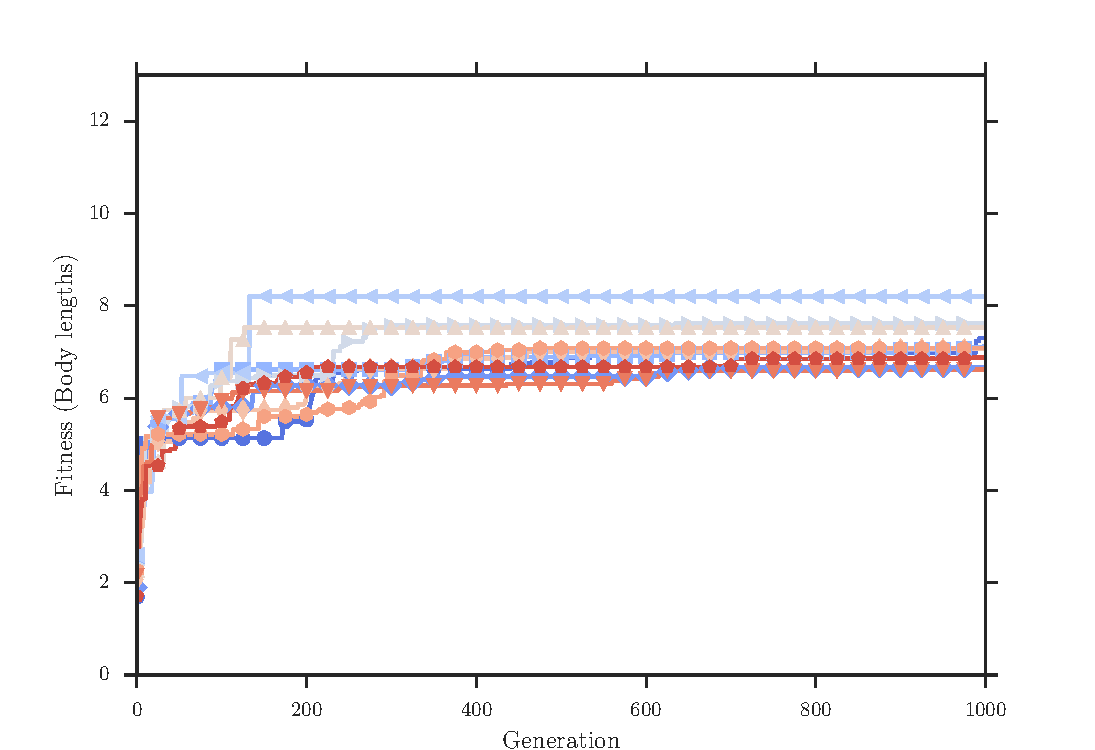
\includegraphics[width=1.0\textwidth]{../Figures/Results/indRunnAvgSize7Fitness.pdf}
\caption{Best so far fitness, $10$ individual runs for fitness based search (settings~\ref{Settings3}).}
\label{fig:indRunsAvgSize10Fitness}
\end{figure}
~
\begin{figure}[ht!]
\centering
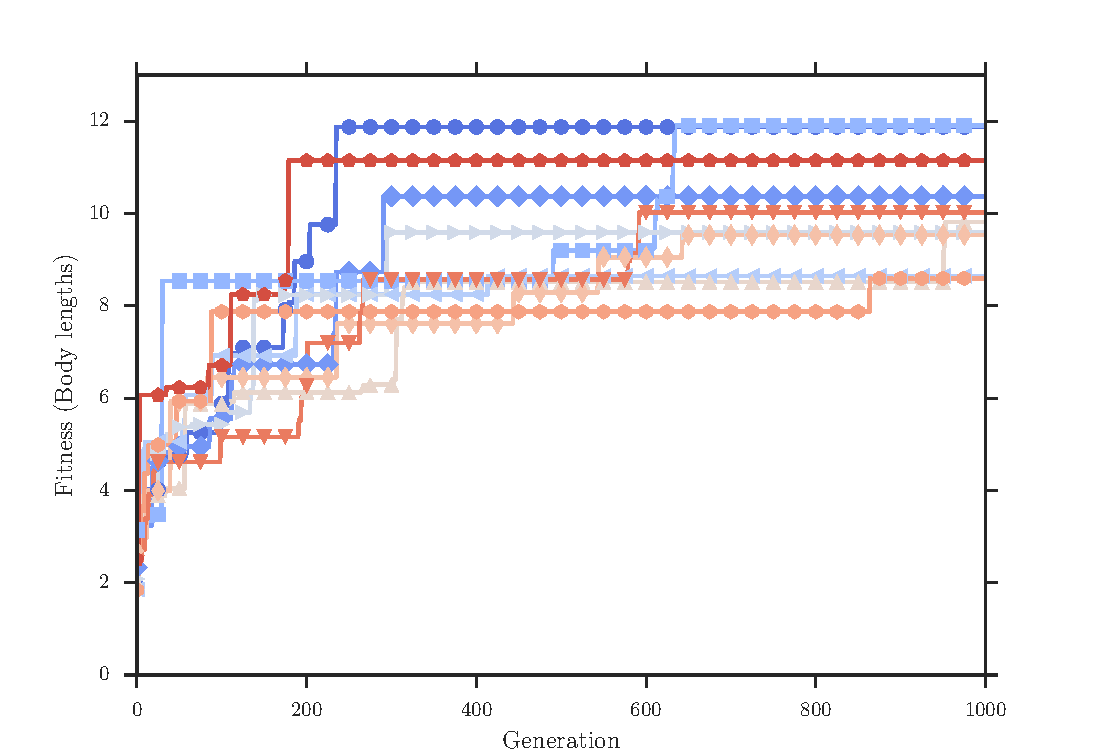
\includegraphics[width=1.0\textwidth]{../Figures/Results/indRunnAvgSize7Novelty.pdf}
\caption{Best so far fitness, $10$ individual runs for novelty search (settings~\ref{Settings3}).}
\label{fig:indRunnAvgSize10Novelty}
\end{figure}


\section{Into The Performance of Novelty Search}

Before compare novelty search to fitness based search, it is of interest to show how individually perform under the same simulation settings.

Figure~\ref{fig:indRunsAvgSize10Fitness} shows $10$ independent runs for fitness based search. Following the objective function's gradient fitness based evolution does small step towards better and more optimized individuals from generation to generation. What is more, fitness based evolution often sticks into specific morphologies which then tries to optimize leading the evolution to stop at that local maximum.

Figure~\ref{fig:indRunnAvgSize10Novelty} shows $10$ independent runs for novelty  search. In comparison with the same figure for fitness based search (fig.~\ref{fig:indRunsAvgSize10Fitness} we can see a clear difference. Evolving for novelty means that within the evolution only a novel behavior is rewarded instead of a good behavior or a behavior that leads to the optimization of the objective function. Big steps in the fitness value on all independent runs can be observed which can lead us to a conclusion that fit individuals in respect to the objective function for which novelty search has no information within the evolution process, are results of new novel behaviors. 

One more thing worth noticing, is that observing only big steps in the fitness, we can derive that there is no optimization of morphologies within novelty search. Initially, novel individuals are highly rewarded, these individuals can be very good in respect to the fitness or not, the algorithm does not consider the ``goodness'' of these individuals, and does not have any information regarding this either. On the next generation, mutations, crossovers, and copies of these novel individuals are not going to be highly variant in respect to their chromosome from their ancestors, resulting to similar behaviors, which are  not going to be remarkably rewarded in respect to their novelty value. Thus, highly novel individuals are producing less novel children, meaning that these children, even though their fitness is high and can be optimized further, will not have the chance to reproduce in the next generations and be improved eventually, as in fitness based evolution.

\begin{figure}[t!]
\centering
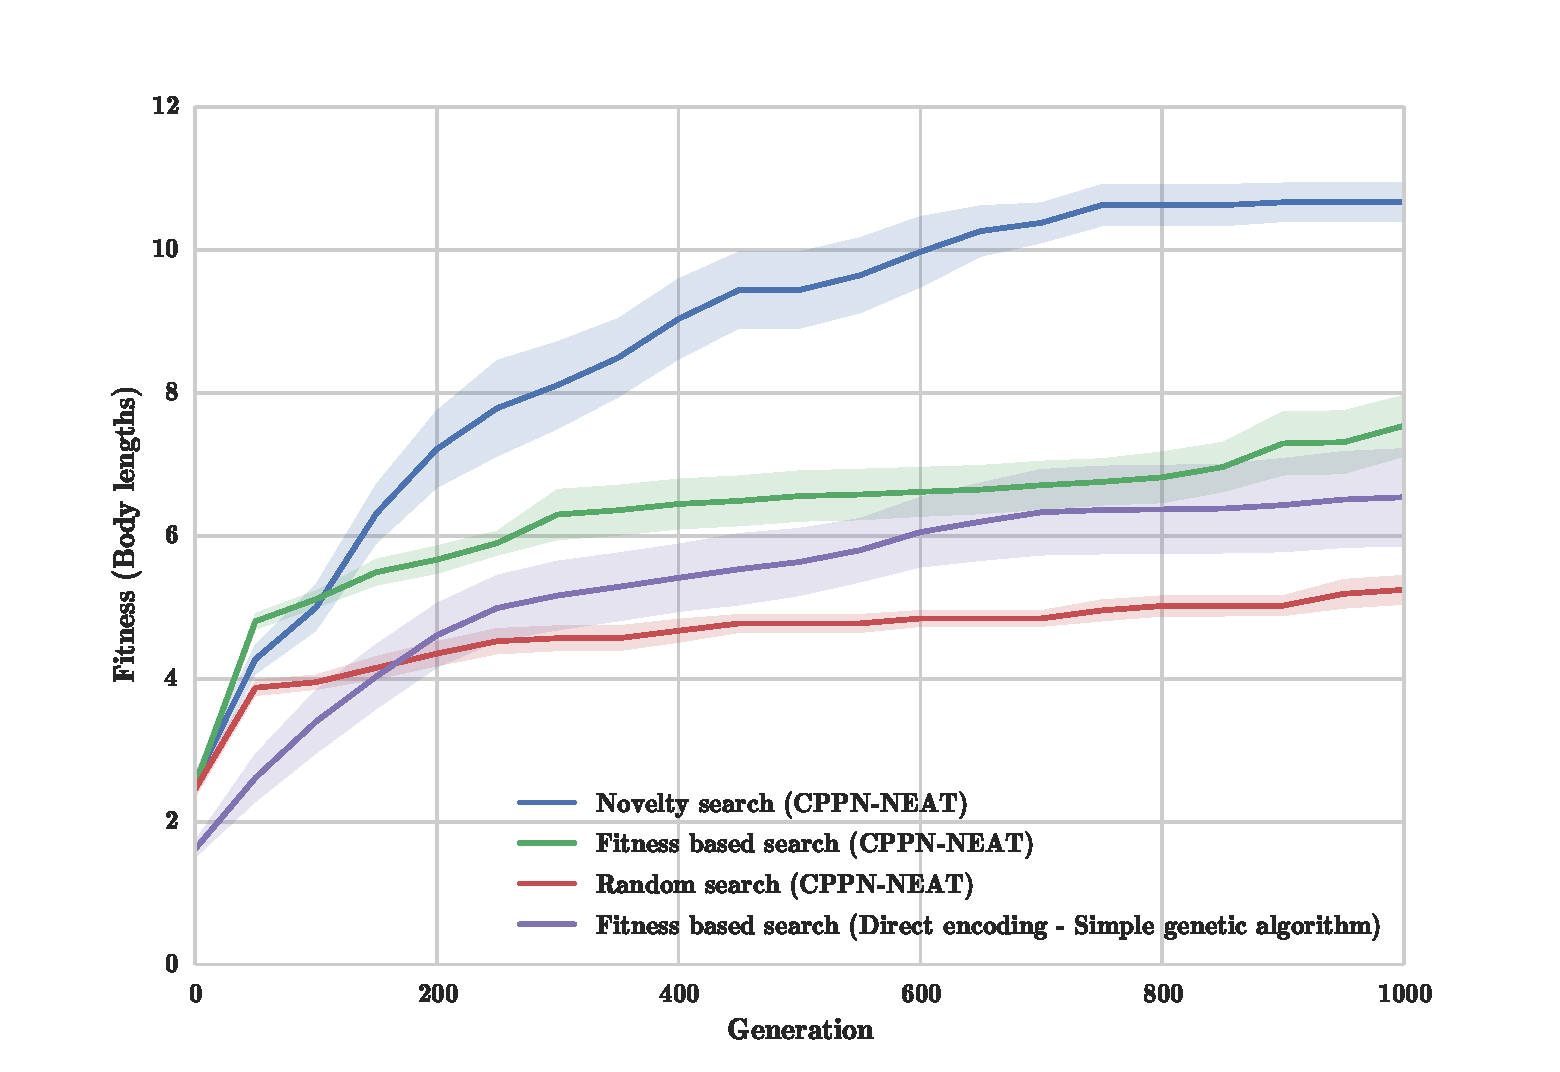
\includegraphics[width=1.0\textwidth]{../Figures/Results/FitNovRandomDirectSize5.pdf}
\caption{Comparison of simple genetic algorithm (direct encoding) against \emph{random} - \emph{fitness} - \emph{novelty} search with generative encoding. Best so far fitness averaged over $10$ runs (settings~\ref{Settings1}).}
\label{fig:FitNovRandomDirectSize5}
\end{figure}

\begin{figure}[t!]
\centering
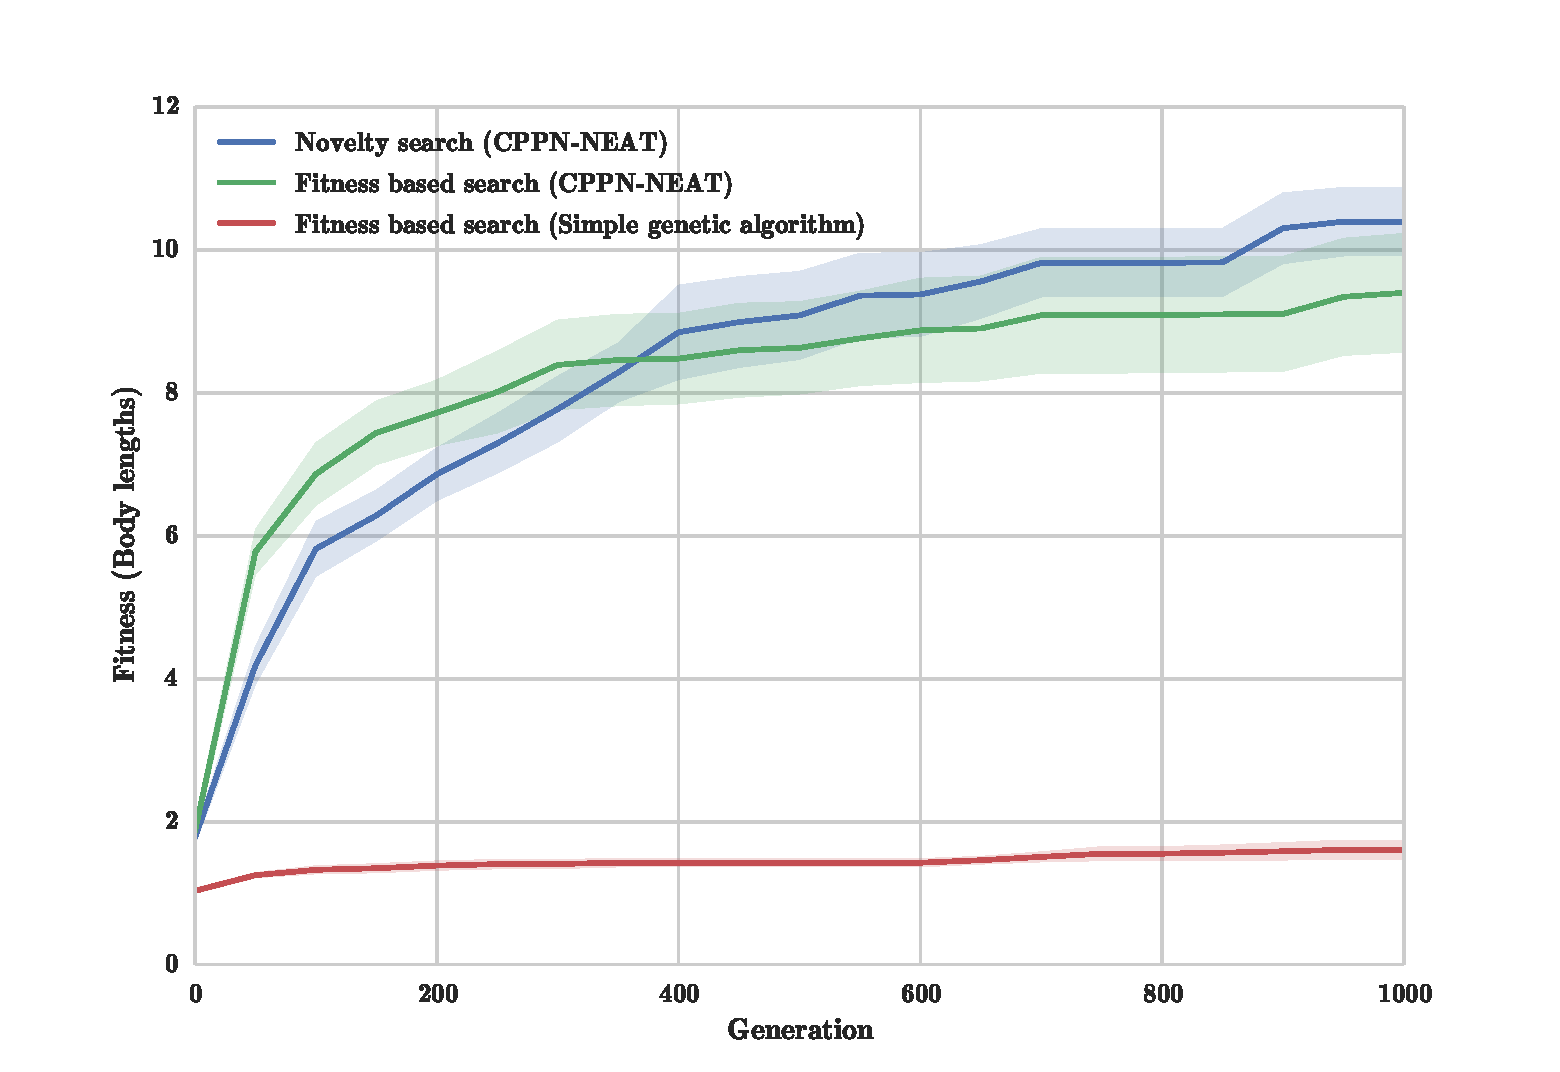
\includegraphics[width=1.0\textwidth]{../Figures/Results/FitvsNovVsDirSize10.pdf}
\caption{Comparison of simple genetic algorithm (direct encoding) against \emph{fitness} - \emph{novelty} search with generative encoding. Best so far fitness averaged over $10$ runs (settings~\ref{Settings2}).}
\label{fig:FitvsNovVsDirSize10}
\end{figure}

To extensively compare the performance achieved by novelty search method the same experiment held under two different simulation settings (for sizes $5^3$ ,$10^3$), set side by side with fitness search, random search, and finally a simple genetic algorithm. Notice, that the first three methods are referring to a generative encoding (CPPNs) evolved by Hypercube NEAT evolutionary algorithm and using selection in respect to fitness, novelty and finally random selection, while the latter uses a direct encoding scheme driven by fitness. 

Novelty search to perform the novelty metric computation, makes use of the two dimensional trajectories, which are all normalized so that their centre of mass of the trajectories coordinates meet a specific angle, as well as their starting coordinate is always located in the beginning of both axes. Fitness-based search objective function is the displacement of the soft-robot's center of mass from its initial position in body-lengths. Random evolution with Hypercube NEAT achieved using random selected individuals to breed. For direct encoding, the method used is has been explained in Chapter~\ref{Method}. 

Figure~\ref{fig:FitNovRandomDirectSize5}, presents the results for the small sized structures ($5^3$). Notice, the difference between novelty search and fitness-based method, novelty evolves structures that are superior than any other method does in these settings. At this point, it should be mentioned that in such a small structures locomotion patterns cannot be evolved due to the stability issues of the simulator, and due to the fact that lightweight structures can be bouncy, leading to ball shaped structures capable of achieving large displacement from their initial positions. That being said, we still have to deal with an optimization problem, where local optima and global ones can be found as the number of the possible solutions in this setting, using 4 materials, is $\sim 2,3 \times 10^{87}$. Using the trajectories of the soft-robots, novelty search visits optimal solutions that none of the other methods does because of local optima (fitness-based search), due to encoding limitations (direct encoding), or random search which selects random individuals to reproduce without caring about their performance, and with no backtracking (there is no guarantee that random search will visit new behaviors). The simple genetic algorithm approach which uses a direct encoding to represent the structure of the soft-robots performs better than using random selection within an indirect encoding evolution pointing out that symmetry does not provide any merits to the evolution for these sizes soft-body robots.

Moving to a larger lattice space size we expect indirect encoding to prove its advantages over the direct encoding scheme~\cite{cheney2013unshackling,stanley2007compositional}. Furthermore, novelty search now has a more difficult task as the space of possible behaviors (2d-trajectories) becomes larger as more complicated morphologies can now be produced (morphology space for $10^3$ lattice space: $9.3 \times 10^{698}$). To try to solve all these research question the same experiment held under a lattice of size $10^3$. 

Figure~\ref{fig:FitvsNovVsDirSize10}, presents the results of the same four different methods in this setting. Results reassure that novelty search achieves higher fitness on average against fitness-based search. Nevertheless, there is no tremendous difference as in the previous experiment, discovering that at their individual runs they both achieve to evolve the soft-robot structure with the highest fitness found in all experiments ($\sim 14$ Body lengths). Novelty search seems more constant in evolving individuals with high fitness in all runs, on the other hand most of individual runs of fitness search trapped in a low fitness local optimum structure, trying to optimize the specific individual genotype without trying to explore more the fitness landscape like novelty did successfully. Once again, random evolution with Hypercube NEAT is producing decent structures for soft-robots but cannot climb the hill of fitness, going in every direction, at the same time making more and more complex network topologies for CPPNs. Earlier in this thesis, in chapter~\ref{Background}, generative encoding advantages over direct explained in detail, here their superiority can evidently be observed. Direct encoding performance when a larger lattice for the simulation used, was radically decreased, mostly because structure and morphology regularity is a necessity for the soft-robots in order to perform decently in these sizes, something that direct encoding cannot capture failing to produce anything useful.






\begin{figure}[t!]
\centering
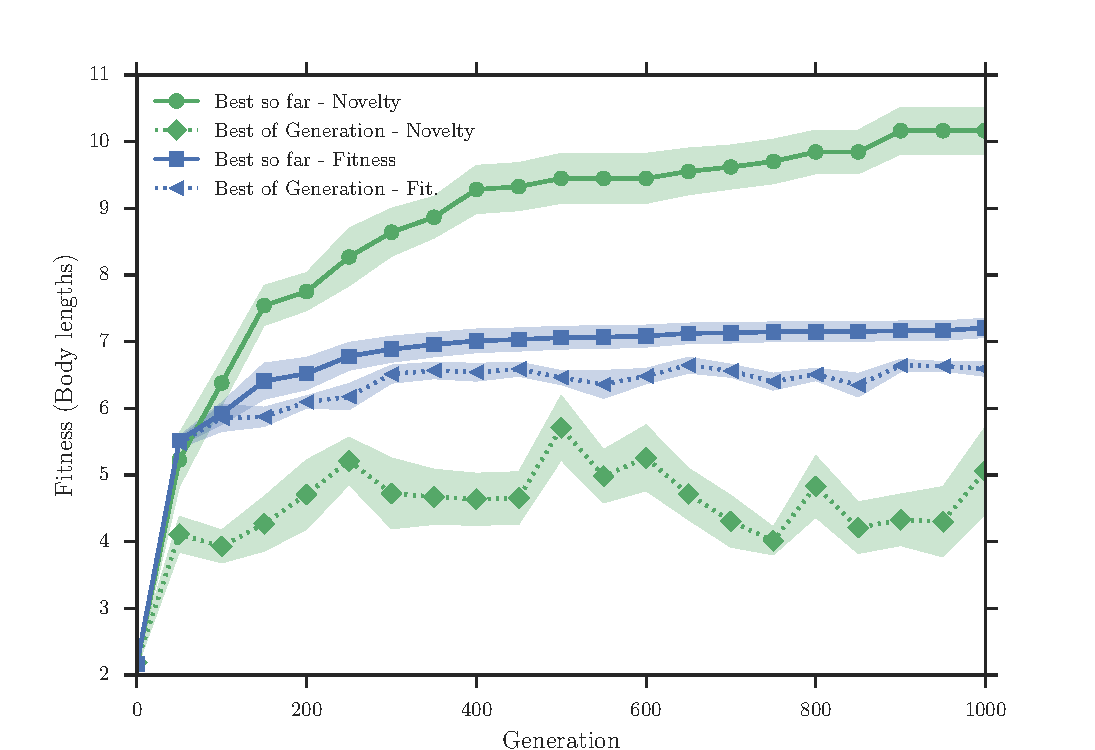
\includegraphics[width=1.0\textwidth]{../Figures/Results/AvgGenerChampNoveltyFitnessSize7.pdf}
\caption{Fitness of the generation's champion (best individual) for \emph{fitness} - \emph{novelty} search averaged over $10$ runs (settings~\ref{Settings3}).}
\label{fig:AvgGenerChampNoveltyFitnessSize7}
\end{figure}

Another aspect of the evolution should be inspected is how the population of each generation is affected in respect to the best individual per generation, especially thinking about the these generation champions is the ones that result in the increased of novelty search when compared with fitness based search. In figure~\ref{fig:AvgGenerChampNoveltyFitnessSize7}, the champions' fitness (Best fitness found within each generation) of each generation is plotted averaged over $10$ runs. Recall, that novelty search does not have any information about fitness of individuals. In fitness based search there is a clear trend that champions of each generation are getting better through the evolution resulting to an approximately monotonically increasing function. On the other hand, generations' champions in novelty search apart from the early improvement which is mainly caused by the generative encoding, follow a random pattern. What it is interesting here to see is that even though that the solutions novelty search gives, in this settings (lattice size: $7^3$), are clearly better than the ones evolved by fitness based search, on average the champions during novelty search evolution are worse. Hence, individuals that resulting in the increased performance of novelty search clearly lie on the tail of the fitness distribution on each generation.


\begin{figure}[t!]
\centering
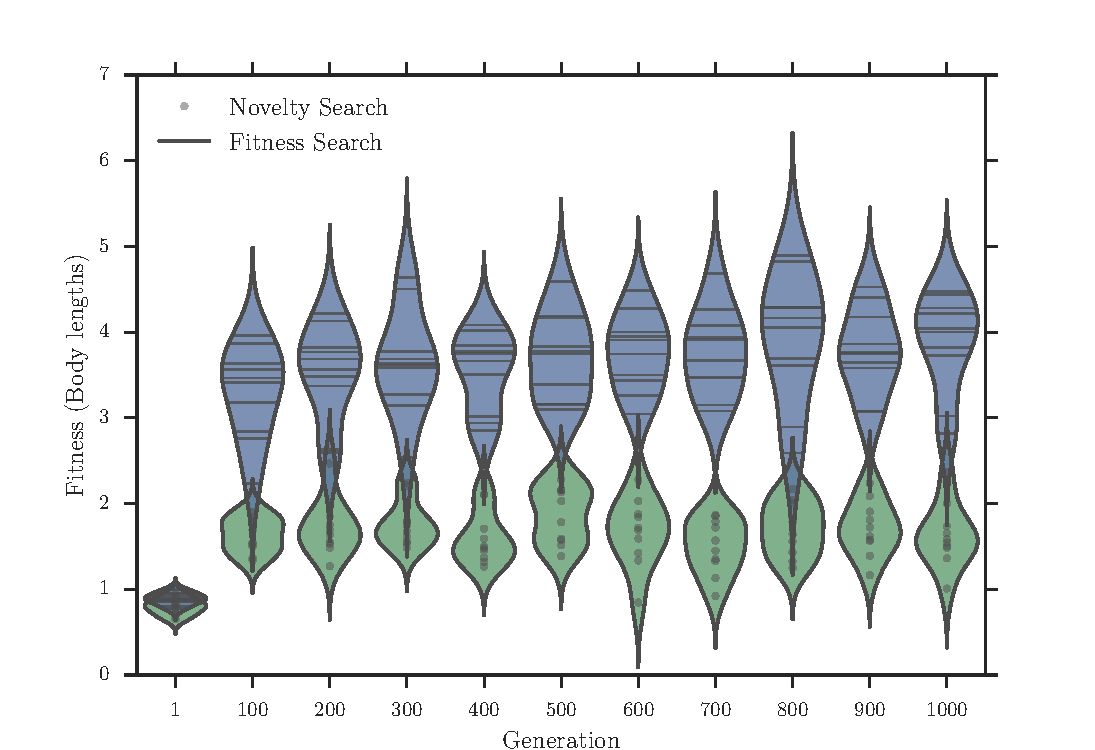
\includegraphics[width=1.0\textwidth]{../Figures/Results/ViolinPlotsAvgGenFitSize7.pdf}
\caption{Distributions of average population fitness per generation over 10 runs for \emph{fitness}(Blue) - \emph{novelty} (Green) search with generative encoding (settings~\ref{Settings3}).}
\label{fig:ViolinPlotsAvgGenFitSize7}
\end{figure}

In the same fashion, the average population fitness seems also affected by the different optimization methods. Figure~\ref{fig:ViolinPlotsAvgGenFitSize7} illustrates the distribution of population's average fitness over $10$ independent runs for \emph{novelty}-\emph{fitness} based search every $100$ generations. The resulted distributions which are shown in violin-like shapes clearly show that the average generation's fitness remains stable through the whole evolution ($1000$ generations) for both methods. What is more, the generation's average fitness is significantly lower for \emph{novelty} search, meaning that when the evolution is being carried towards novel behaviors there is no such guarantee that assumes novel new founds in the behavioral space will also be \emph{fit}. 

What we see in the last two figures, evidently shows that even though novelty search achieves in finding more ``fit'' solutions than fitness based search in the specific problem domain, the average fitness of both generation champions and population remain lower than in fitness based search.

\begin{figure}[t!]
\centering
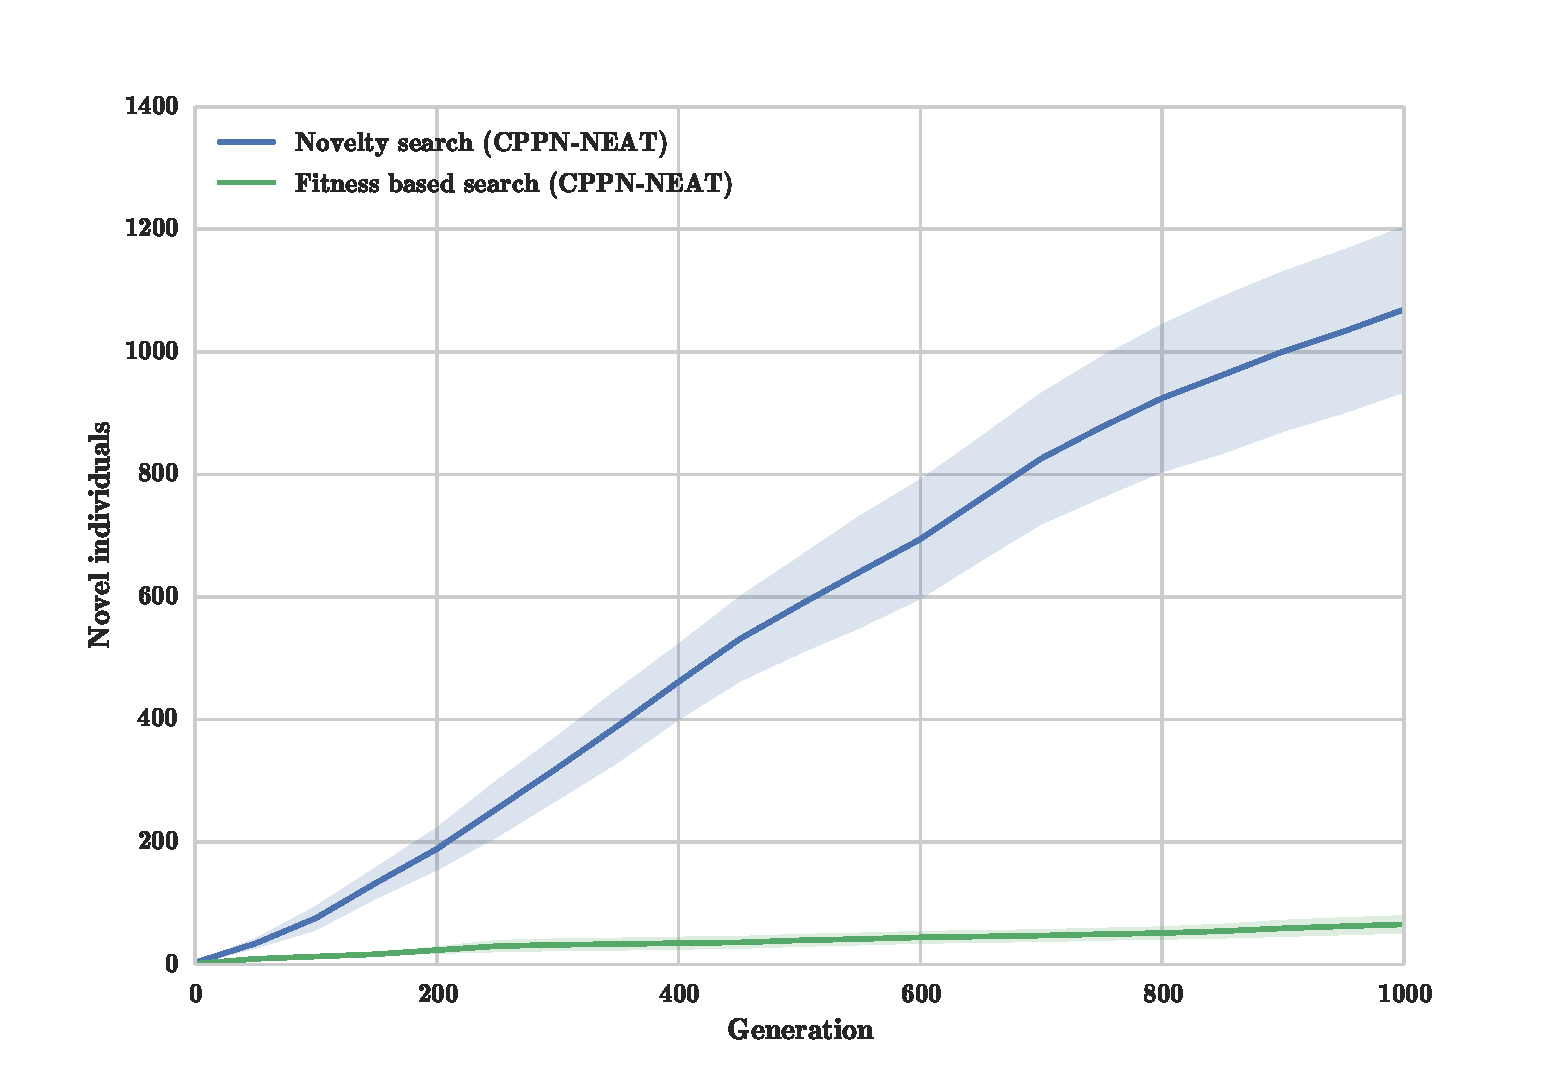
\includegraphics[width=1.0\textwidth]{../Figures/Results/novelIndividualsFitNovComp.pdf}
\caption{Number of novel behaviors found up to generation number, averaged over 10 runs. The novelty measure is computed as the average distance from the $10$-nearest behaviors for \emph{fitness} - \emph{novelty} search with generative encoding (settings~\ref{Settings3}).}
\label{fig:novelIndividualsFitNovComp}
\end{figure}

Until this point, the performance of both fitness and novelty search methods have been compared in the same objective metric such as the displacement of the produced soft body robots. The former method method tries to optimize genomes in respect to the specific objective function, while the latter moves its interest into creating diversity of the population in the behavioral space. As shown before, the novelty search achieves to create novel individuals which are not only novel in respect to how different behaviors they have from the rest of the population they exist into, but also they achieve higher average fitness than those they are optimized towards that objective. Inverting the objective function now such as our goal is to generate a wide variety of behaviors, in this case, two dimensional trajectories, we expect that a much larger set of novel behaviors will be created by novelty search. Figure~\ref{fig:novelIndividualsFitNovComp}, presents the number of unique behaviors the two evolutionary methods found, averaged over $10$ runs. The resulted graph shows that comparing these two methods is pointless as \emph{novelty} search can force the evolution towards spaces in the behavioral space that have not visited, finding more novel individuals, which does not happen in the fitness search. Surprisingly, \emph{novelty} achieves better performance than \emph{fitness} search in both objectives set so far, creating fit, and at the same time diverse solutions.

\begin{figure}[t!]
\centering
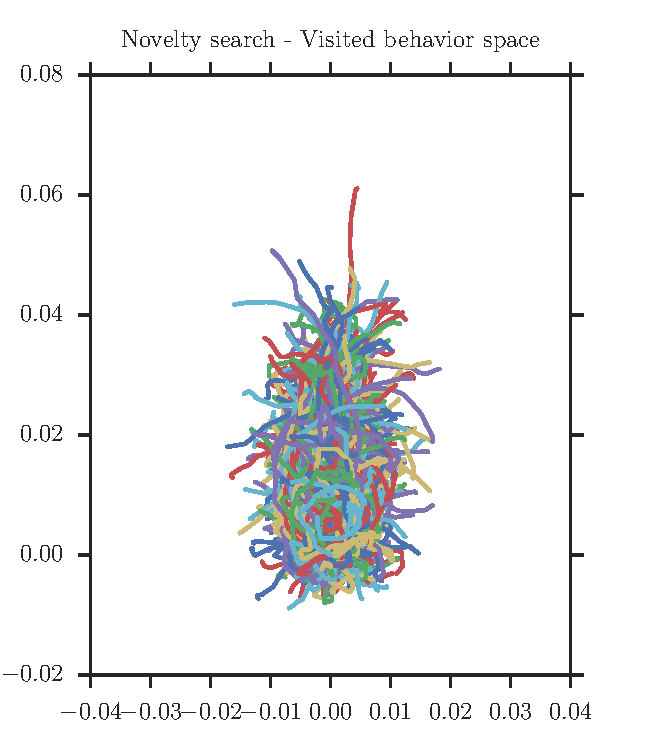
\includegraphics[width=0.49\textwidth]{../Figures/Behaviors/behaviorsNovelty.pdf}\	
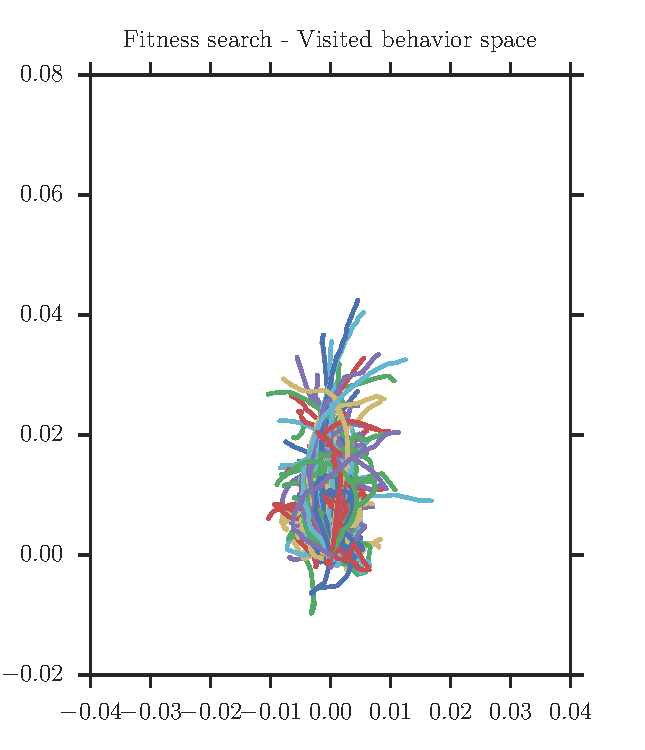
\includegraphics[width=0.49\textwidth]{../Figures/Behaviors/behaviorsFitness.pdf}
\caption{Novelty search creates a vast amount of behaviors achieving in this way to find fit individuals, and avoid local optima of the solution space. (settings~\ref{Settings3})}
\label{fig:behaviorSpaceDiversity}
\end{figure}

To visualize the difference in the behavior space of the two methods, figure~\ref{fig:behaviorSpaceDiversity}, illustrates all the stored found novel behaviors (two dimensional trajectories) found in one evolution run of novelty and fitness search using the same novel measure to determine the novelty of a behavior.




\subsection{How Behavior Selection Affects \emph{Novelty}-Search}

A good behavior metric should include information about the objective function. In case of locomotion gait of soft robots a trajectory can be highly informative as far as the displacement of the robot's body, as well as the gait, is concerned. Two robot bodies which travelled the same distance into an equal time horizon, should have the same fitness if displacement is only measured, nevertheless, the locomotion strategy, is something that can only affect the actual behavior metric and not the objective function. Forcing the evolution to seek for the novel in the behavior space results in producing $>10 \times$ more novel behaviors than \emph{fitness} search (depending on the threshold and the behavior metric), which  indirectly implies that high fitness individuals will be found as the behavior space is heavily searched. How the behavior metric affects the performance of the evolution is discussed in detail in the next section.

\begin{figure}
\centering
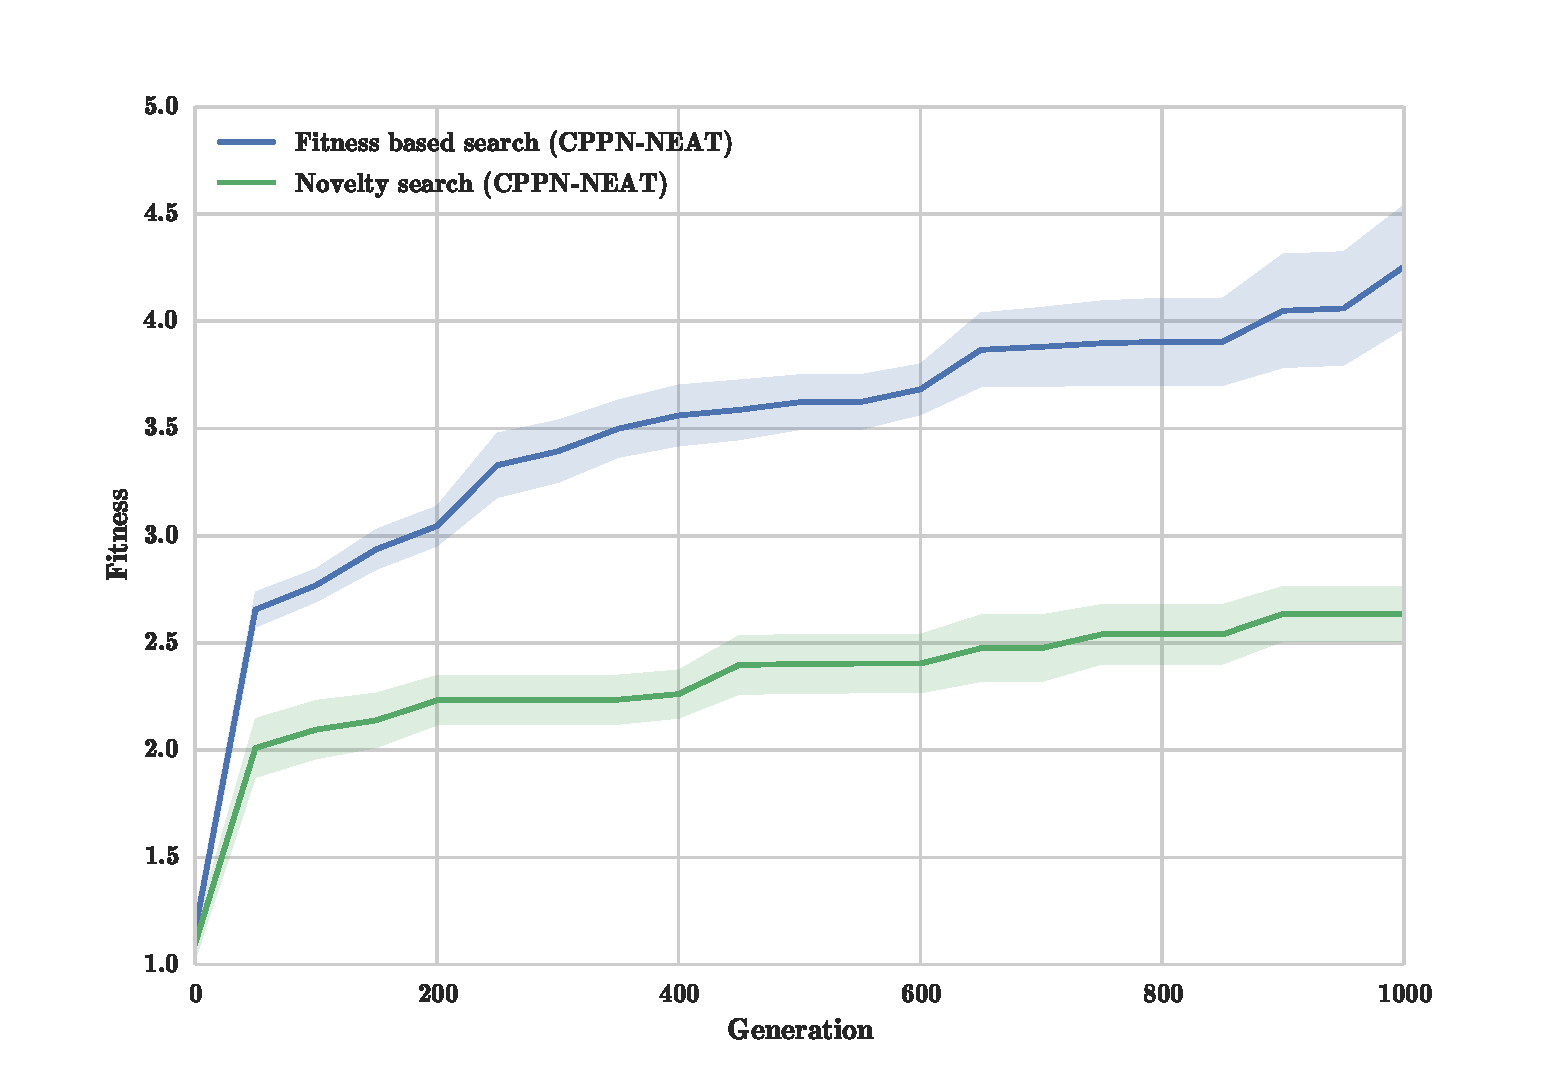
\includegraphics[width=1.0\textwidth]{../Figures/Results/FitNovSize5Pen2.pdf}
\caption[]{Best so far fitness averaged over $10$ runs, penalizing actuated materials\footnotemark for \emph{fitness} - \emph{novelty} search with generative encoding (settings~\ref{Settings1}).}
\label{fig:FitNovSize5Pen2}
\end{figure}

\footnotetext{Actuated materials penalize fitness: \[f = (1 - (n_{actuated} / n_{total})^{1.5}) \times disp \], where $n_{actuated}$, is the number of actuated voxels, $n_{total}$ total number of voxels and $disp$ the displacement of the softbot's center of mass.}


The importance of selecting a good behavior metric is important in order for novelty search to explore the behavior space to a great extent. For example, searching for fast robots while you exploring the behavior space of their trajectories is a wise decision considering that all information needed to determine the fitness (speed) is incorporated inside the behavior (trajectories) assuming static sampling rate of the trajectories. In this experiment to investigate what is the result of the novelty-search evolution when no information about fitness is provided by the behavior, a objective function was selected that the currently used behavior metric doe not include information about. The two dimensional projection of the trajectories in $x,y$-axis are again selected, while instead of evaluating the fitness in displacement, this displacement is penalized by the number of actuated voxels are inside the structure of the soft robot. Figure~\ref{fig:FitNovSize5Pen2}, illustrates the best so far fitness for both novelty and fitness search averaged on $10$ independent runs. Comparing the results with figure~\ref{fig:FitNovRandomDirectSize5}, one can notice how novelty search performs poorly in this setting. Considering that the same method outperforms traditional fitness-search evolution when the whole information of the fitness function is contained in the behavior. Trying to find novel trajectories in the first case proved successful in respect to the final displacement of the individuals produced. On the other hand trying to maximize the distance and in the same time use as few actuated voxels as possible, proved crucial for the final outcome of the search for novelty. If the number of actuated voxels had been included in some way into the behavior metric, novelty-search would have been more exploratory towards this direction as well.


\begin{figure}[t!]
\centering
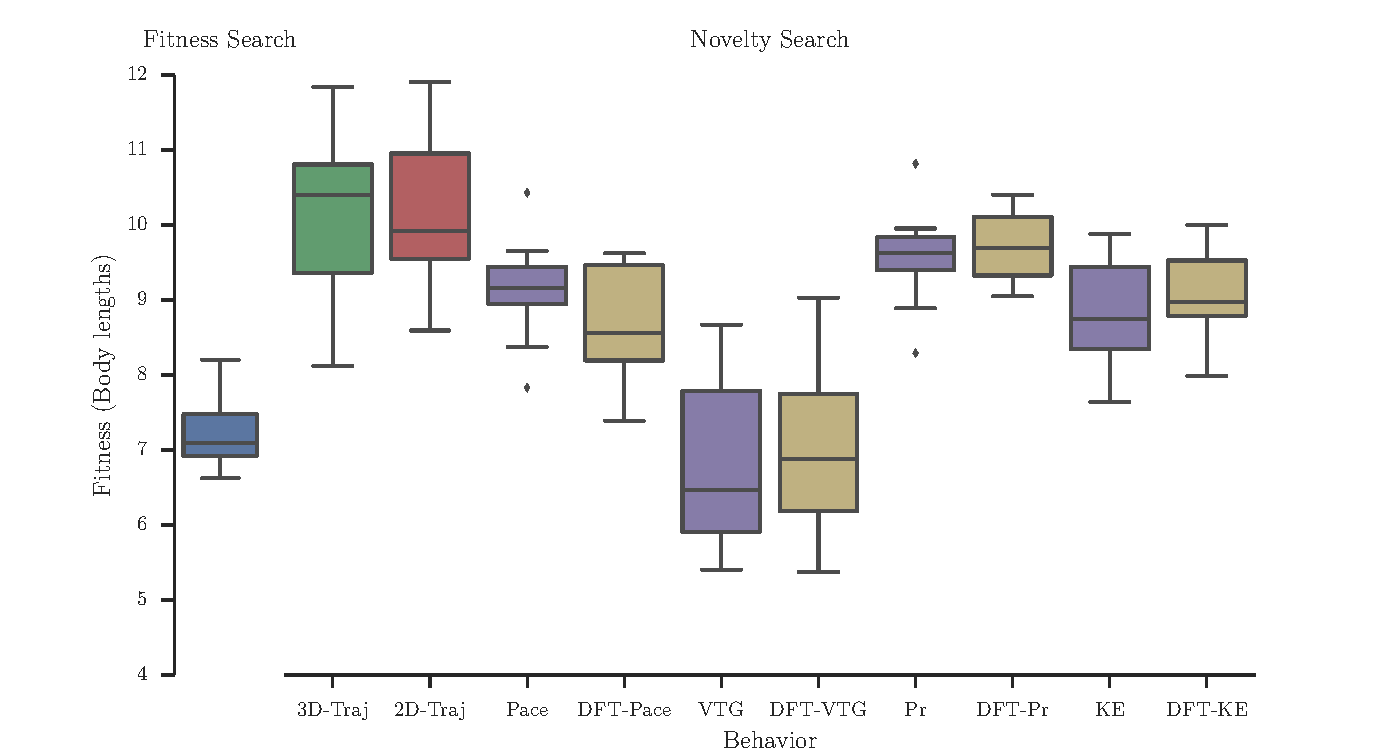
\includegraphics[width=1.0\textwidth]{../Figures/Results/BehaviorsPerformance.pdf}
\caption{Comparison of the evolution's best fitness result from $10$-runs under different behavioral metrics for \emph{novelty} search (right). \emph{Fitness} search is also evaluated under the same settings (left - \textcolor{MidnightBlue}{blue} box). (settings~\ref{Settings3}).}
\label{fig:BehaviorsPerformance}
\end{figure}


Choosing the appropriate metric to describe a phenotype into the behavior space is crucial in the performance of novelty search. Figure~\ref{fig:BehaviorsPerformance} illustrates the experimental results under different behavior metrics, alongside the performance of pure \emph{fitness} based optimization. A set of $10$ different behavior types was used including the three dimensional trajectories of the soft robots (3D-Traj), the two dimensional projection on $x,y$-axes of the previous behavior (2D-Traj), the pace sampled every $0.001$ sec. (Pace), the discrete Fourier transformation of the same signal which was sampled every $0.00001$ sec. (DFT-Pace), the voxels touching the ground on each time-step (VTG, DFT-VTG), the maximum pressure per time-step (Pr, DFT-Pr), and the kinetic energy of the whole structure (KE, DFT-KE). What is shown here, is the fitness in body lengths of the champion individual during the whole evolution from $10$-independent runs of the experiment. Both trajectory behavior types achieve the best performance as far as fitness is concerned, with a small difference in favor of the three dimensional one. Pressure is coming third achieving high performance close to the previous two trajectory behavior types, pace and kinetic energy of the structure are next in the performance ladder, and last one is the behavior signal that count how many voxels touch the ground on each sampling time-step. The results of using $10$ different behavior types can be clustered into three performance categories. The first one which includes the two types of trajectories and achieves the best performance of all, the second one which includes raw values and the discrete Fourier transformation of pace, pressure and kinetic energy, the last and worst one with the number of voxels touching the ground. 

\begin{figure}[t!]
\centering
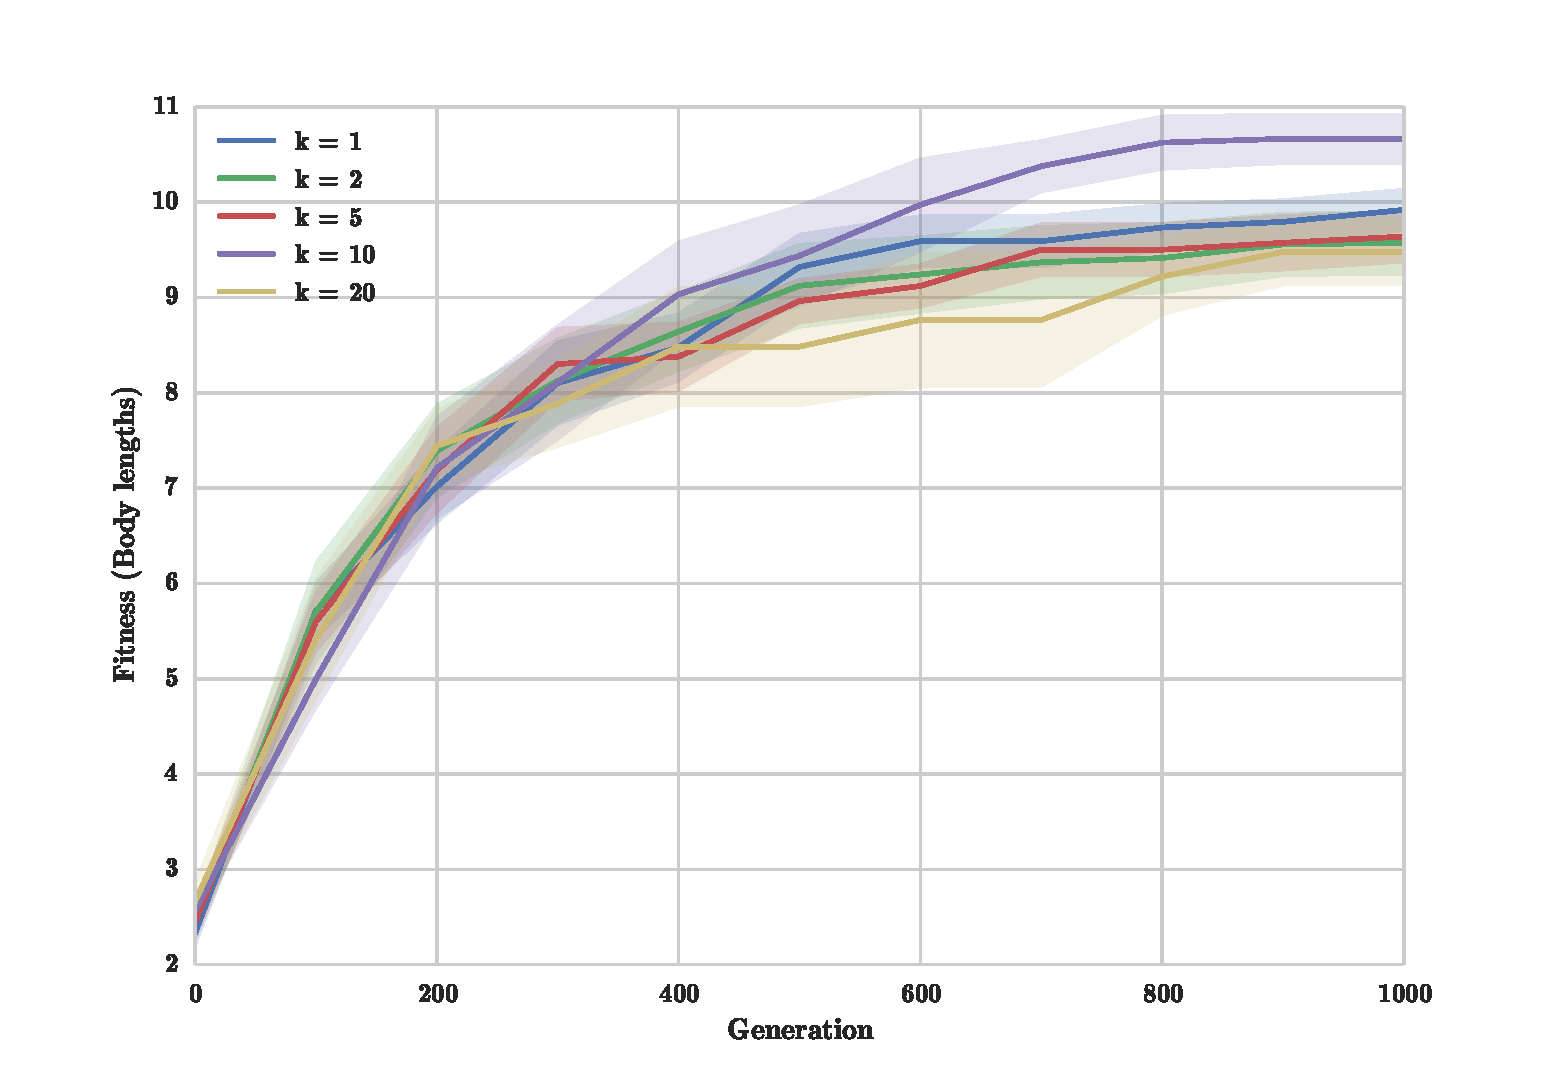
\includegraphics[width=1.0\textwidth]{../Figures/Results/KnnExperimentSize5.pdf}
\caption{Best so far fitness averaged over $10$ runs, for different $k$ to sparsity computation of the behavior (settings~\ref{Settings1}).}
\label{fig:KnnExperimentSize5}
\end{figure}

The performance of novelty search when trajectory of the soft bodies is used as a behavior metric is superior over all other behavior metrics. Trajectories are a very good selection for this kind of problem, since they can indirectly not only encode the objective function which is the displacement, but also the locomotion strategy and that is the reason why they explore better the landscape of behaviors resulting in such high difference in fitness against the fitness search. 

The rest of the behavior metrics apart from VTG and VTG-DFT, are close, as far as the final performance of the evolution is concerned. On reason that they fail to meet the trajectories performance is the fact that even though they keep track of features that can actually measure the performance of the robot, speed, they cannot encode the direction of the soft-body during the simulation. Which is crucial if we think that soft-robots having a circle trajectory, even though they can produce fast locomotion that displacement from their initial positions will remain low.

Counting the number of voxels in a structure that touch the ground in every timestep of the simulation, does not have any implication about how fast the robot is moving. A fast moving robot that is hopping can have the same behavior signature with a hopping robot that stays in the same position after each jump, yet, using the trajectories these two soft-robots will have a huge difference in their behaviors.

Within the same figure and on the left side of it (\textcolor{MidnightBlue}{blue} box), \emph{fitness}-search is also evaluated under the same experimental settings. The performance of this objective optimization method is only comparable with the worst \emph{novelty}-search scenario when the VTG behavior is selected for novelty to be measured.

\begin{figure}[t!]
\centering
\begin{subfigure}[b]{1.0\textwidth}
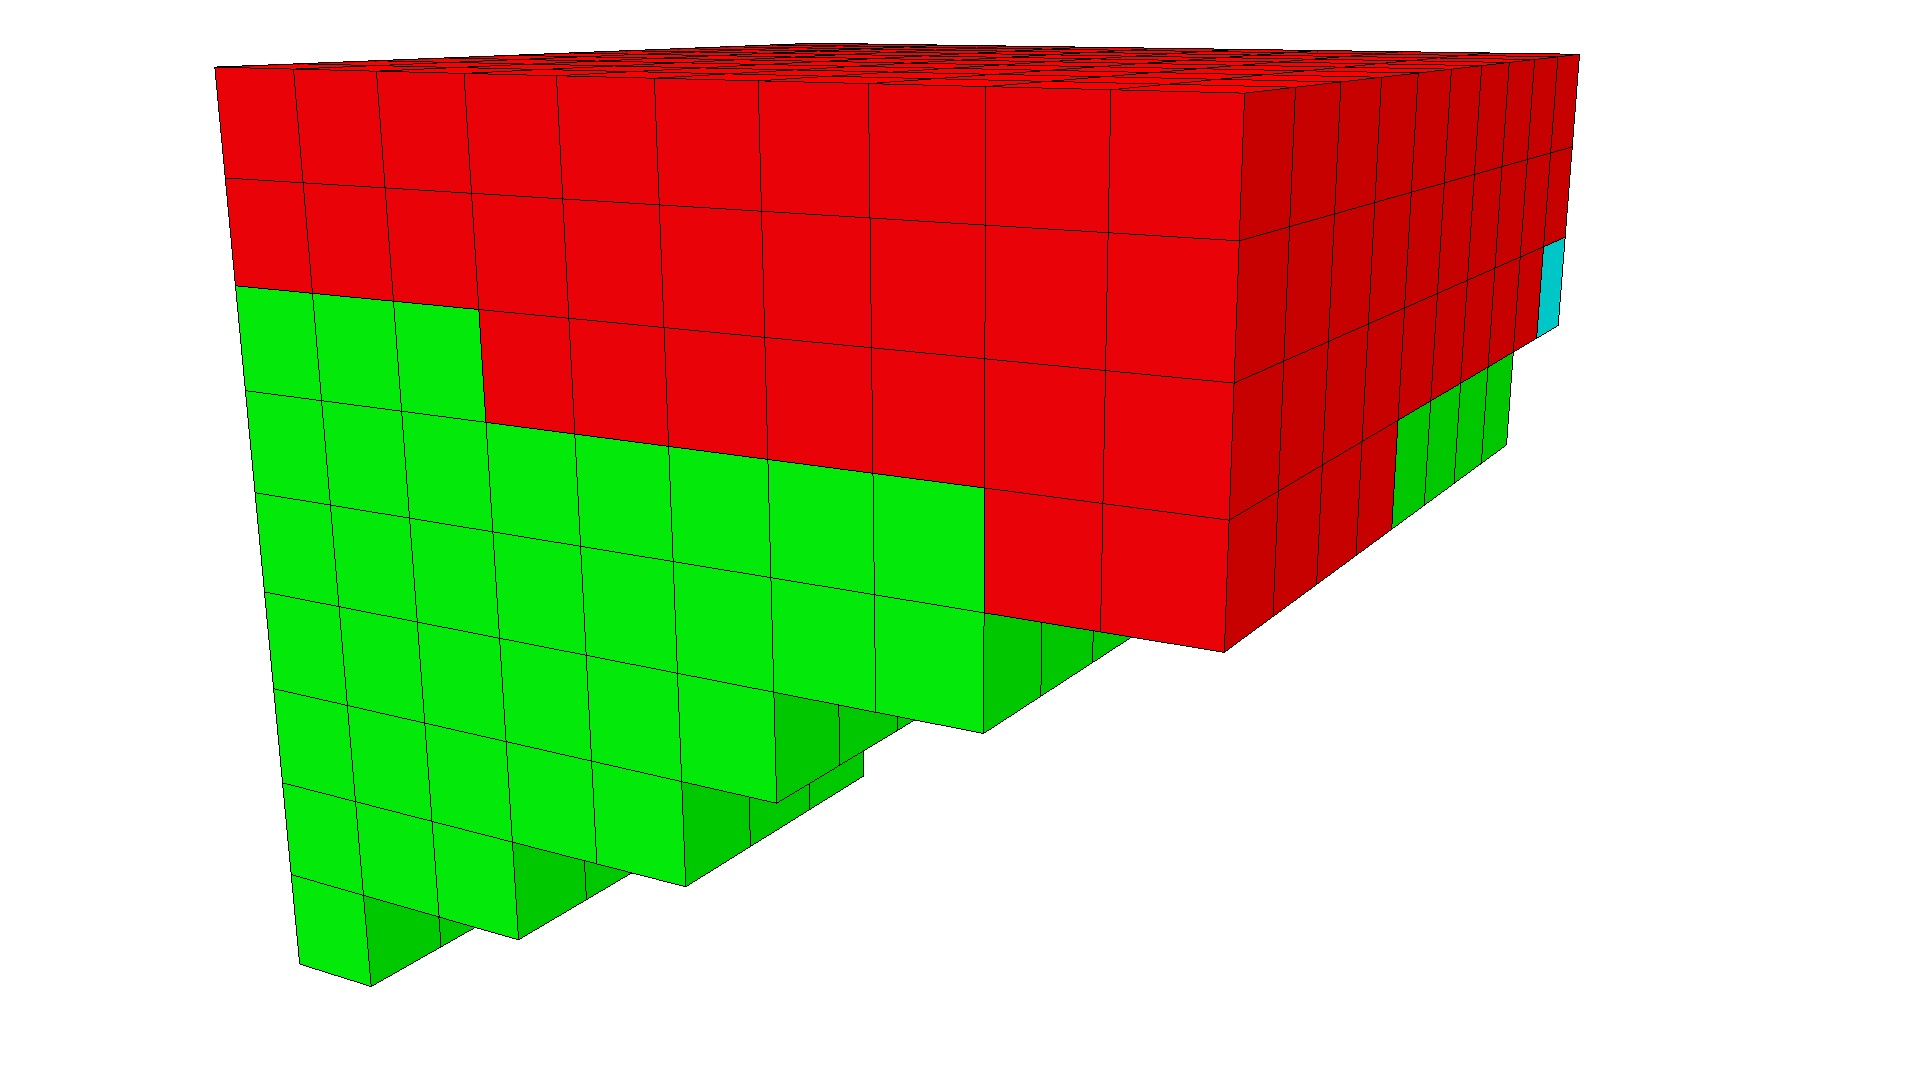
\includegraphics[width=0.19\textwidth]{../Figures/Robots/f_4_g_100.jpg}
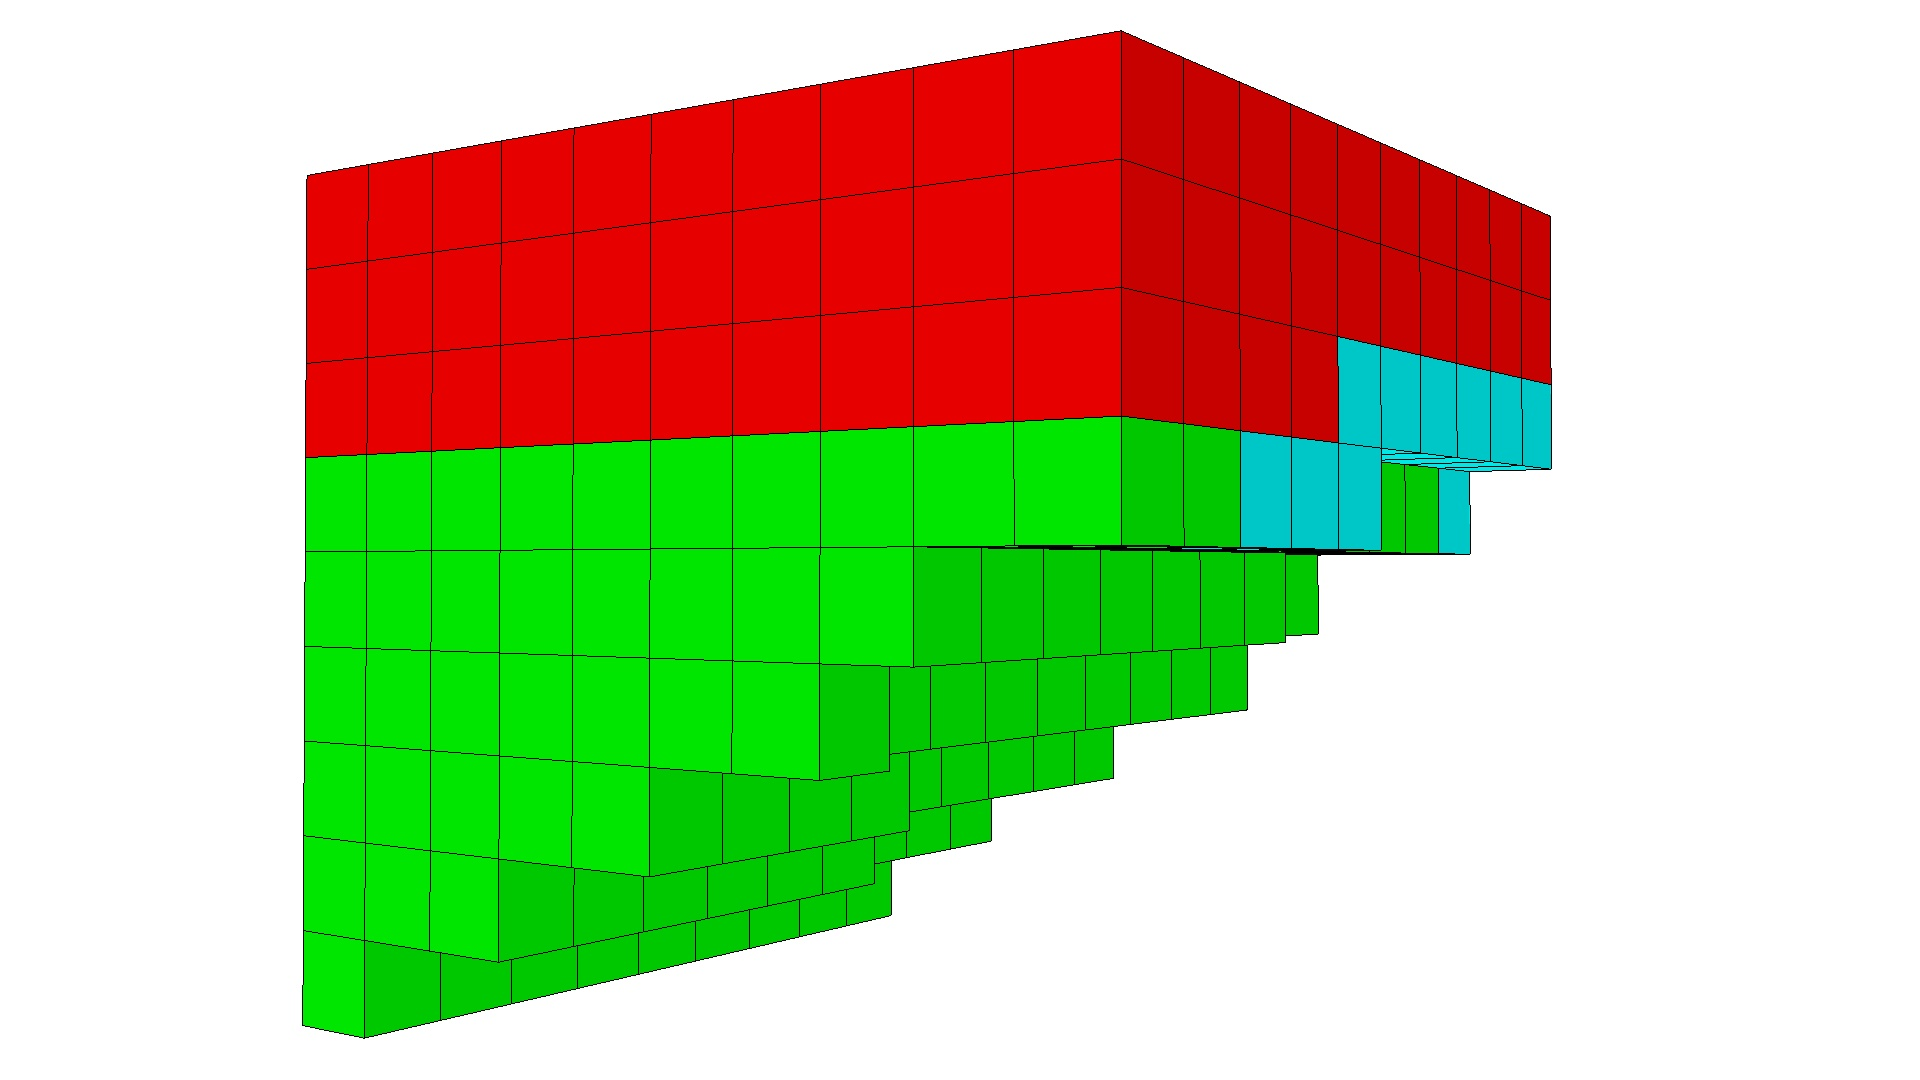
\includegraphics[width=0.19\textwidth]{../Figures/Robots/f_4_g_200.jpg}
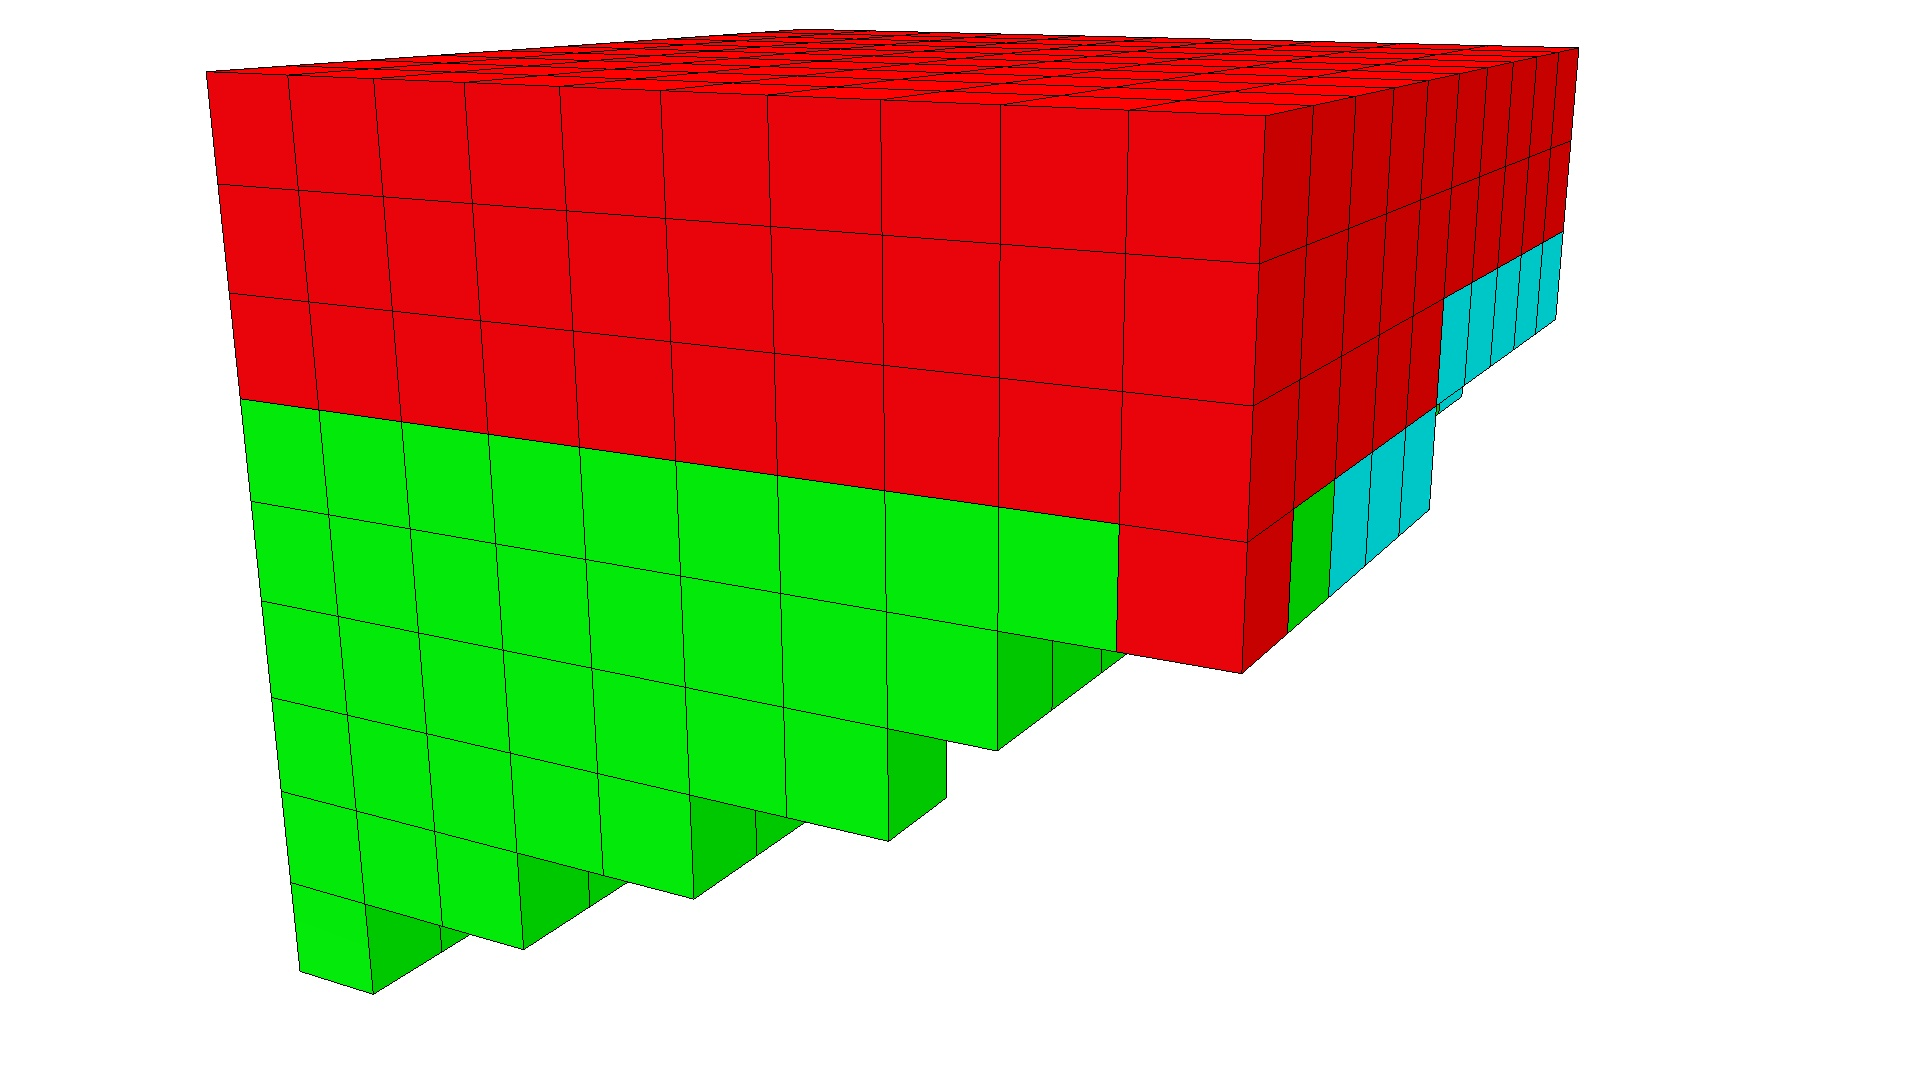
\includegraphics[width=0.19\textwidth]{../Figures/Robots/f_4_g_300.jpg}
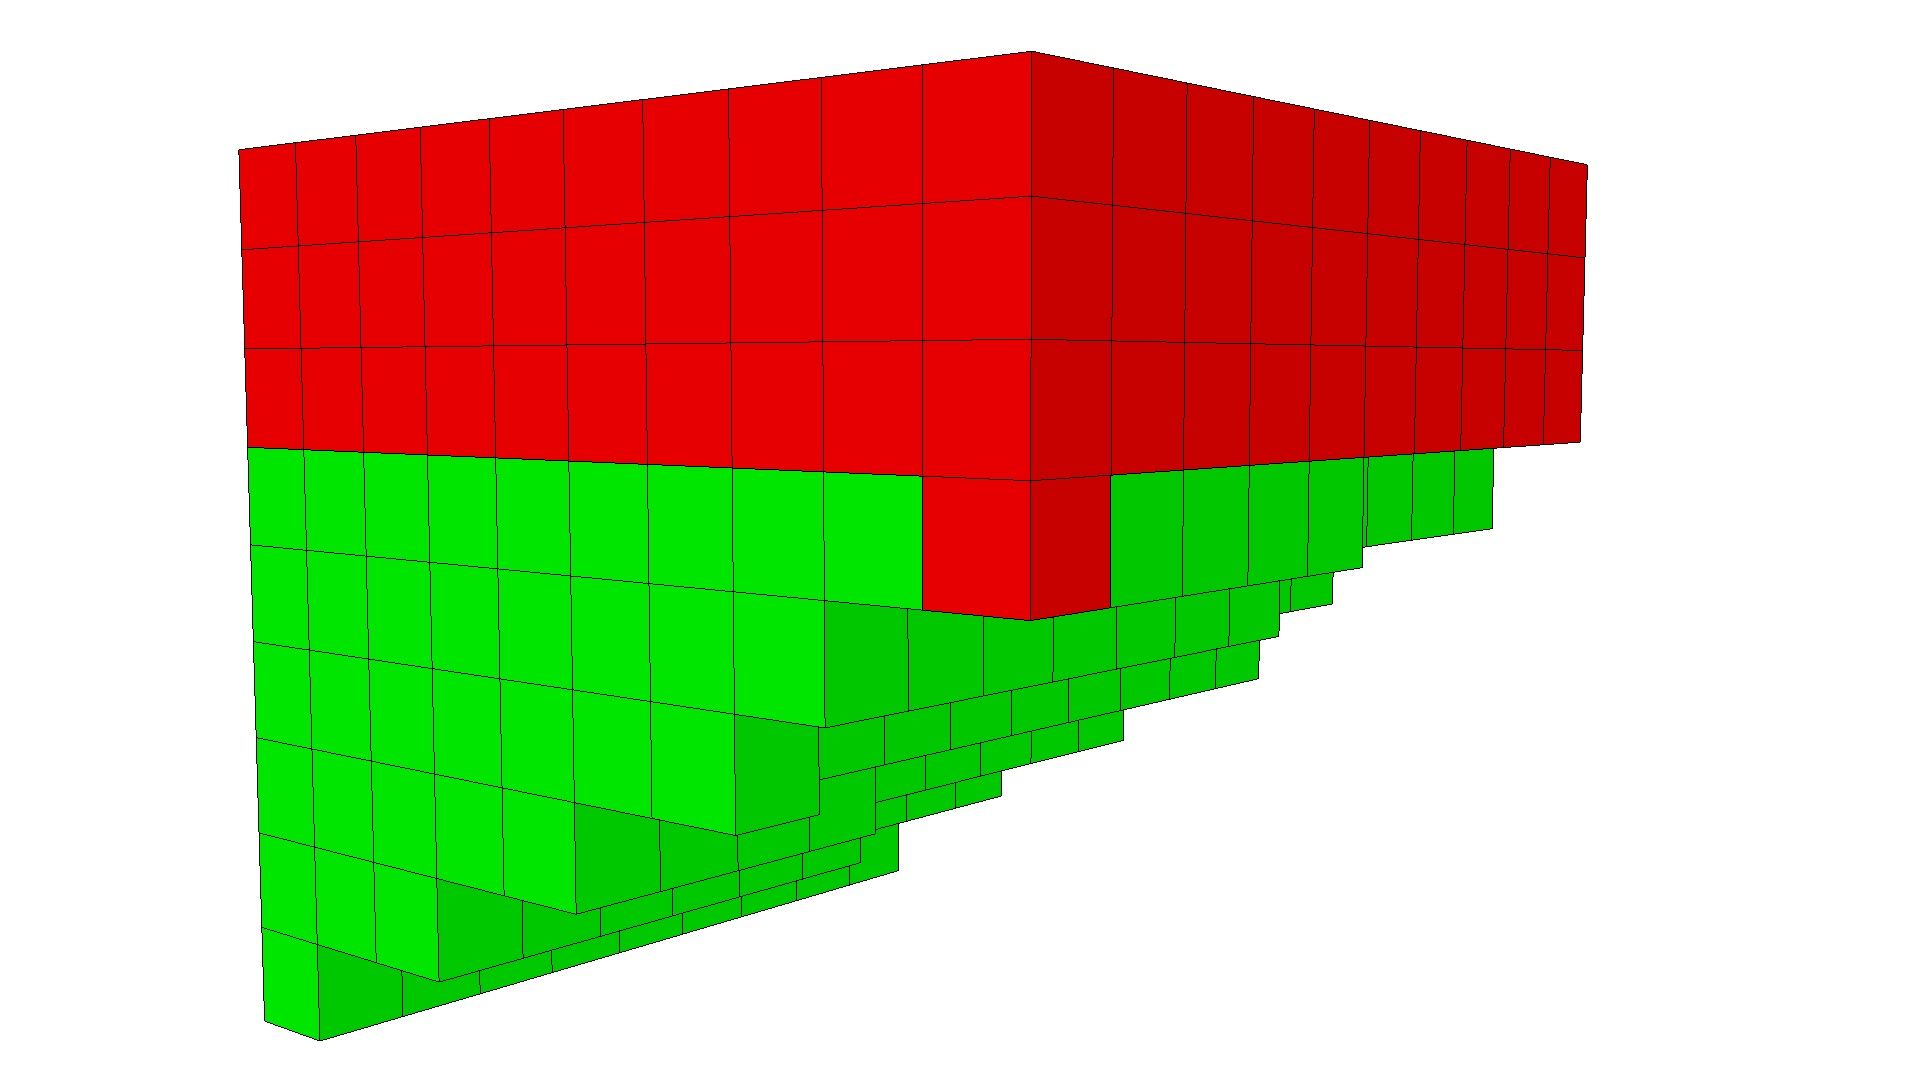
\includegraphics[width=0.19\textwidth]{../Figures/Robots/f_4_g_400.jpg}
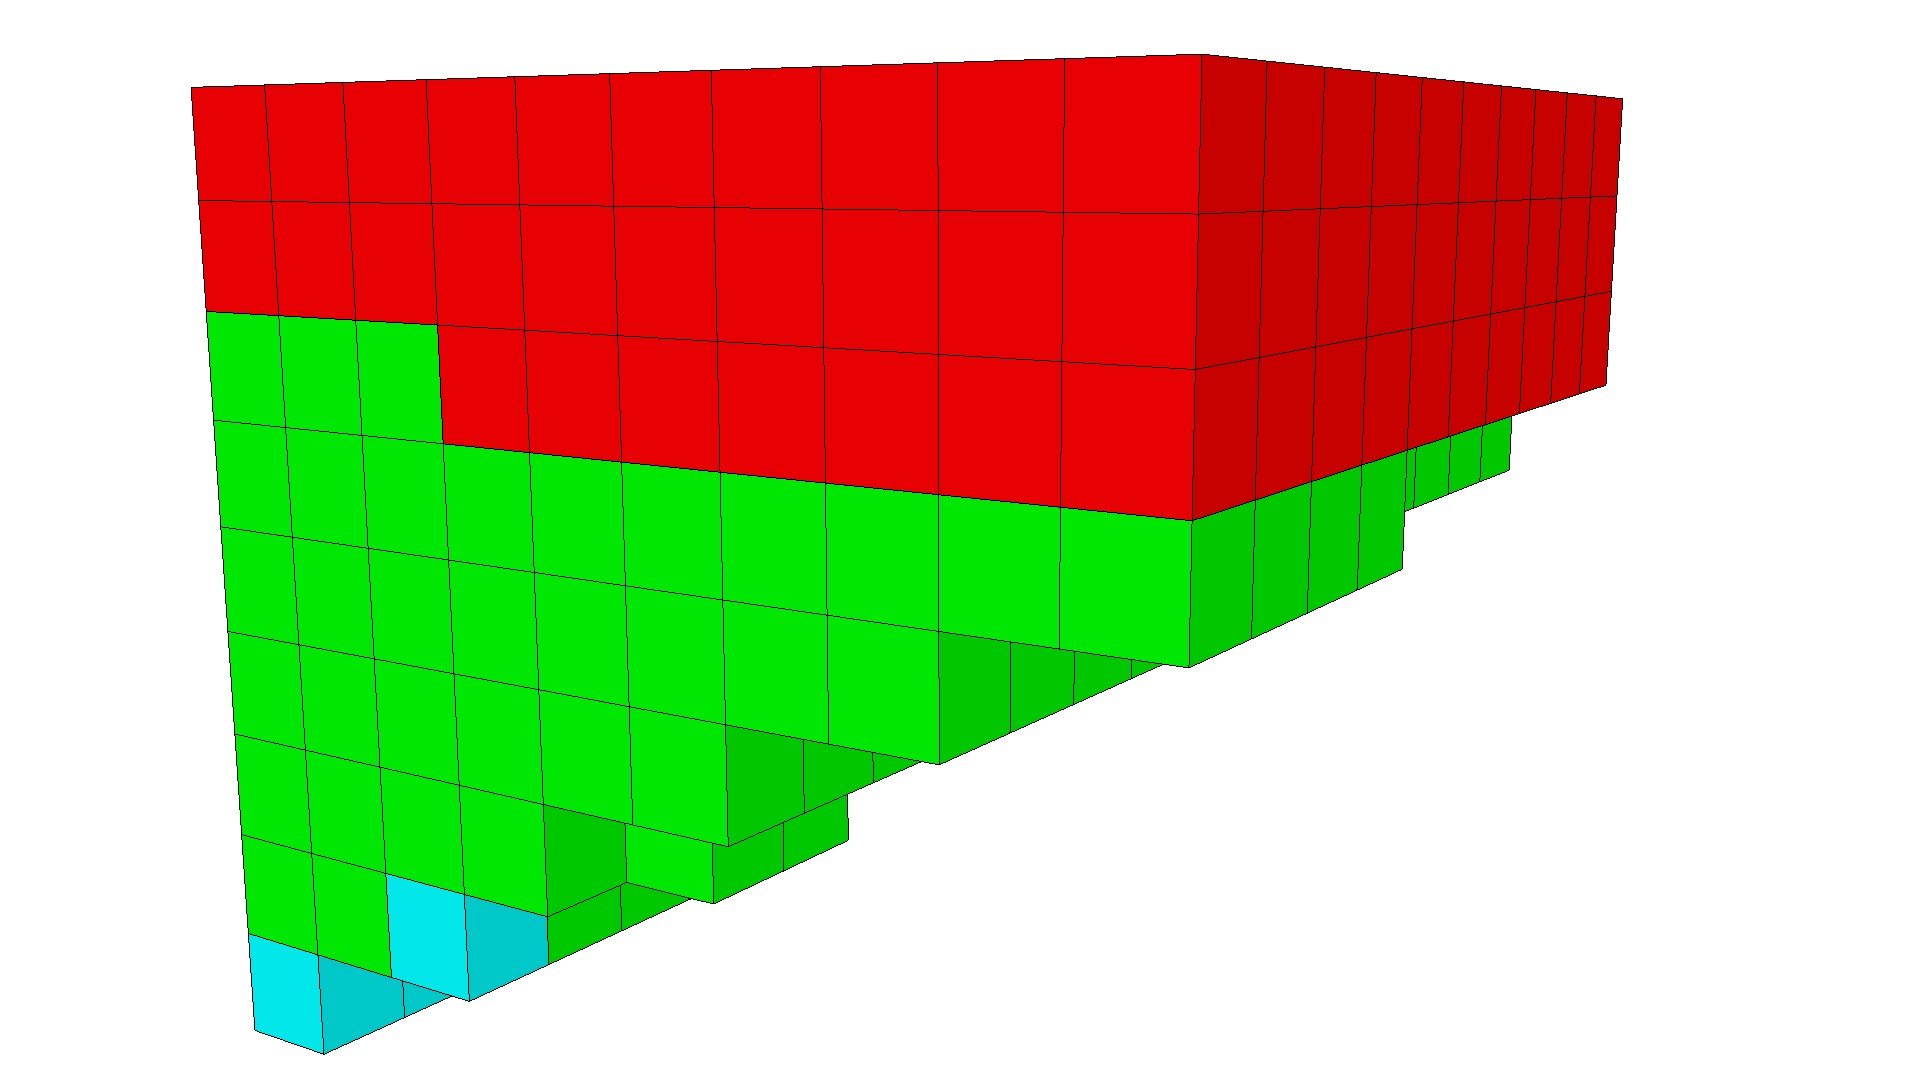
\includegraphics[width=0.19\textwidth]{../Figures/Robots/f_4_g_500.jpg}\\
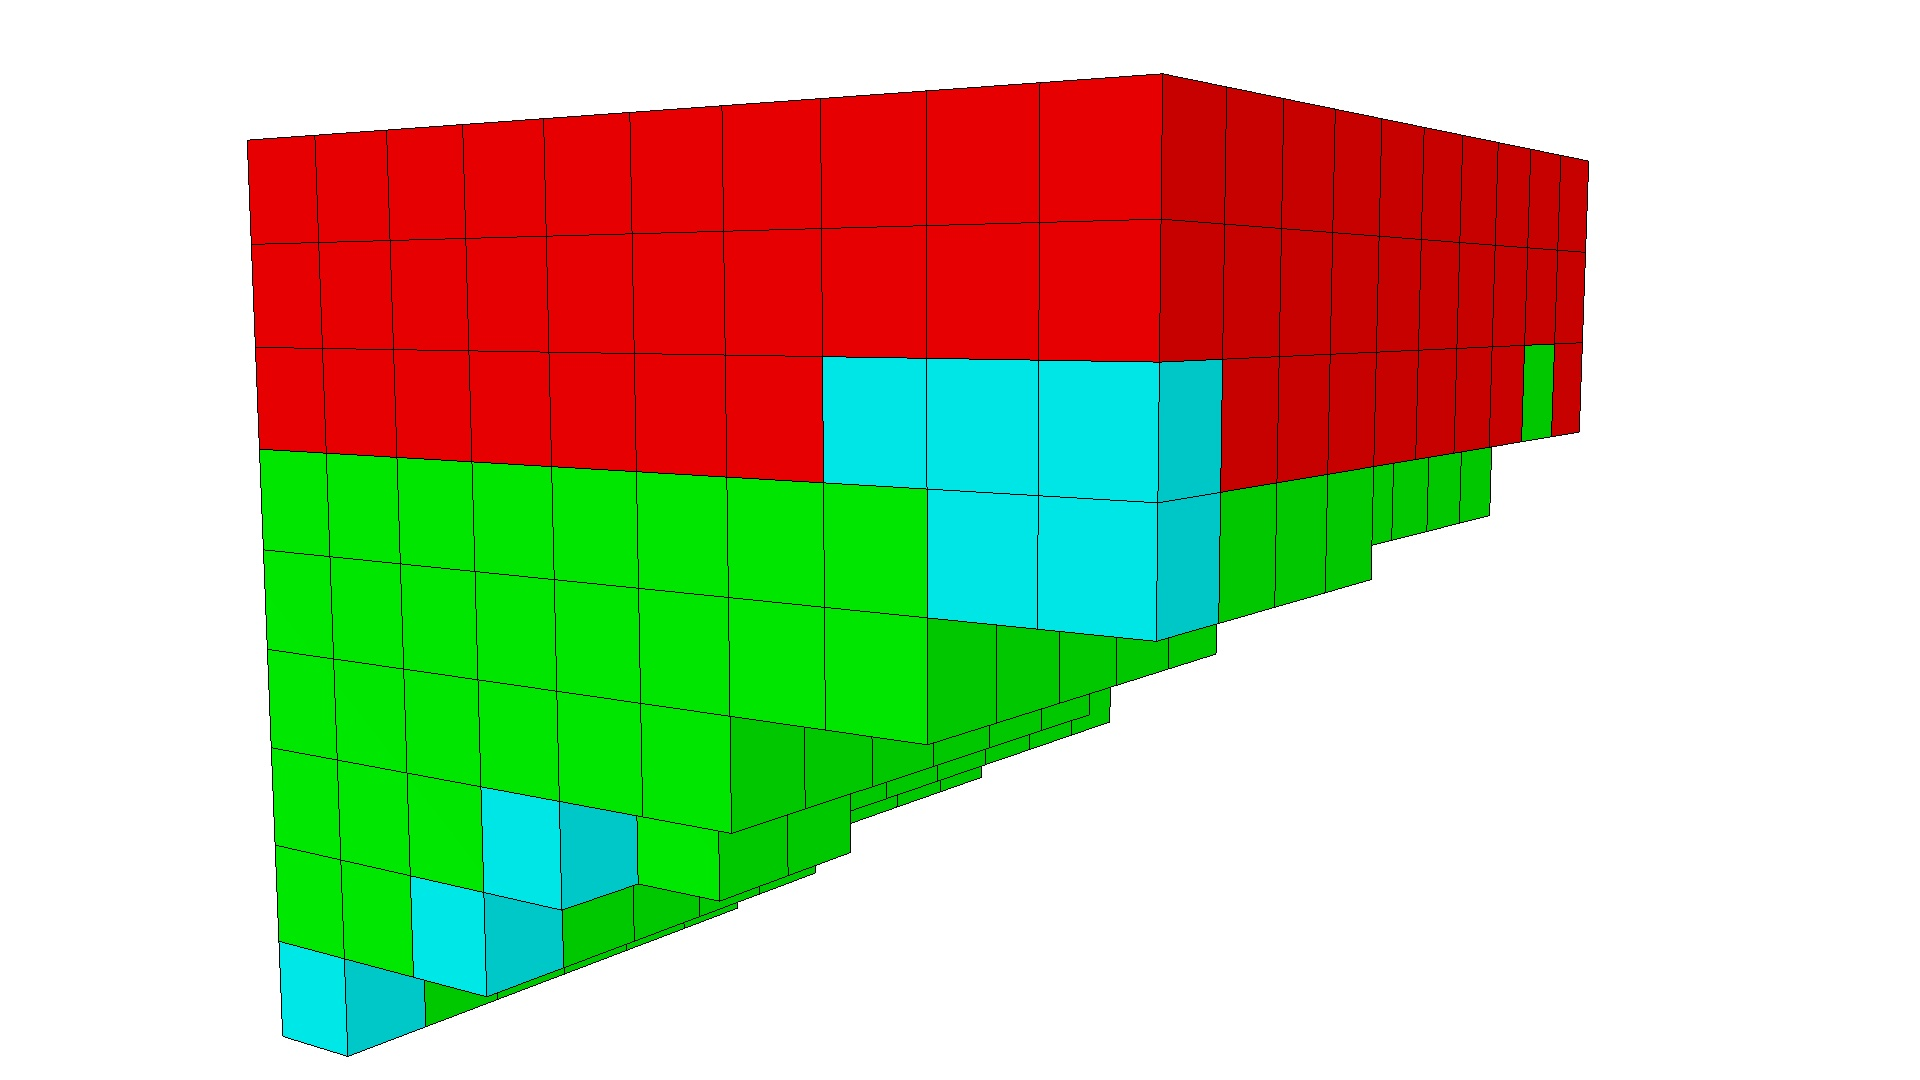
\includegraphics[width=0.19\textwidth]{../Figures/Robots/f_4_g_600.jpg}
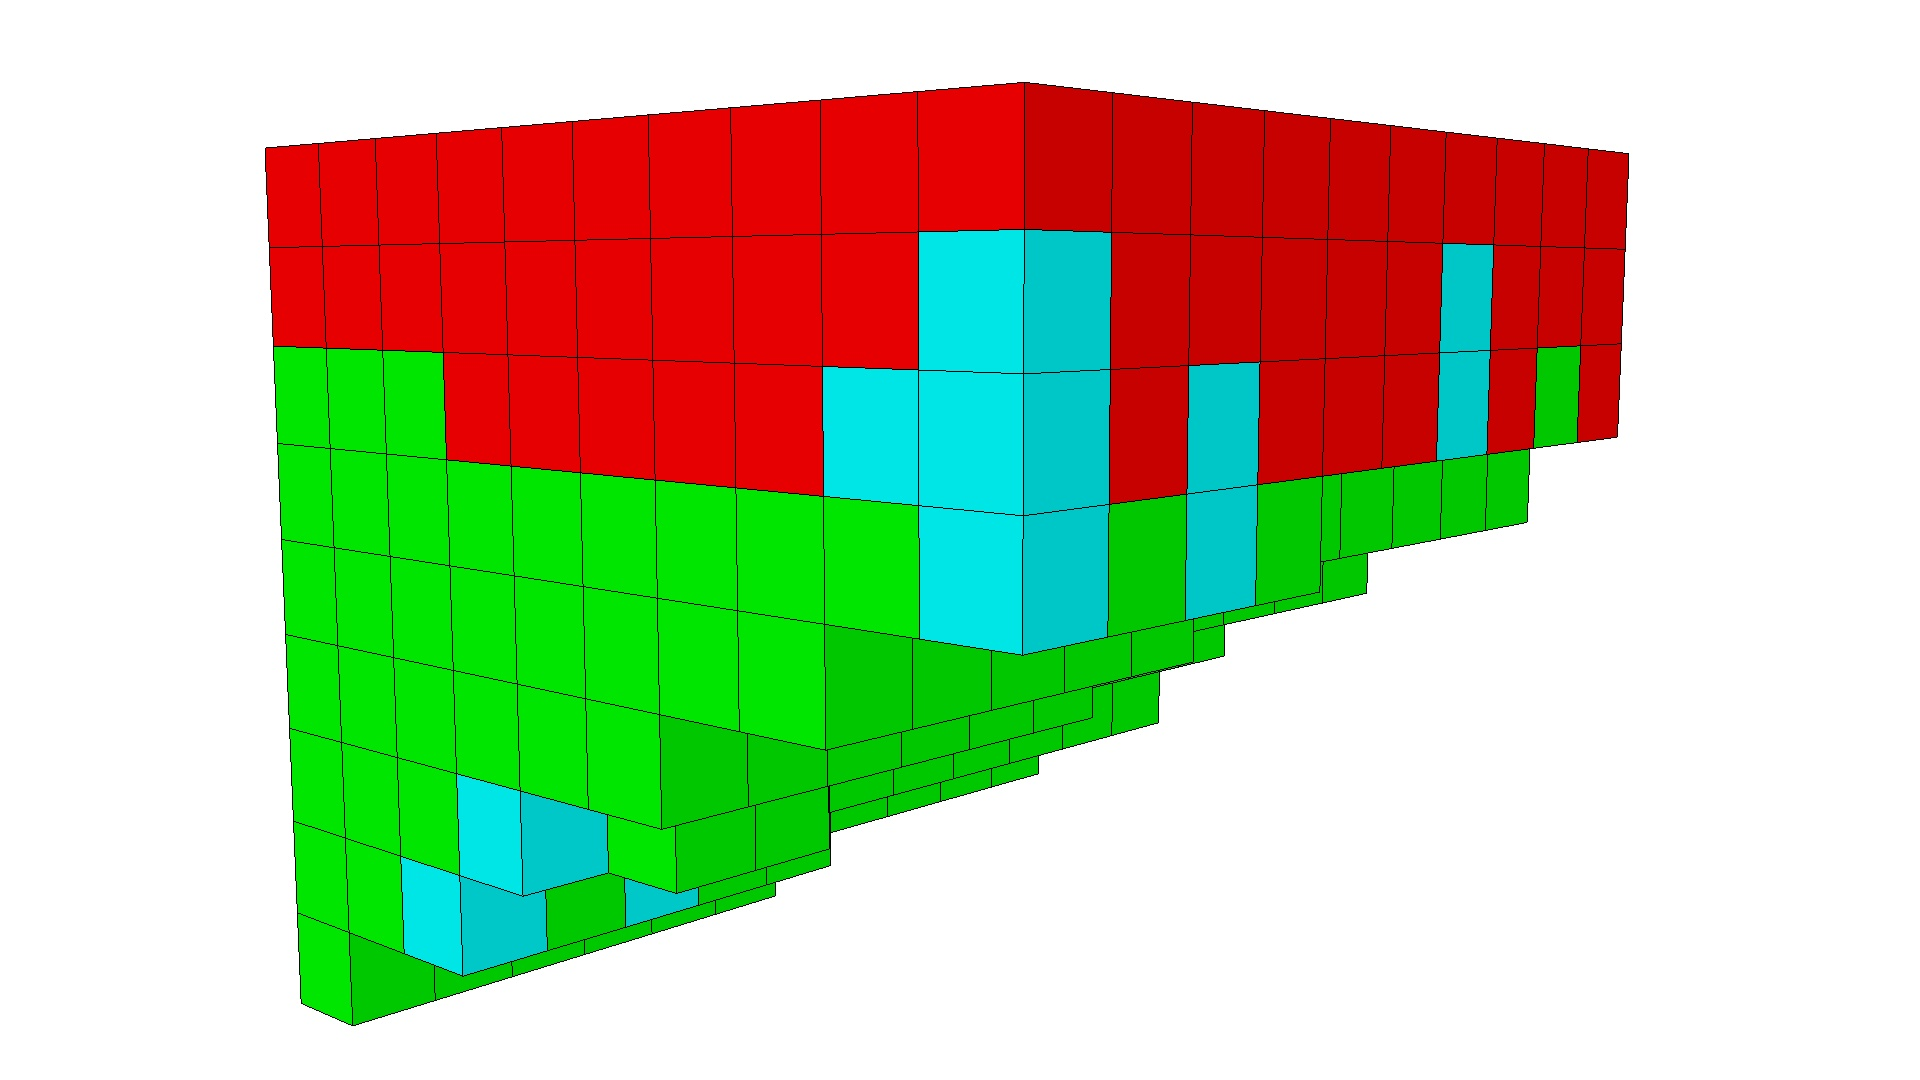
\includegraphics[width=0.19\textwidth]{../Figures/Robots/f_4_g_700.jpg}
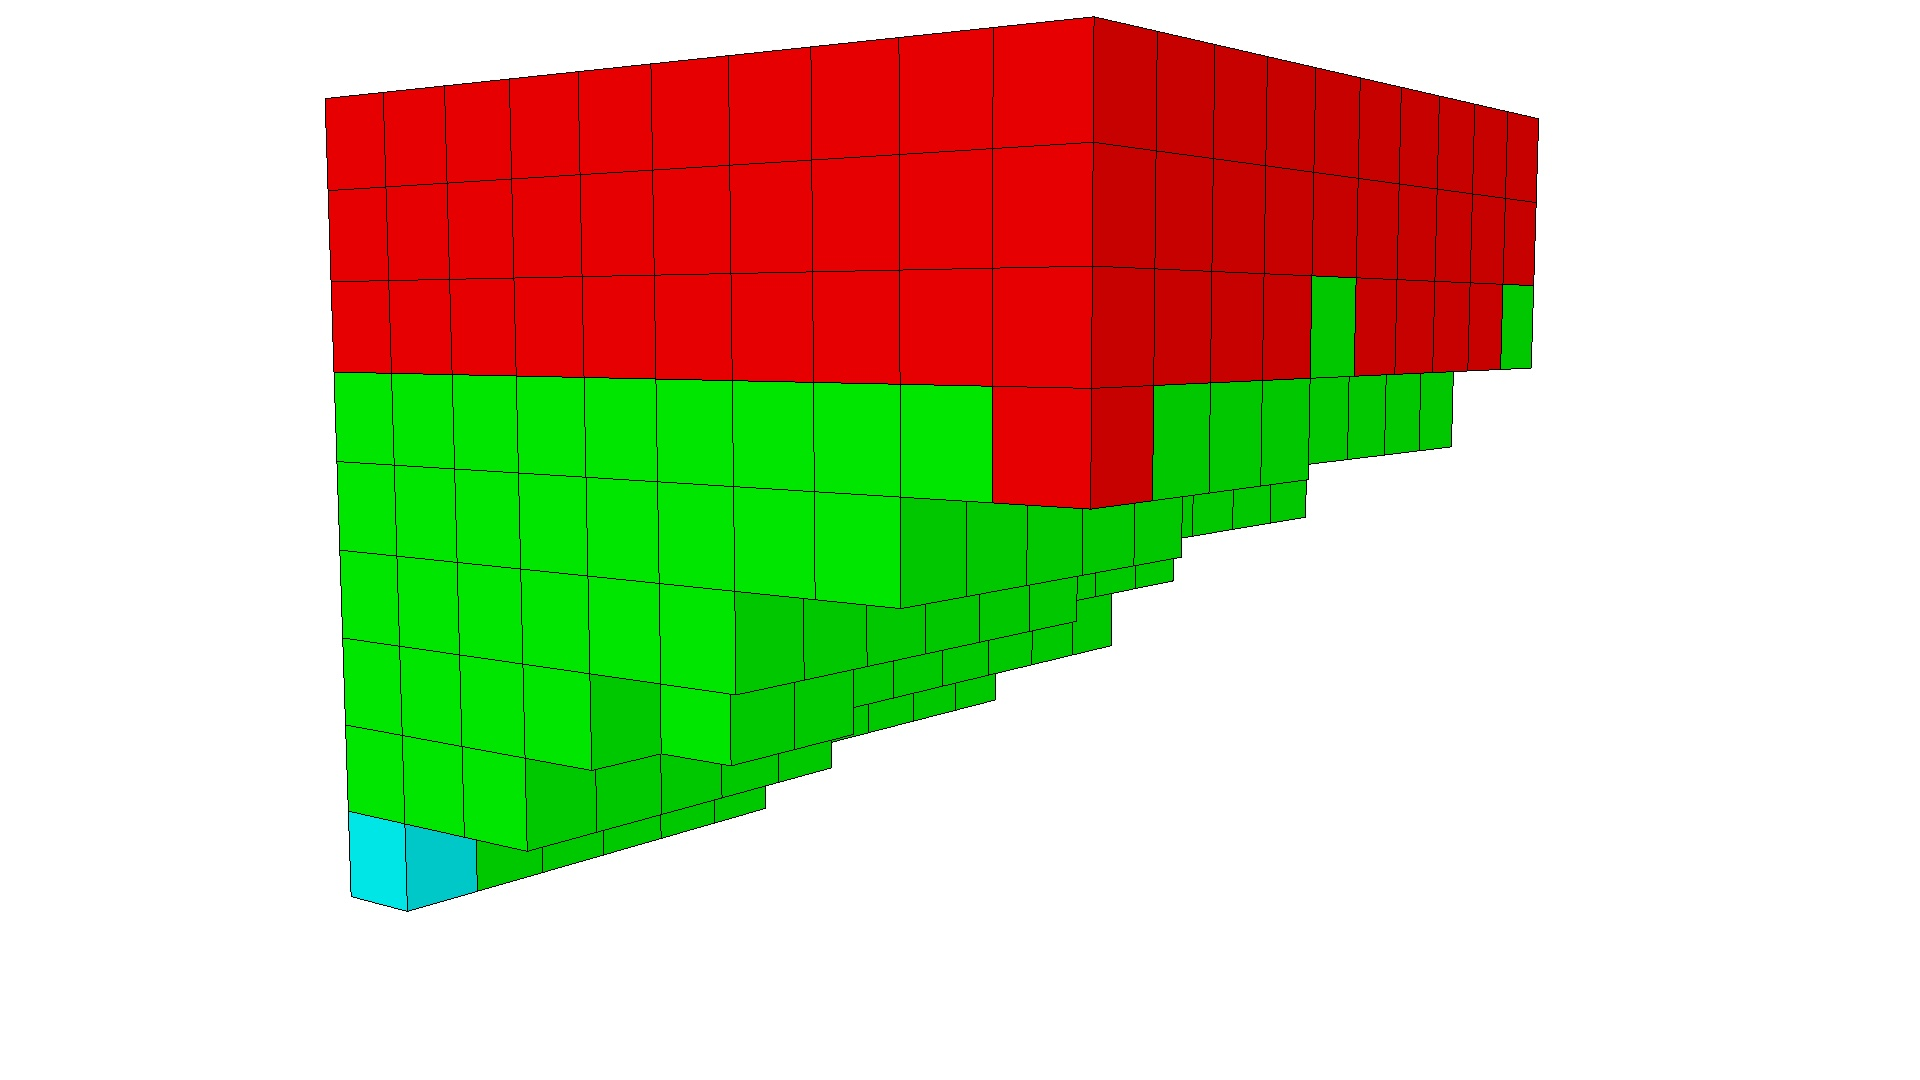
\includegraphics[width=0.19\textwidth]{../Figures/Robots/f_4_g_800.jpg}
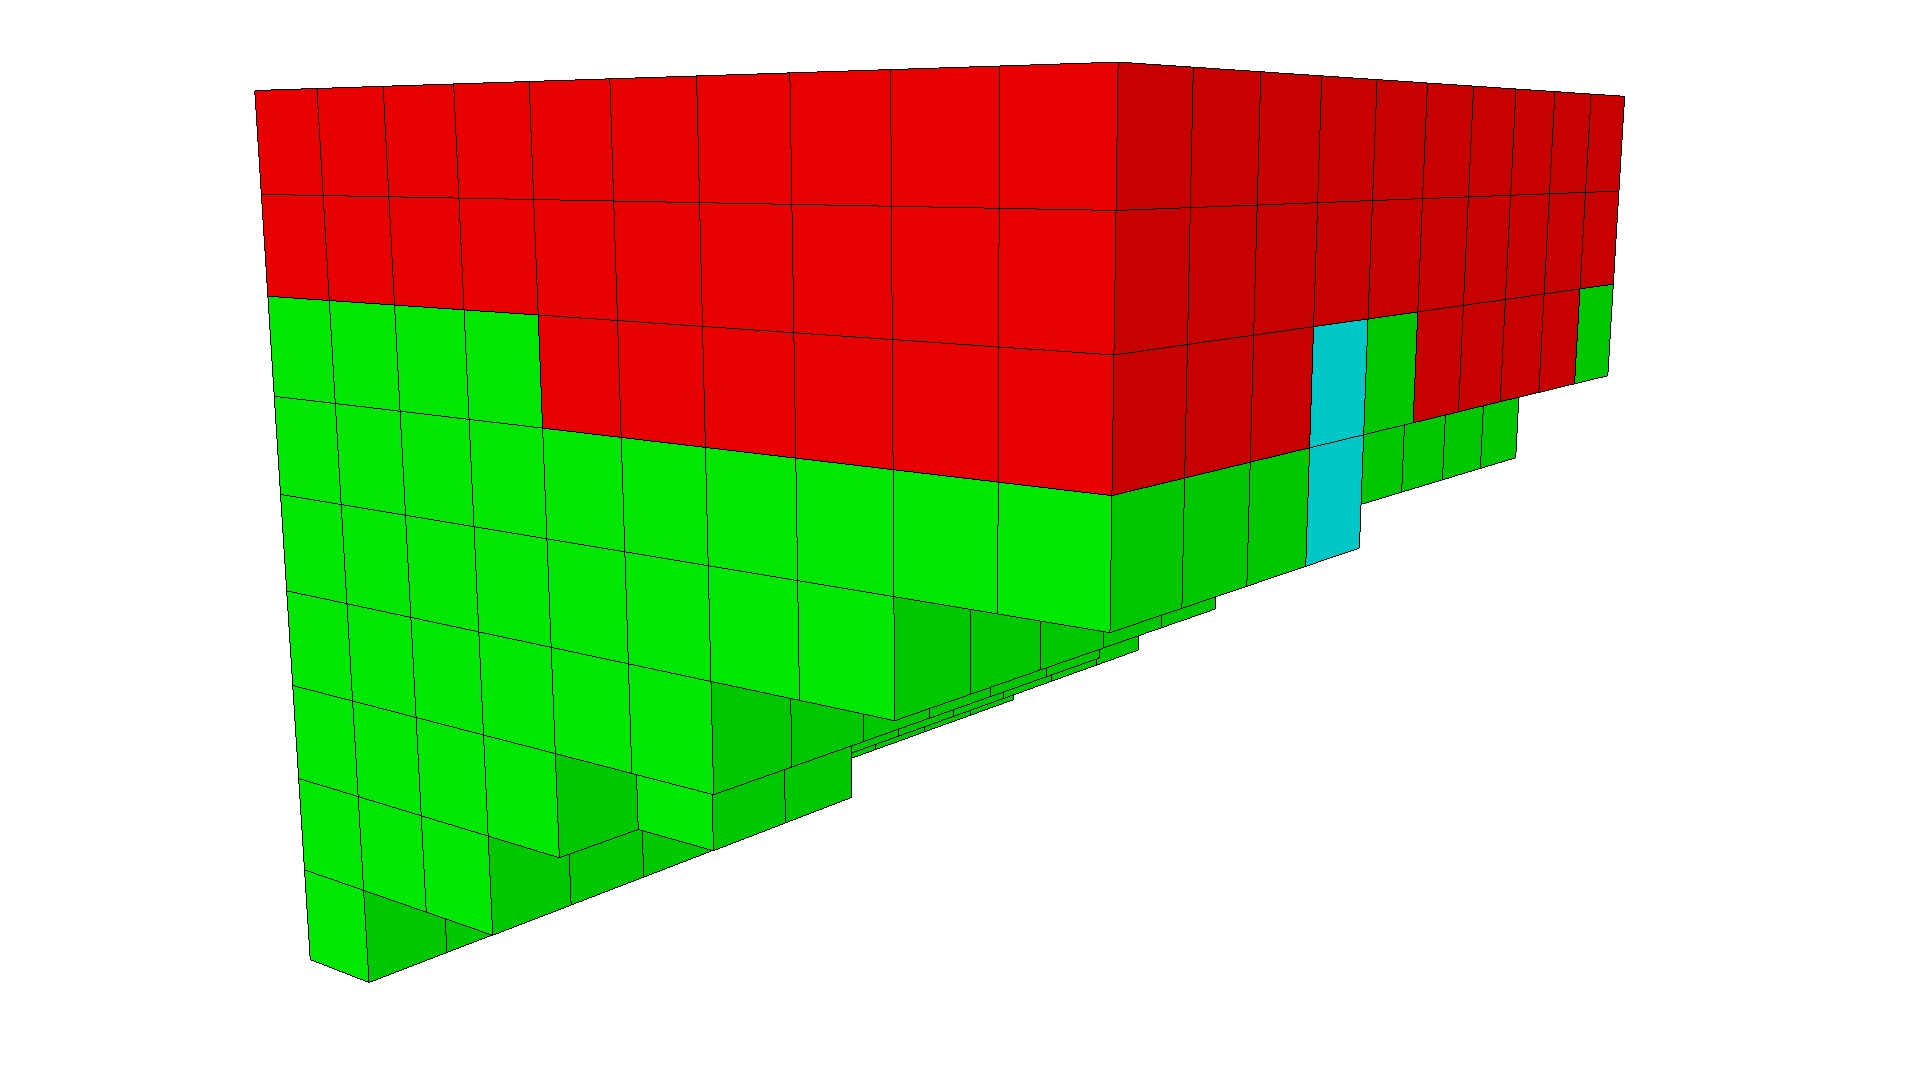
\includegraphics[width=0.19\textwidth]{../Figures/Robots/f_4_g_900.jpg}
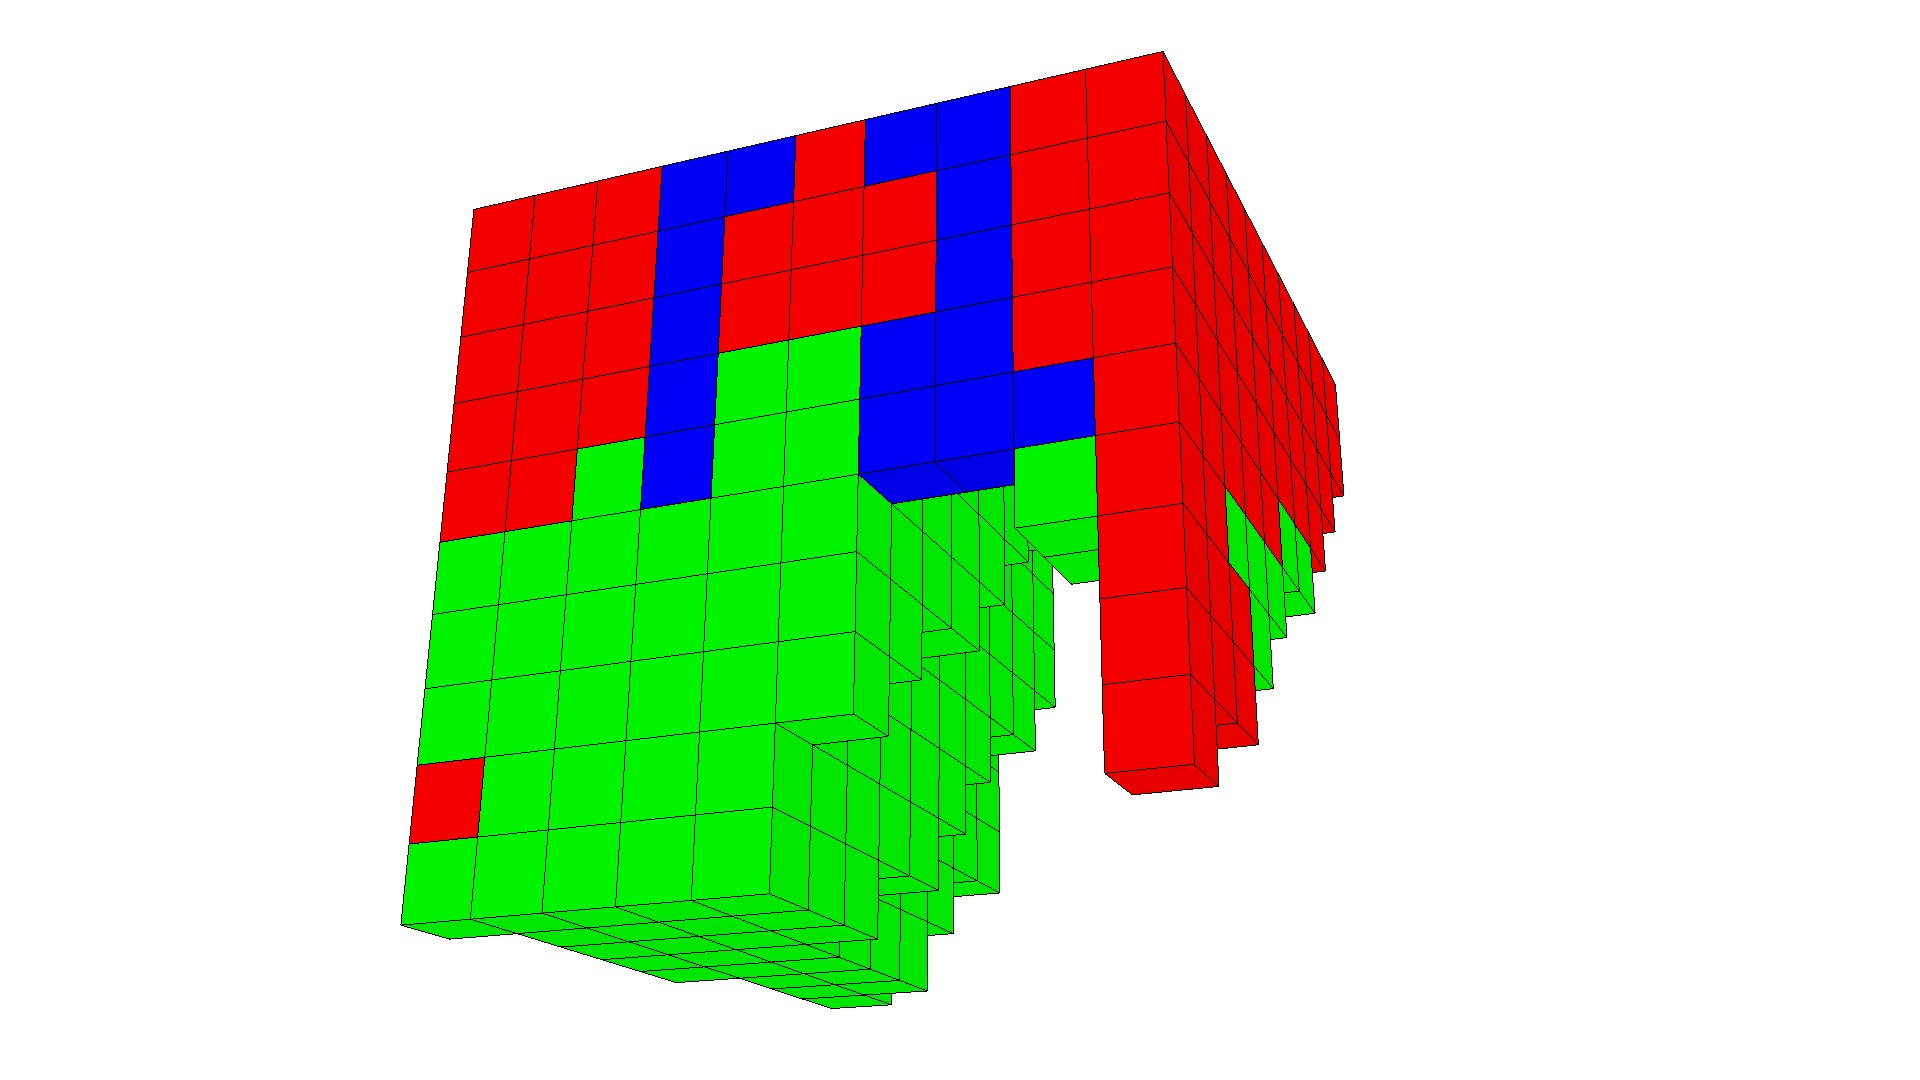
\includegraphics[width=0.19\textwidth]{../Figures/Robots/f_4_g_1000.jpg}
\caption{Fitness based search}
\end{subfigure}\\
\begin{subfigure}[b]{1.0\textwidth}
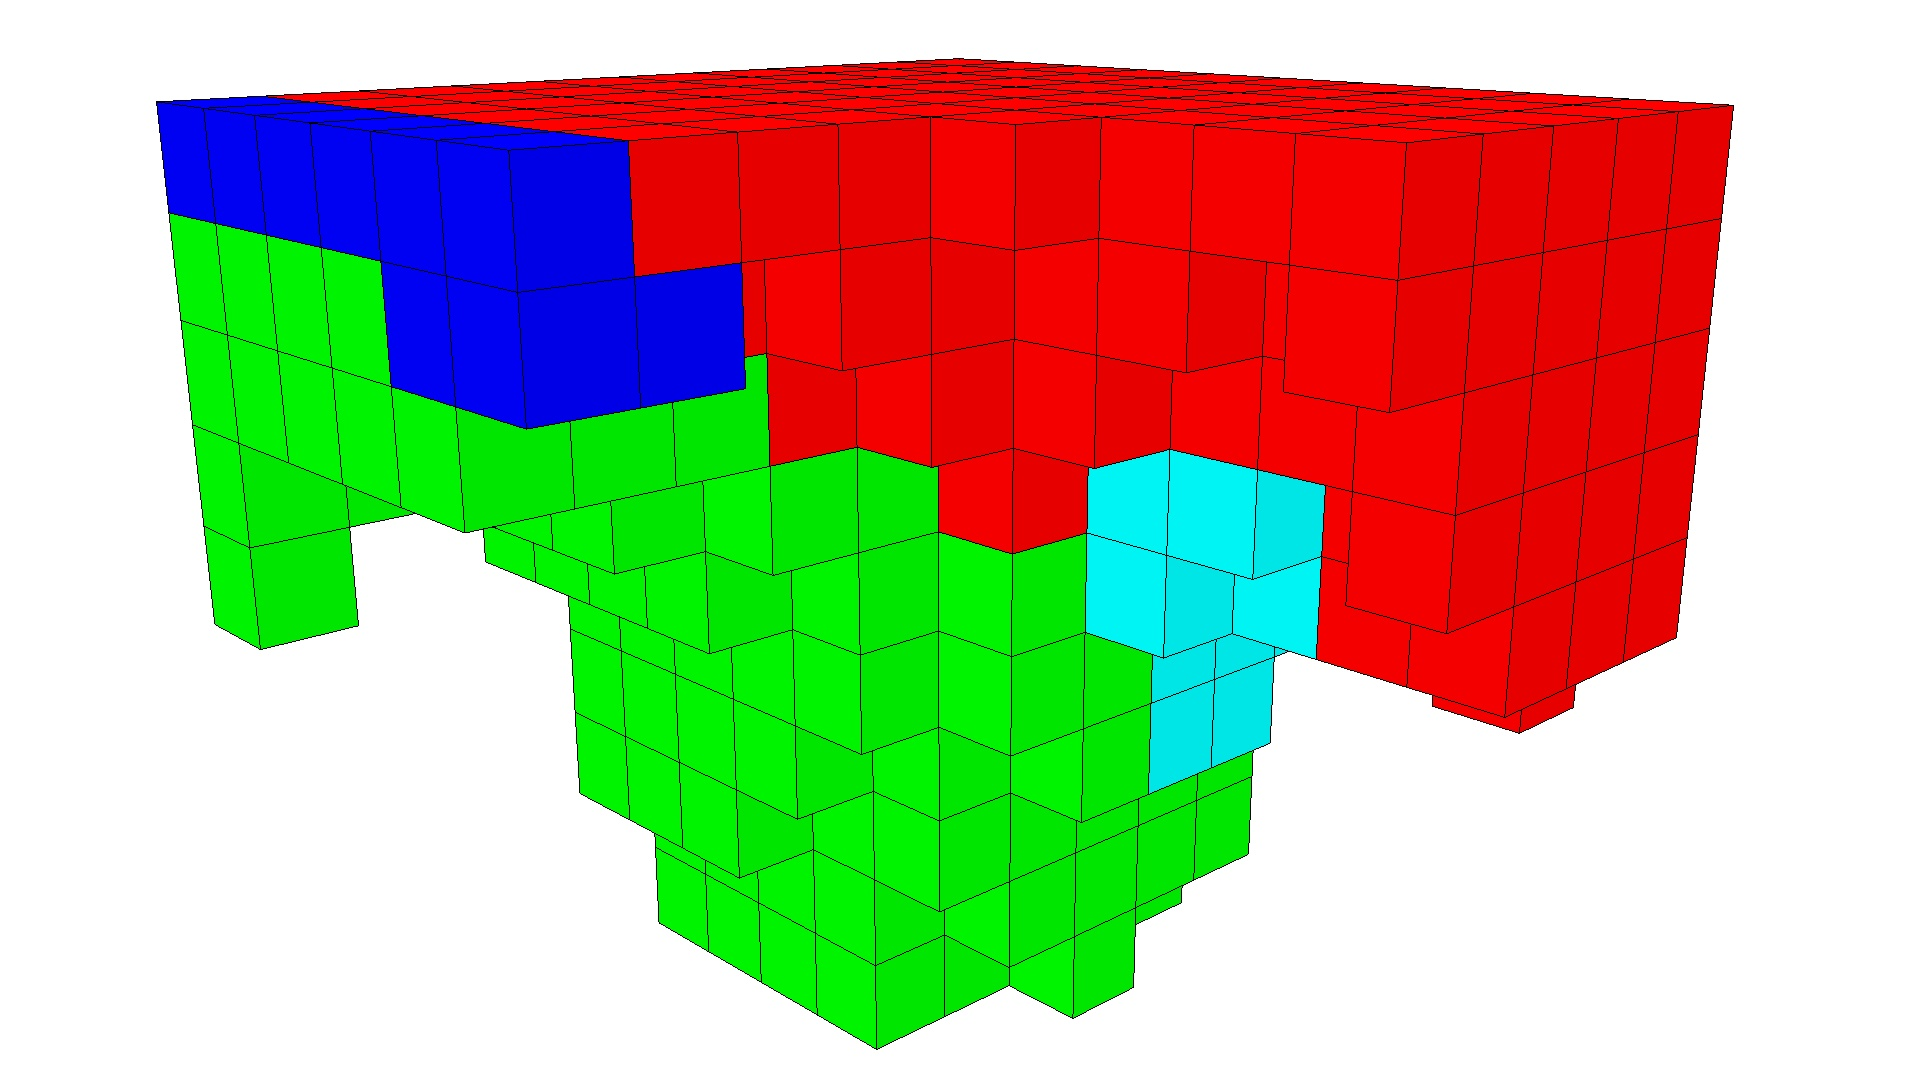
\includegraphics[width=0.19\textwidth]{../Figures/Robots/n_4_g_100.jpg}
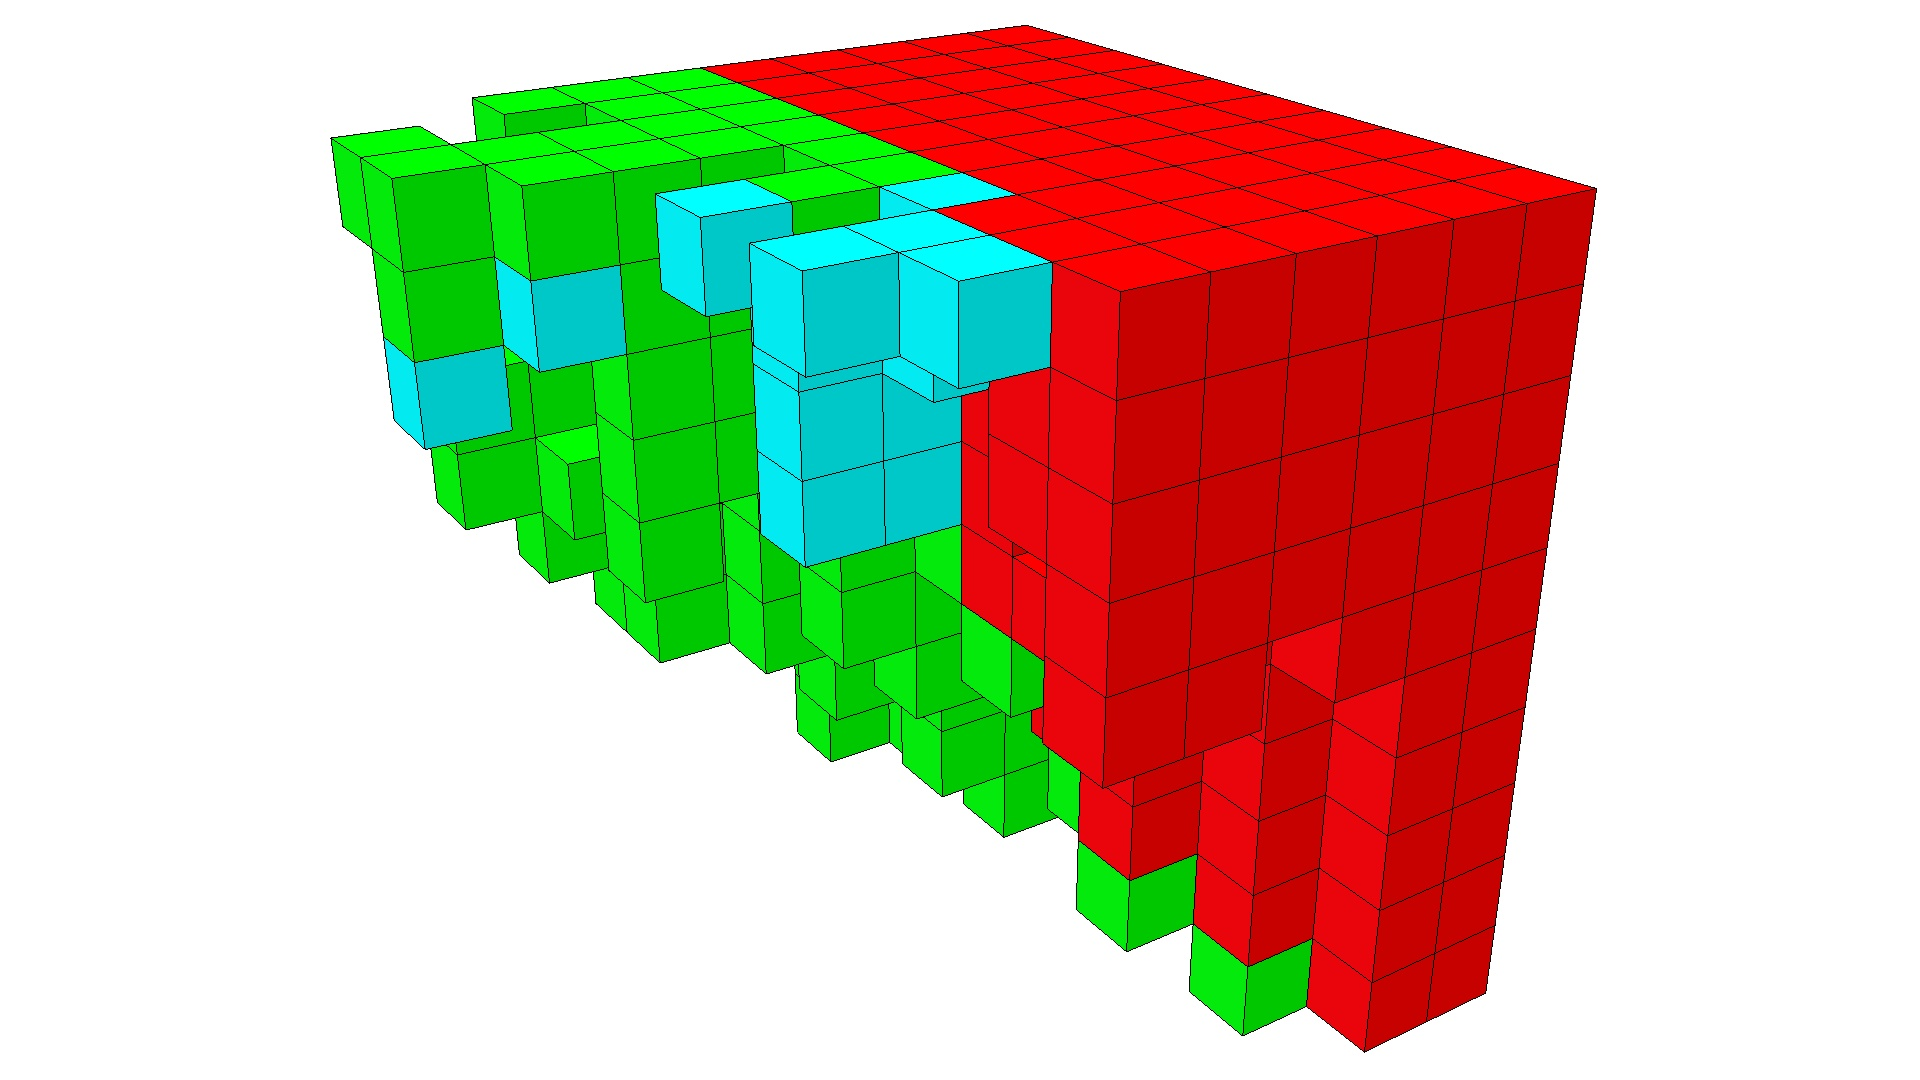
\includegraphics[width=0.19\textwidth]{../Figures/Robots/n_4_g_200.jpg}
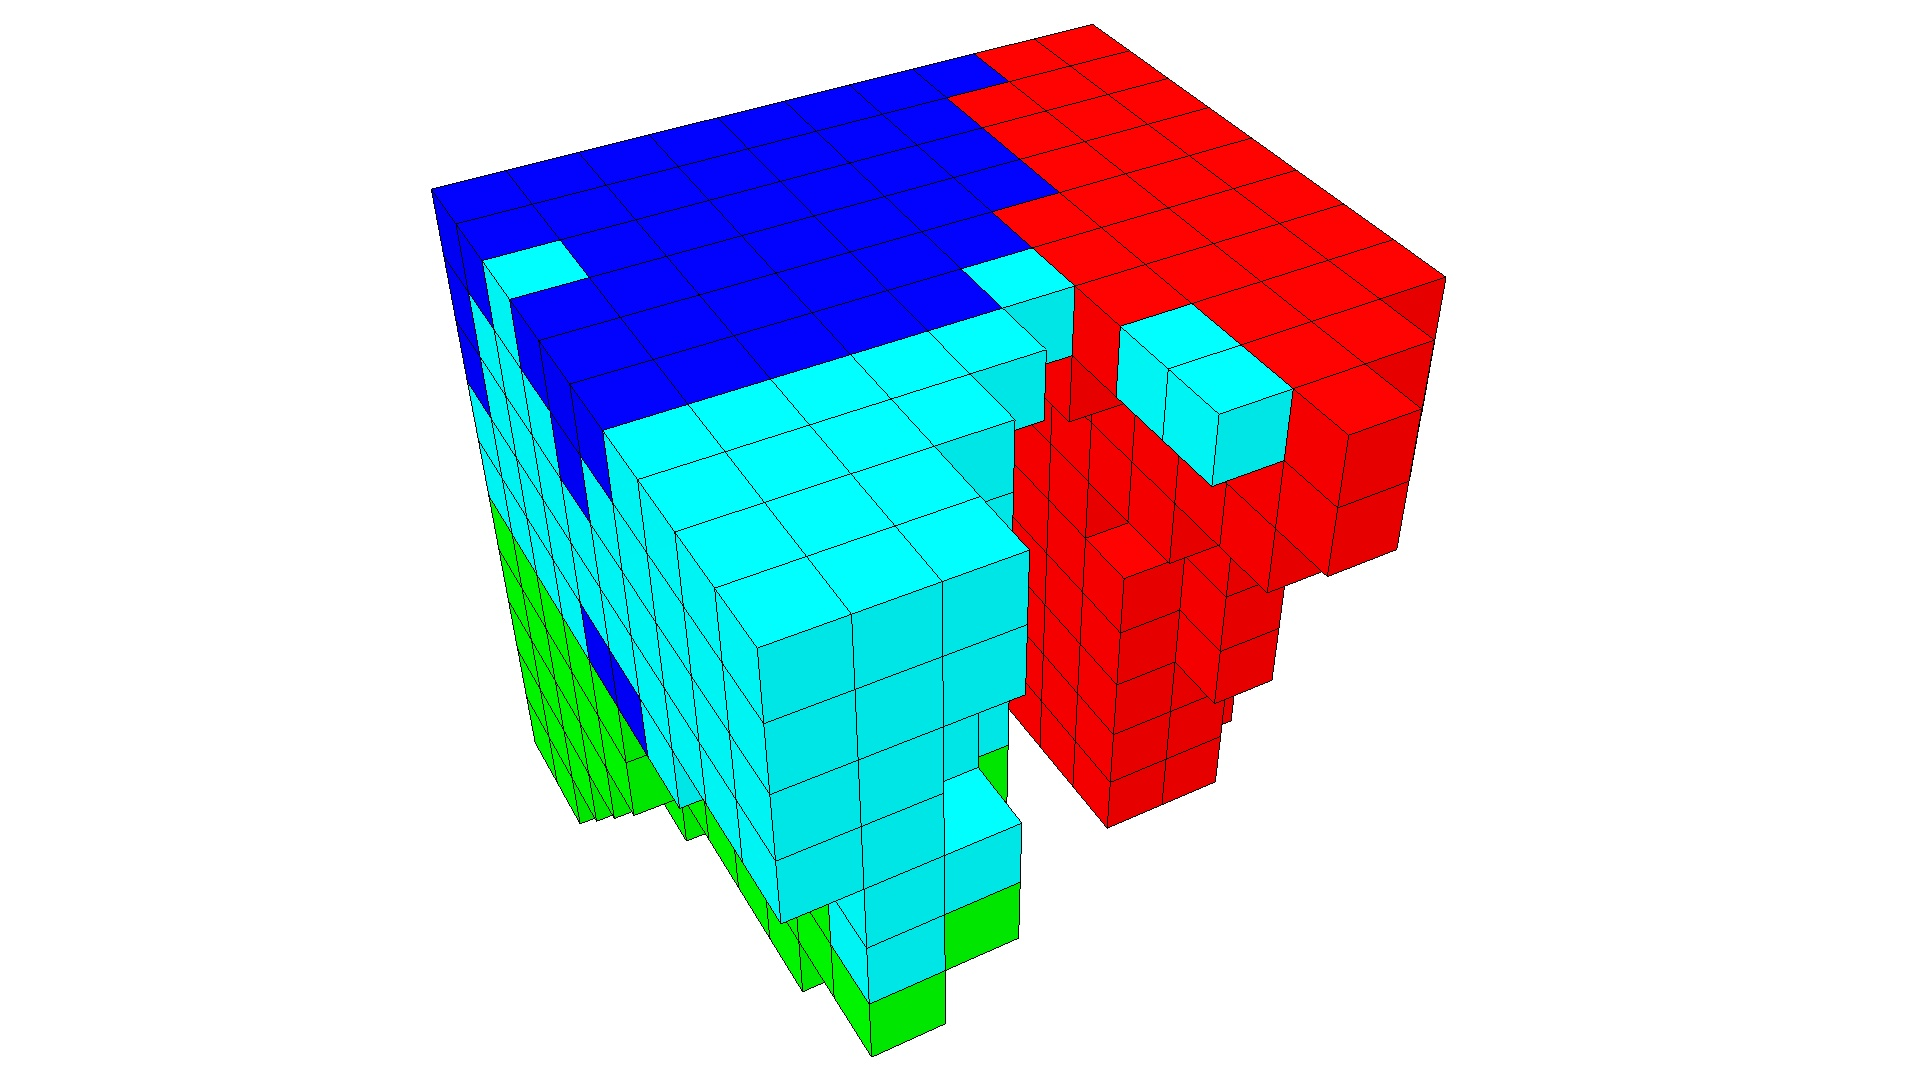
\includegraphics[width=0.19\textwidth]{../Figures/Robots/n_4_g_300.jpg}
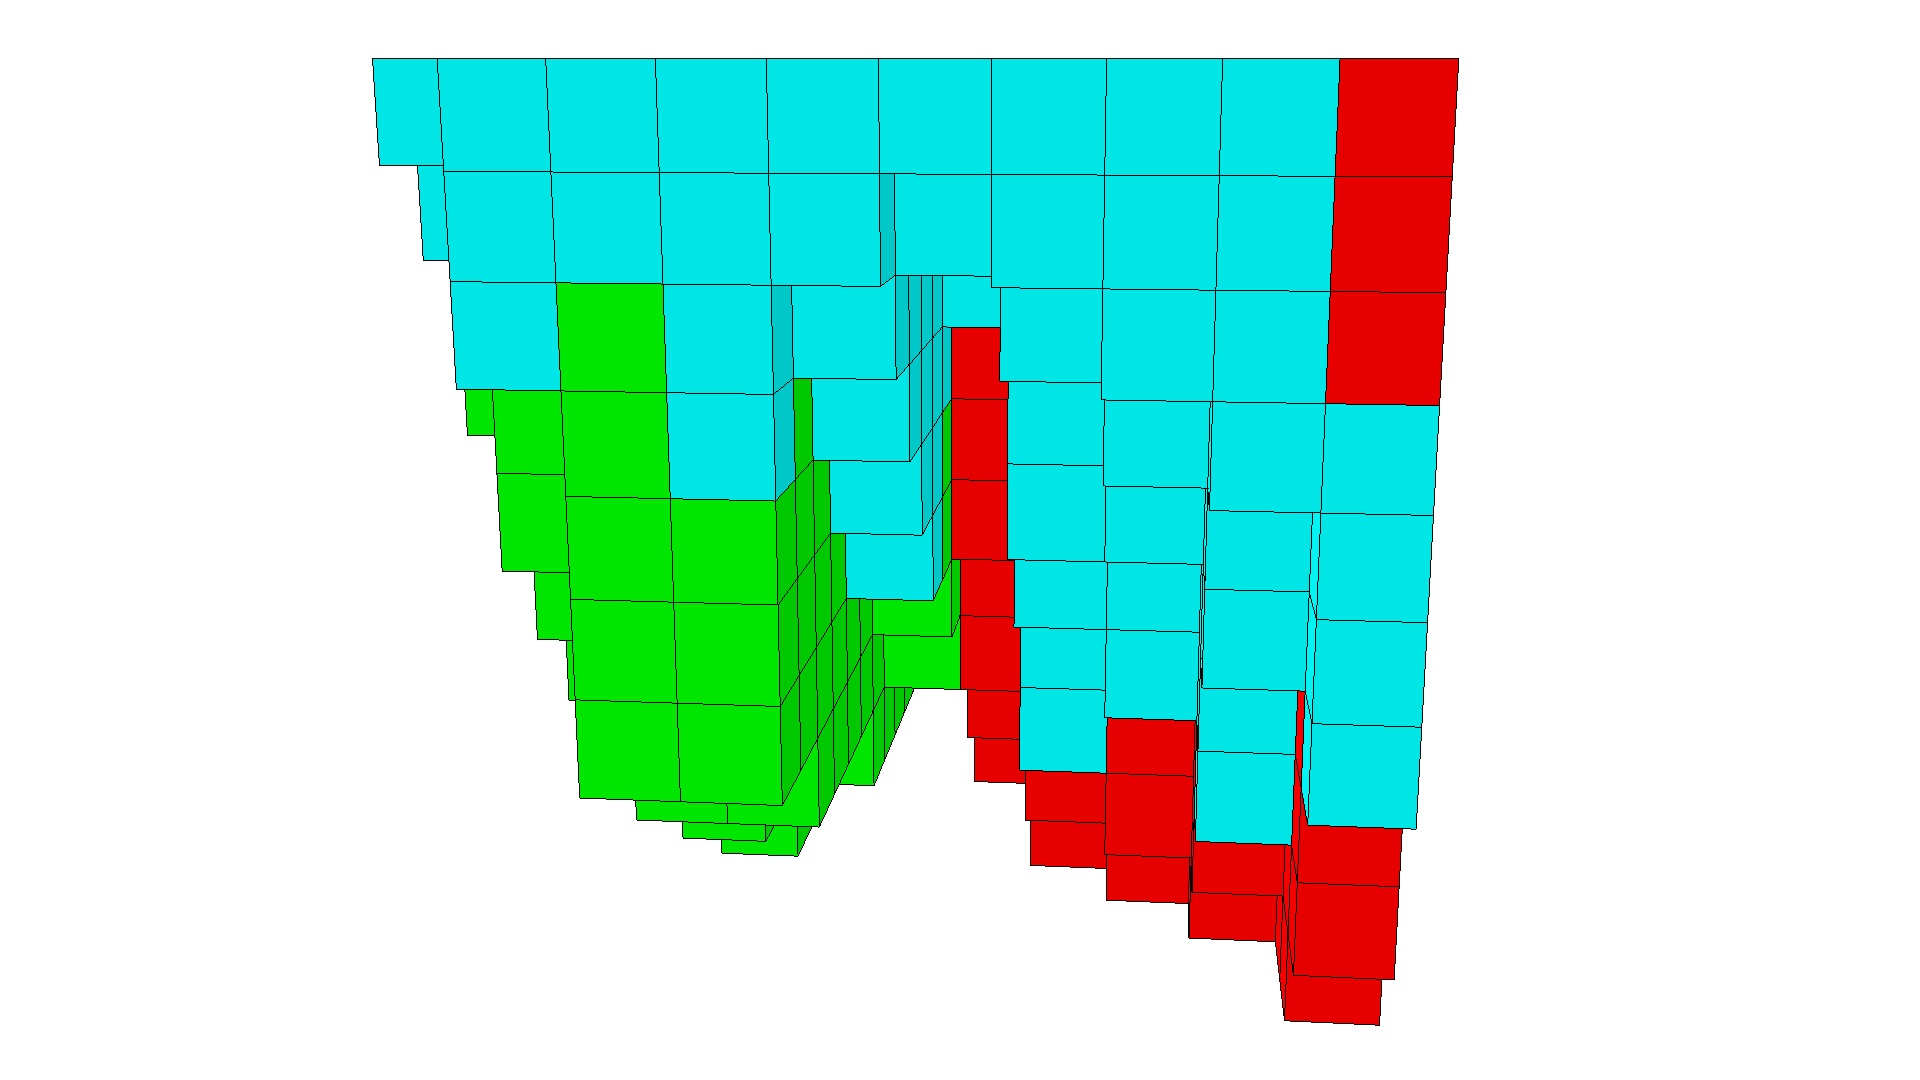
\includegraphics[width=0.19\textwidth]{../Figures/Robots/n_4_g_400.jpg}
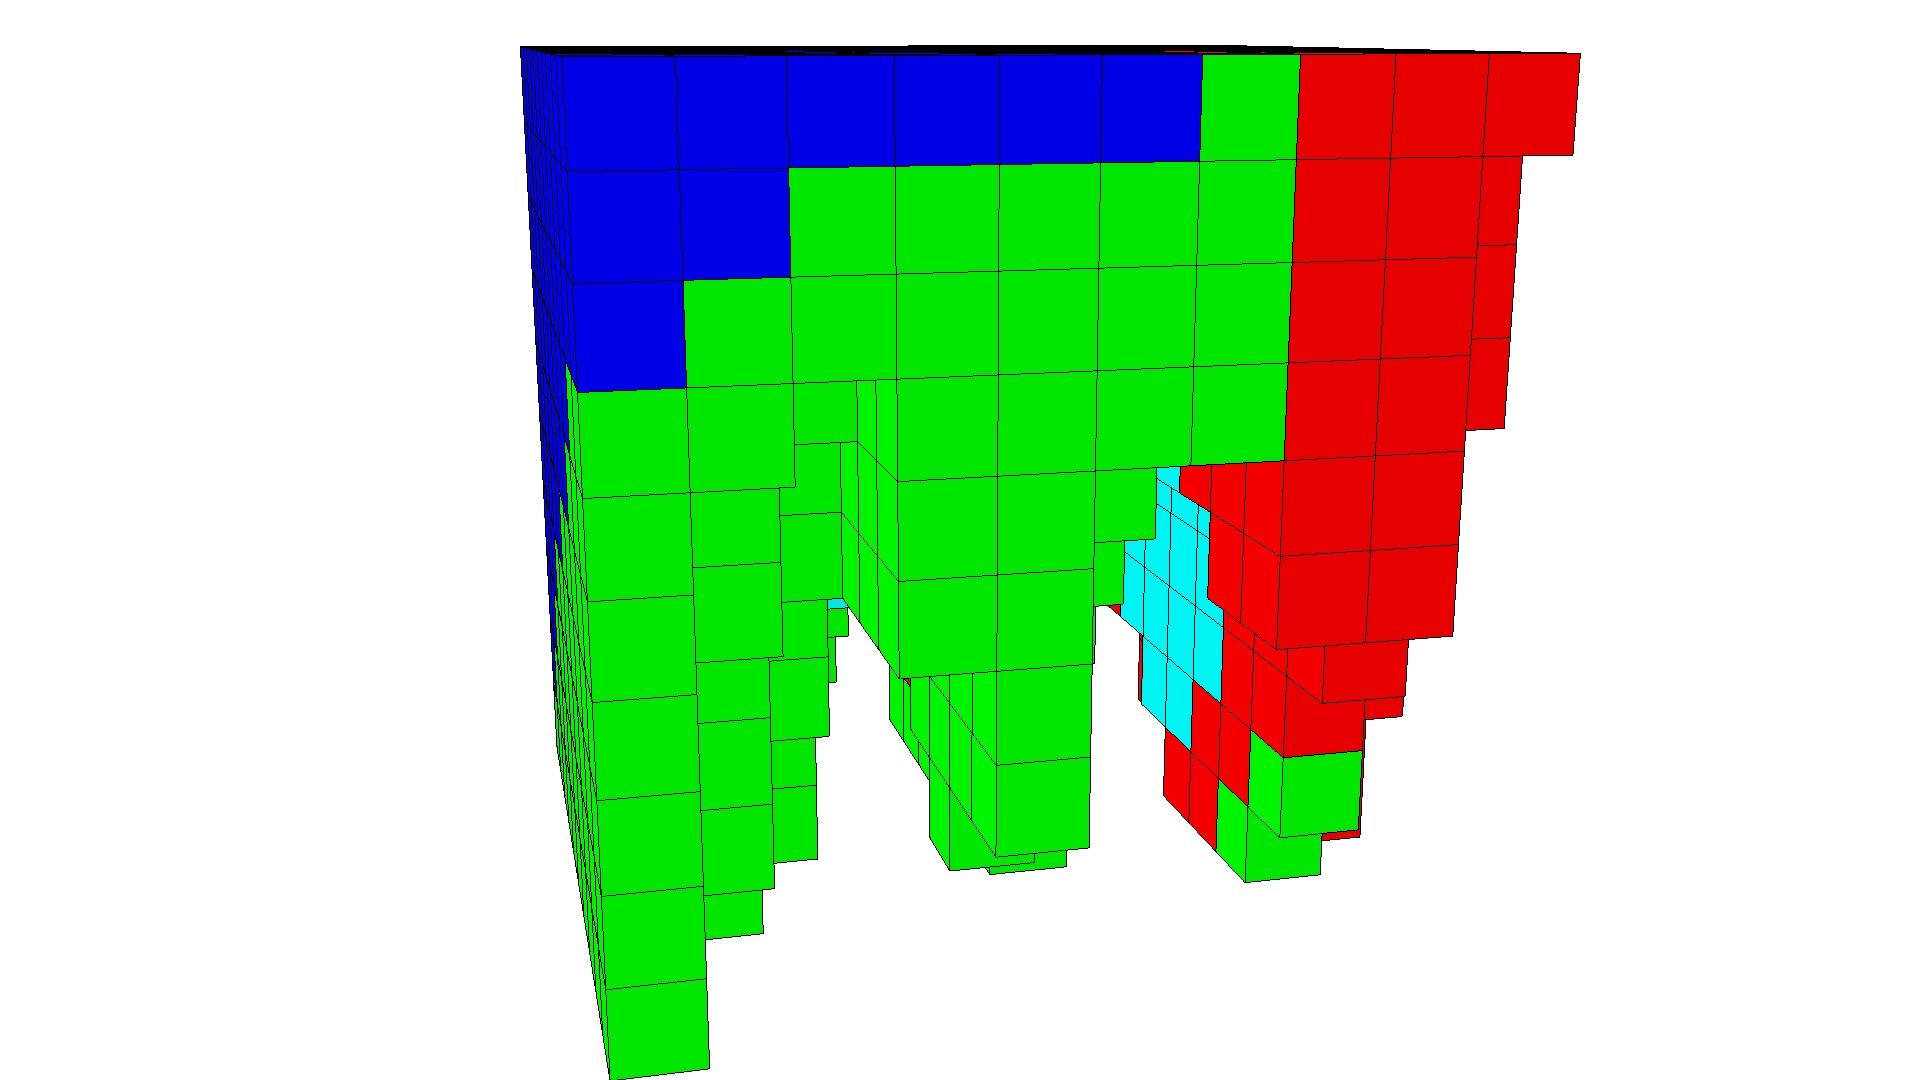
\includegraphics[width=0.19\textwidth]{../Figures/Robots/n_4_g_500.jpg}\\
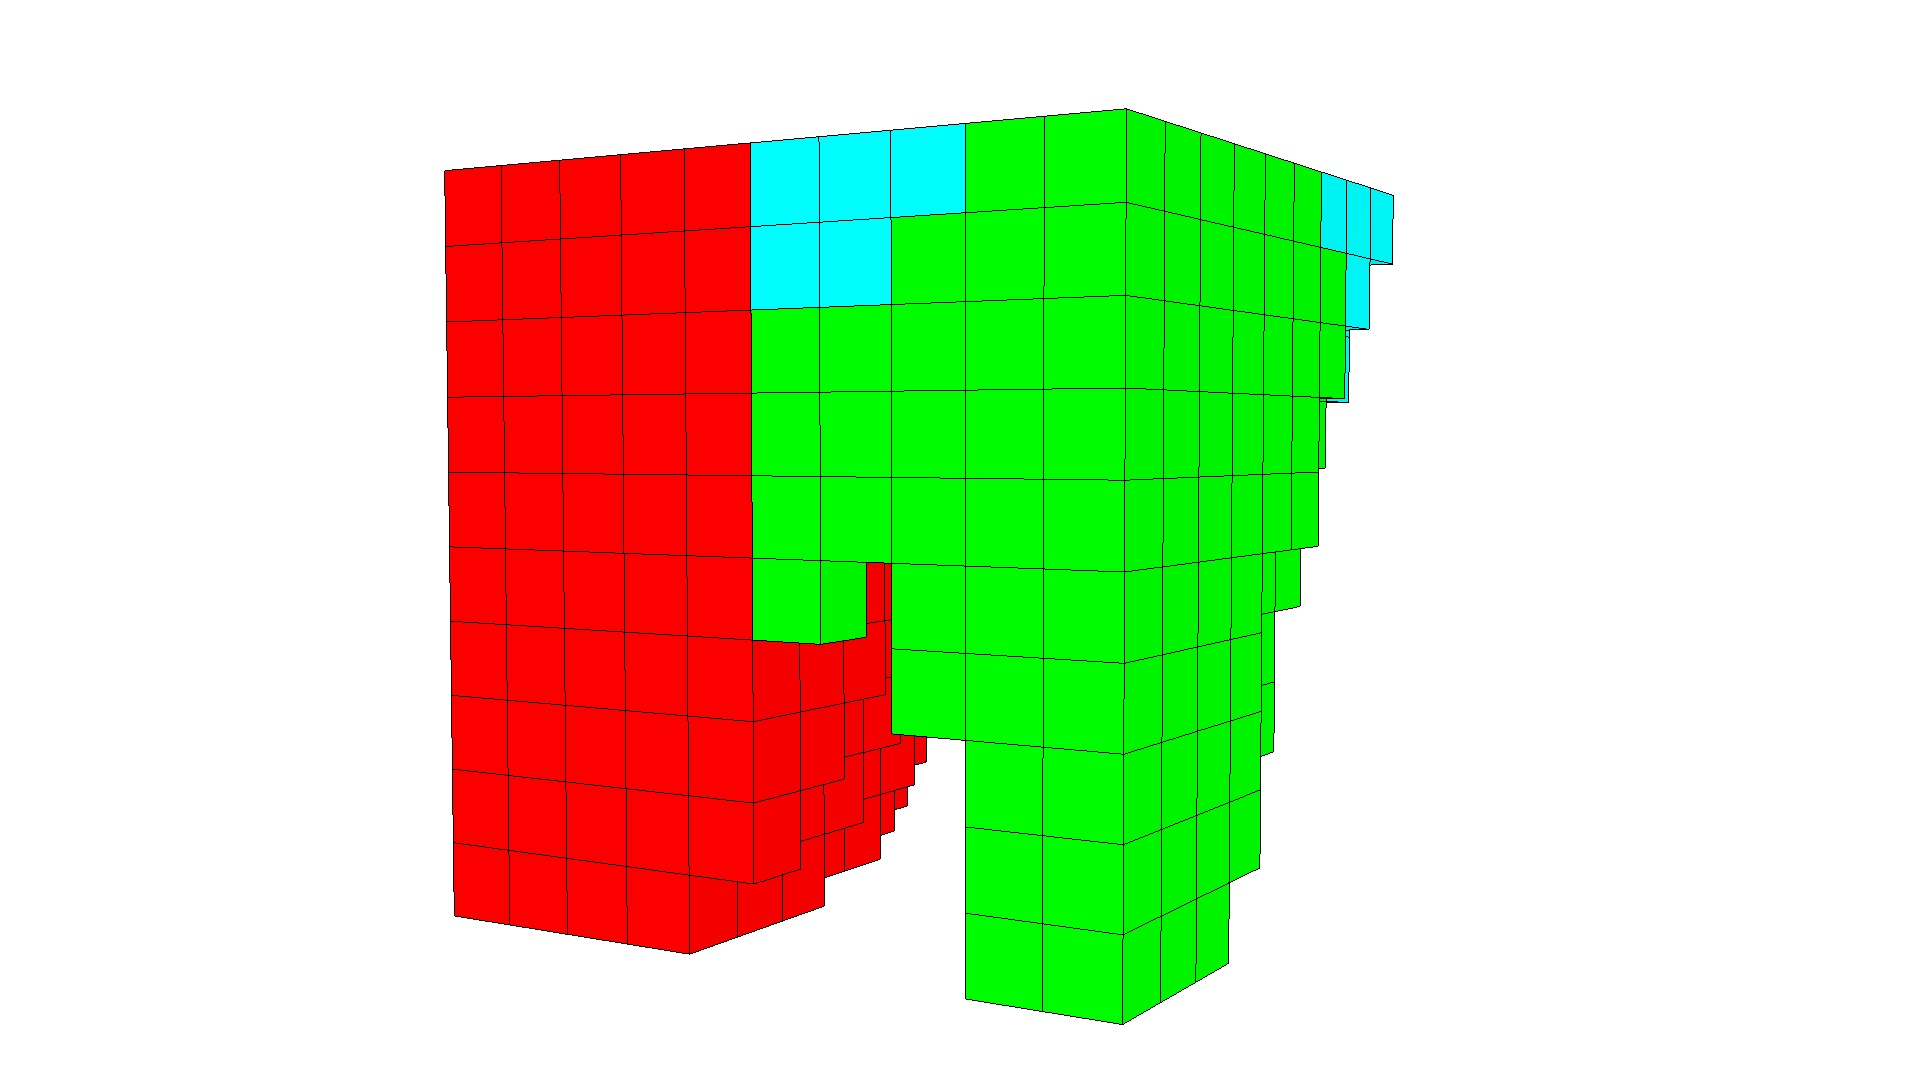
\includegraphics[width=0.19\textwidth]{../Figures/Robots/n_4_g_600.jpg}
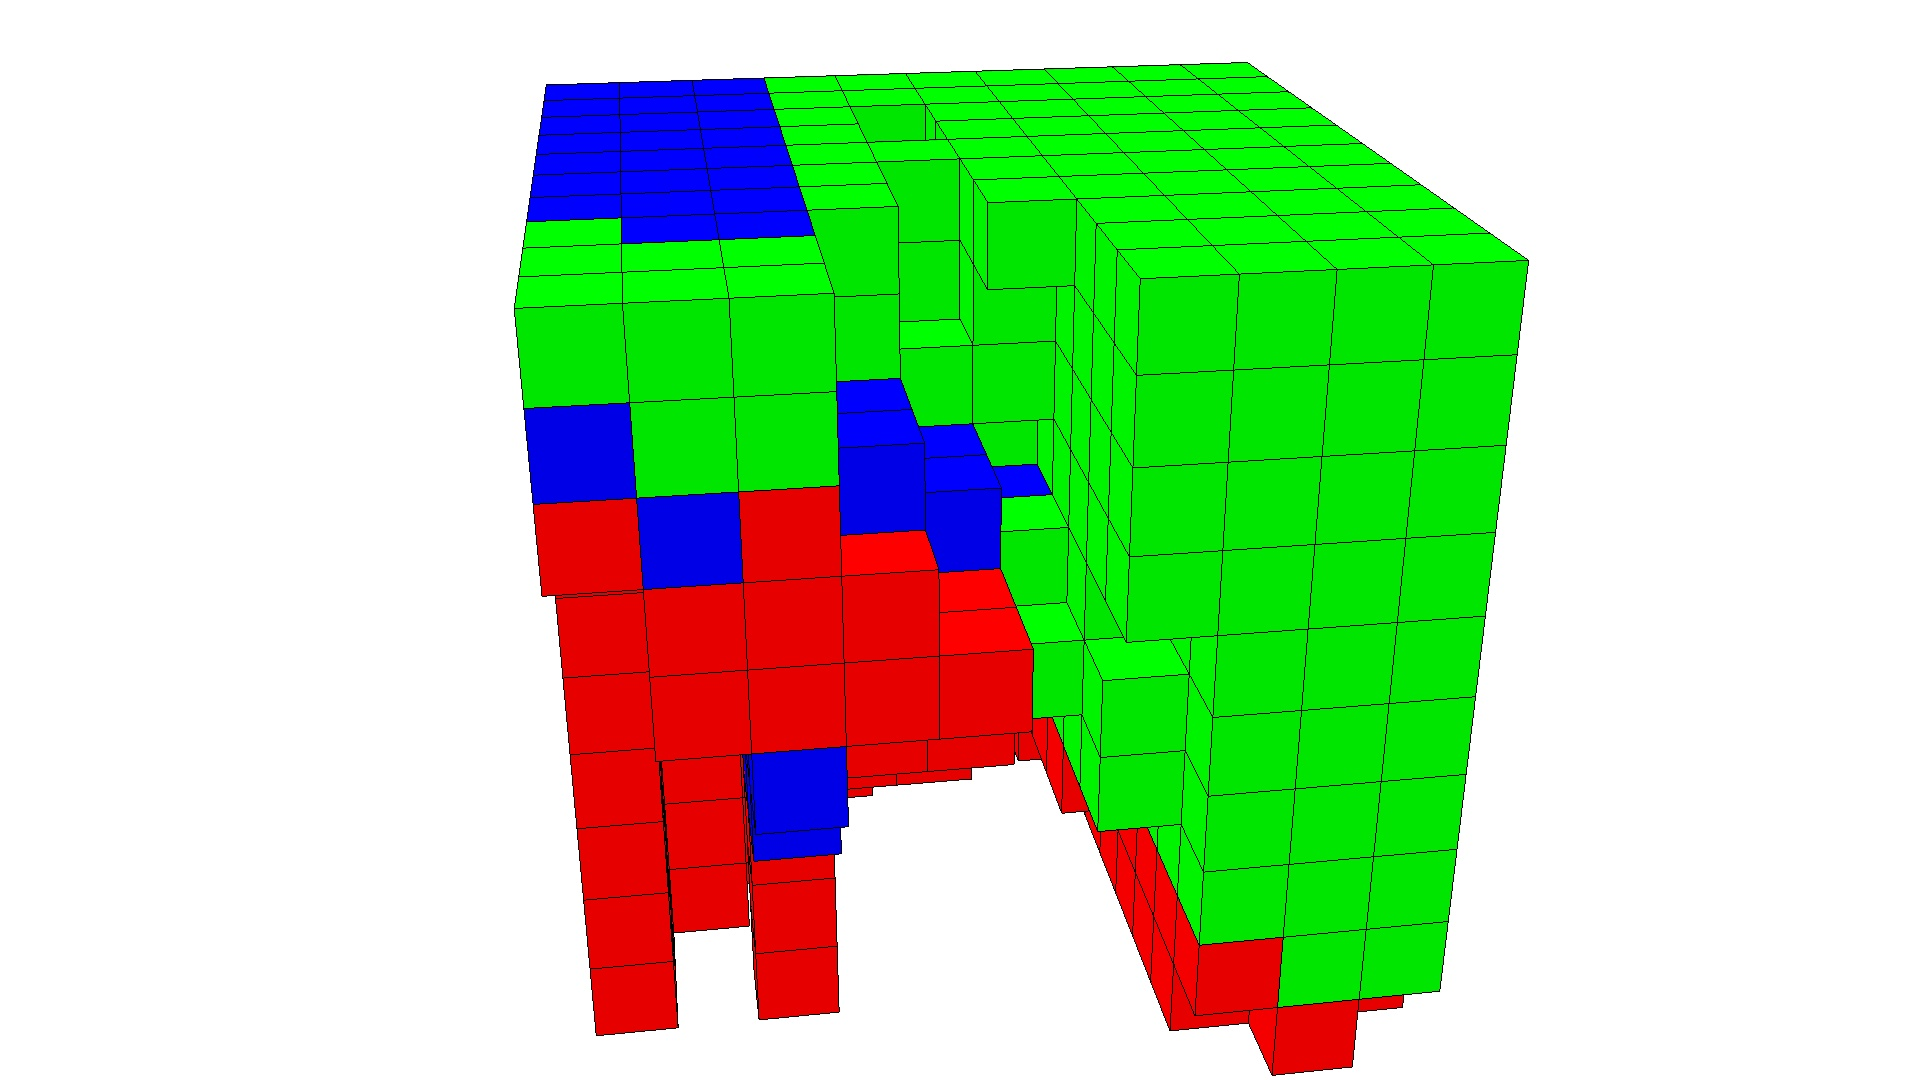
\includegraphics[width=0.19\textwidth]{../Figures/Robots/n_4_g_700.jpg}
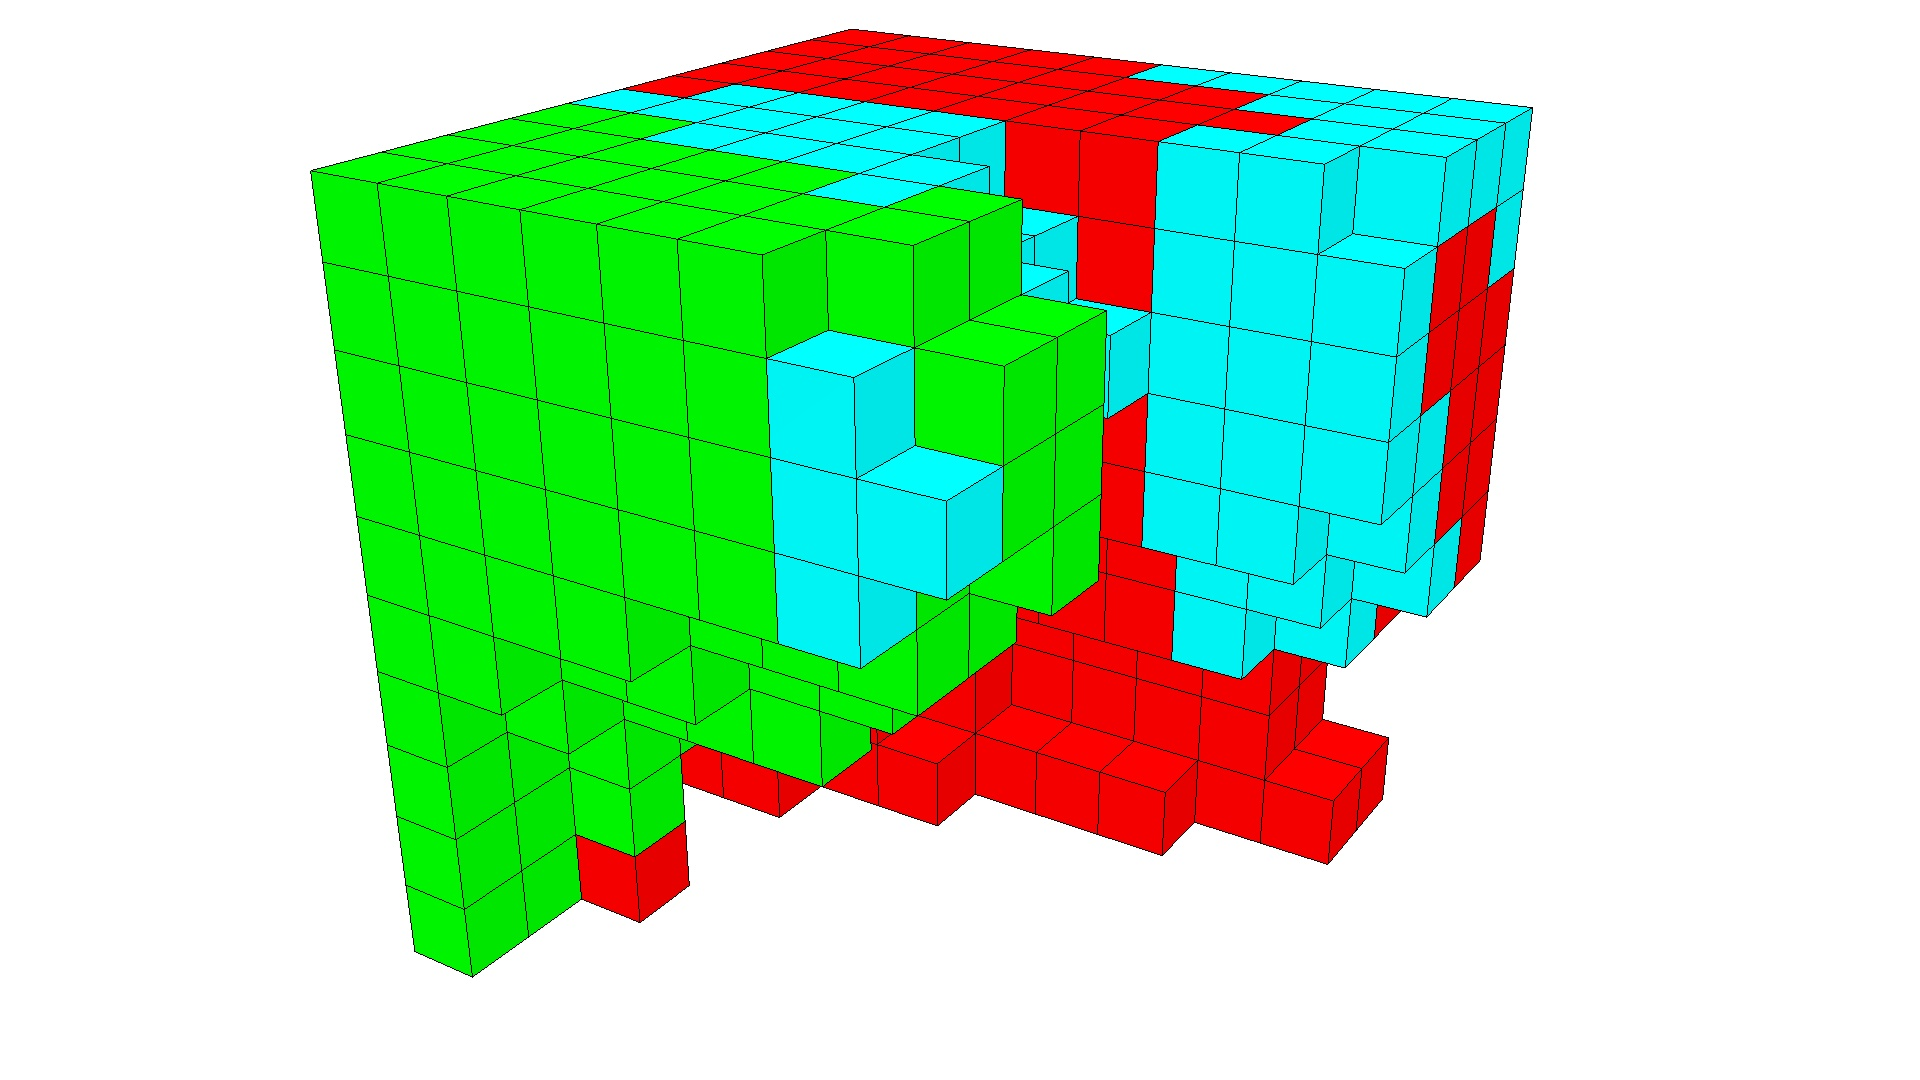
\includegraphics[width=0.19\textwidth]{../Figures/Robots/n_4_g_800.jpg}
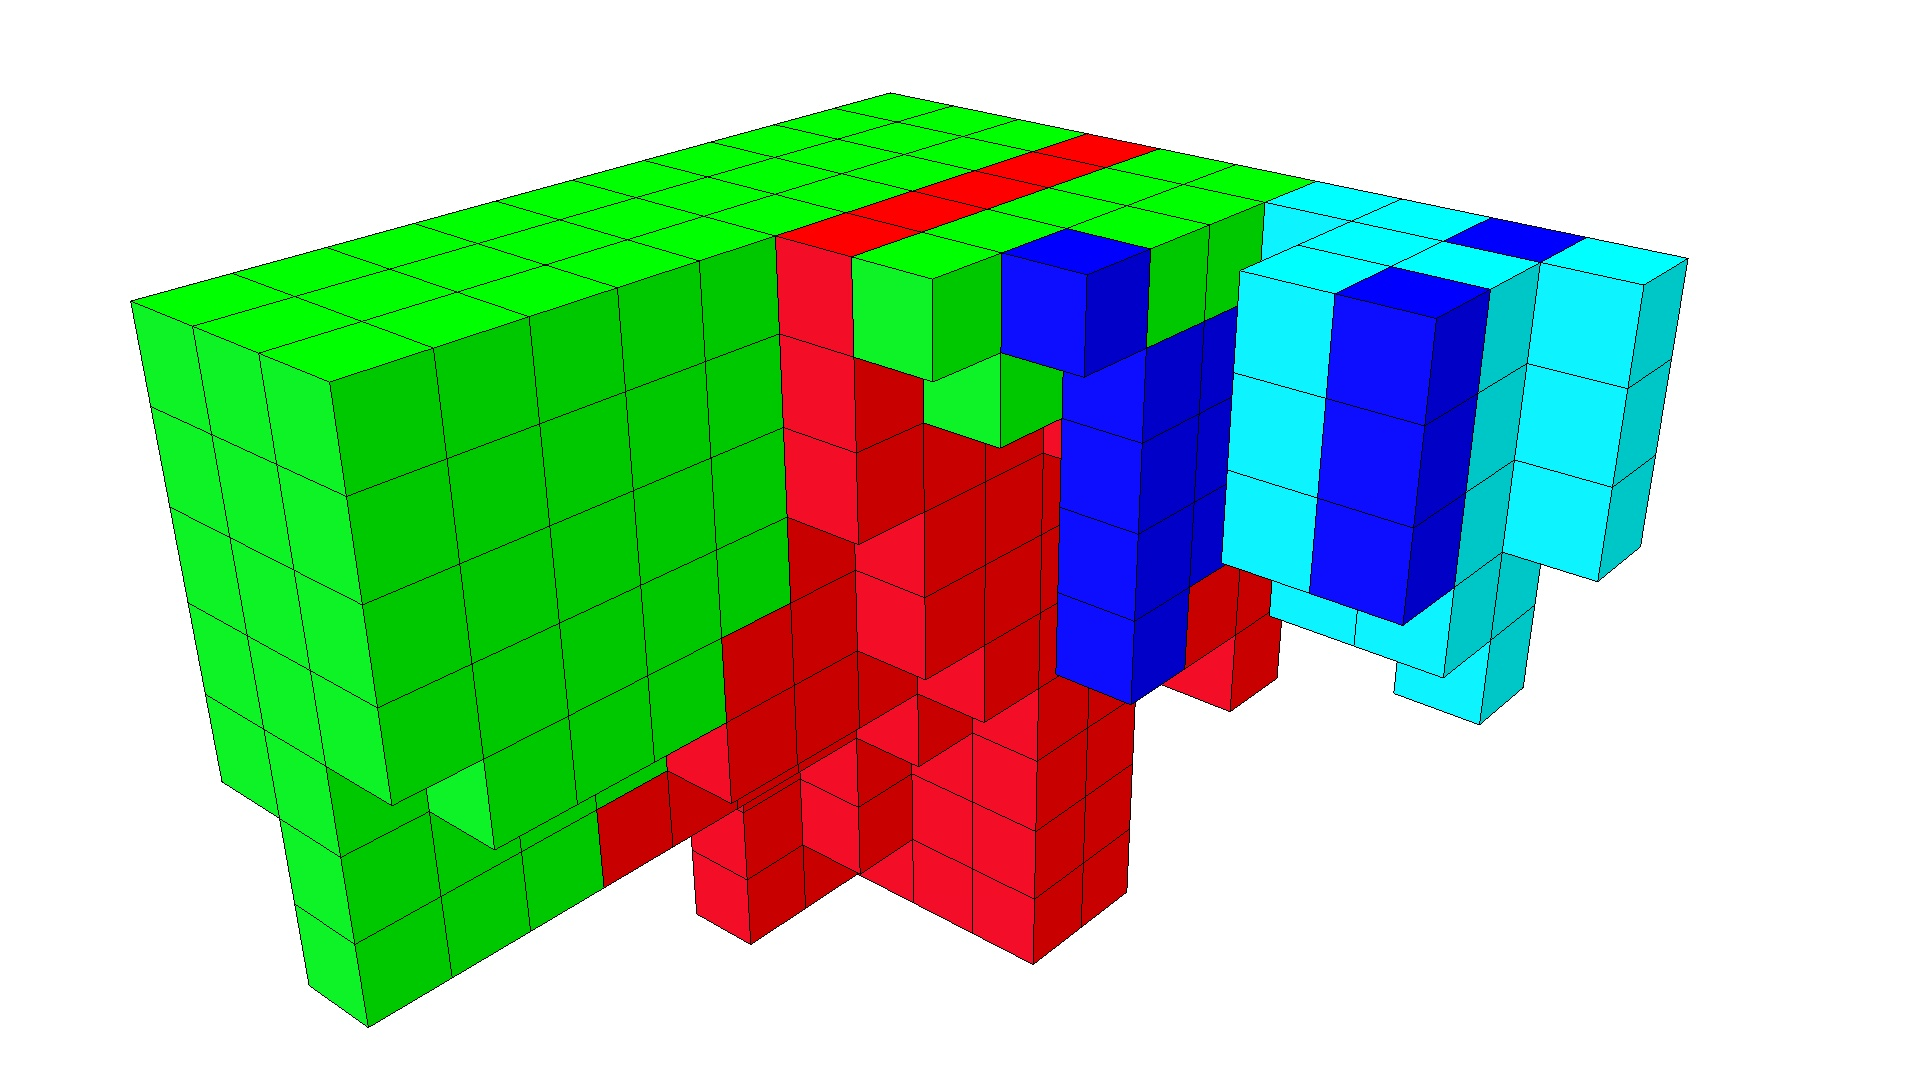
\includegraphics[width=0.19\textwidth]{../Figures/Robots/n_4_g_900.jpg}
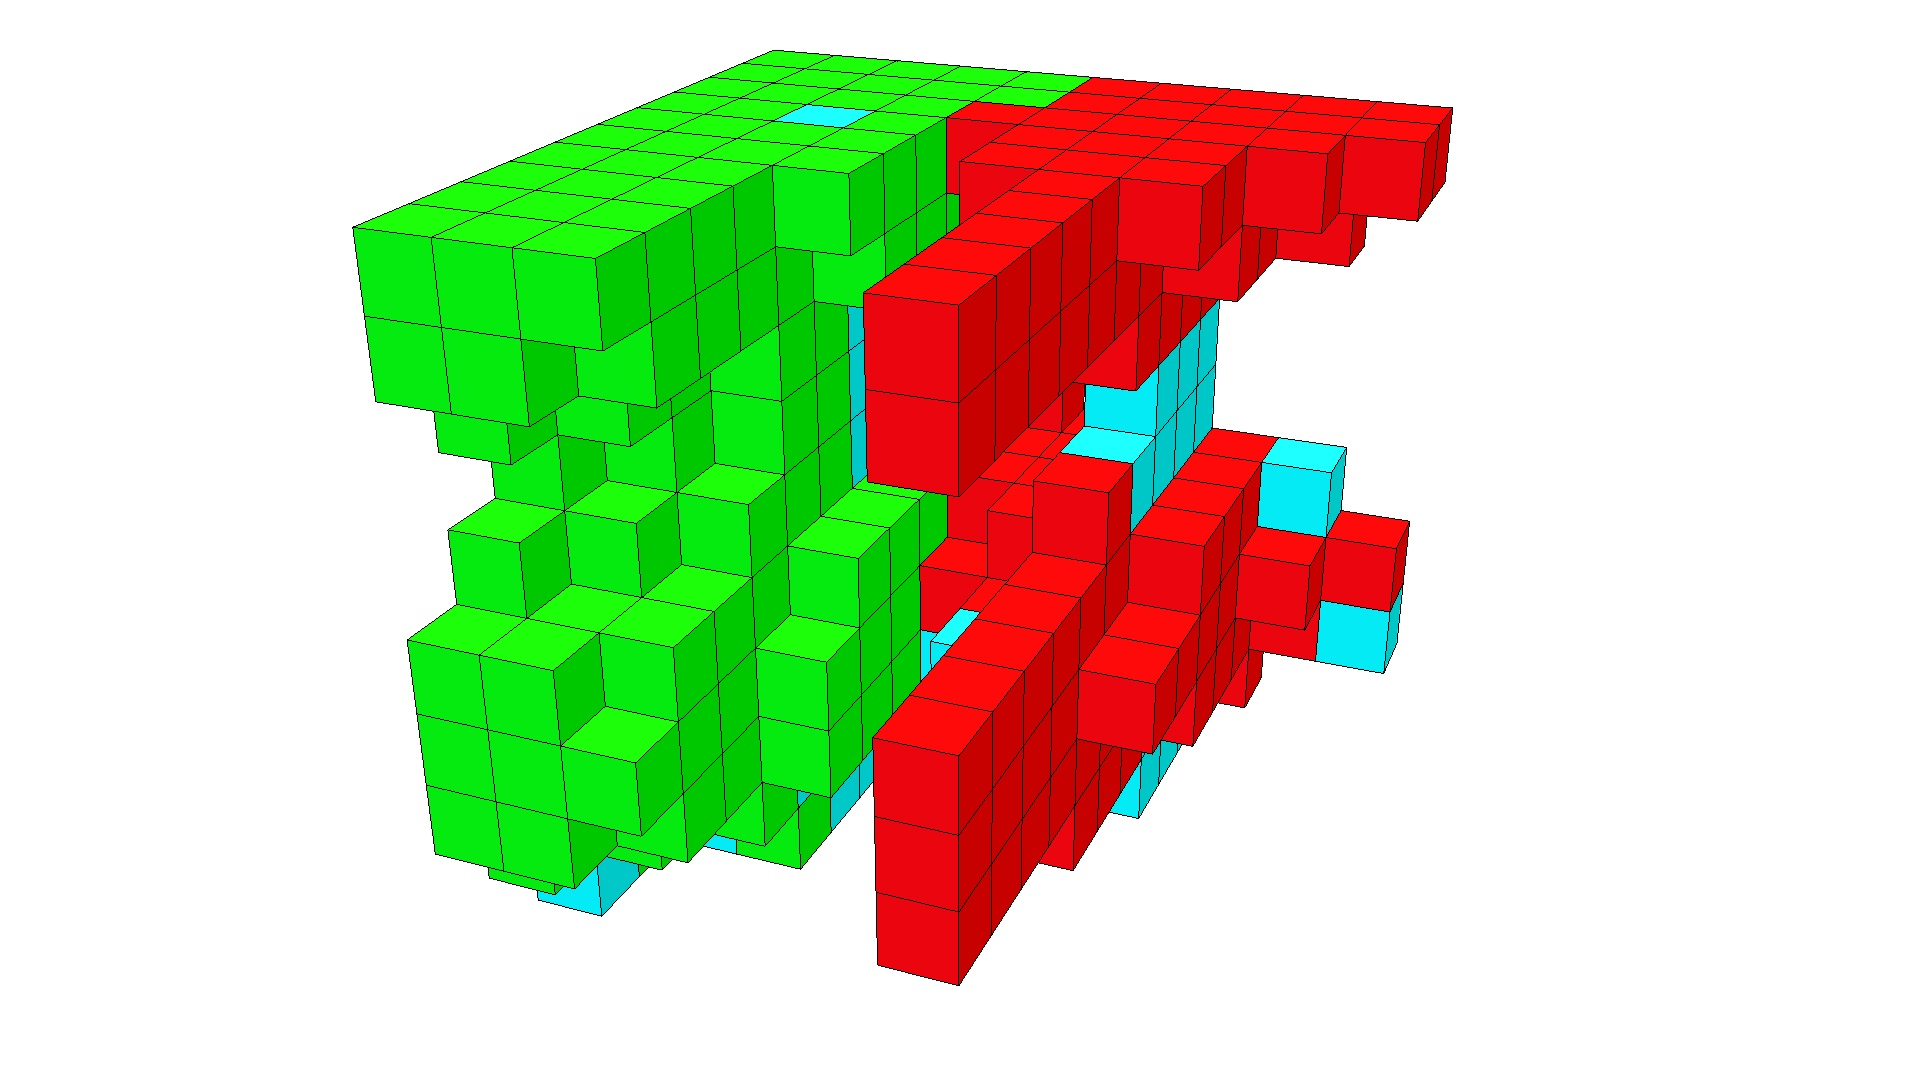
\includegraphics[width=0.19\textwidth]{../Figures/Robots/n_4_g_1000.jpg}
\caption{Novelty search}
\end{subfigure}
\caption{Fitness based search trying to optimize a specific structure while the search for novelty results in a variety of shapes.}
\label{fig:morphologies}
\end{figure}


\subsection{Sparsity in \emph{Novelty}-Search}

Sparsity (eq.~\ref{sparsenessEquation}) is a measure that defines if a newly found behavior is novel enough to enter the set of novel behaviors. Figure~\ref{fig:KnnExperimentSize5} presents the resulted best so far fitness given different values for $k \in \lbrace 1, 2, 5, 10, 20 \rbrace$. In principle $k$ can define how tolerate the algorithm can be with new behaviors. It is not certain that a specific value for $k$ should give the highest performance in fitness and it depends almost completely by the application. The only implication in choosing value for $k$ is that choosing large values should yield in a more detailed exploration in the behavior space, in the contrary using small values final set of behaviors will be denser in the behavior space. In the specific figure and experiment $k=10$ was the setting that led to the best performance.

\subsection{Diversity of Individuals in \emph{Novelty}-Search}

Figure~\ref{fig:morphologies}, shows the champions every hundred generations of a experimental run for novelty search and fitness based search. While the fitness based search is stuck trying to optimize a specific morphology of a soft robots, novelty search is taking a walk in behavior space unveiling new morphologies for the soft-body structures. The same motif appears in every independent run of fitness and novelty search, while novelty search achieves the a variety of morphologies fitness search is sticking to certain shapes, different in every run. It is obvious, that both search methods have their advantages and disadvantages. First, fitness-based search optimizes (optimized distribution of material within the structure) certain shapes during the evolution, at the same time novelty does not optimize them. Novelty search because it is a diversity based method, new shapes are evolved but not optimized. Next section discusses ways of combining both search methods merits.

\begin{figure}[b!]
\centering
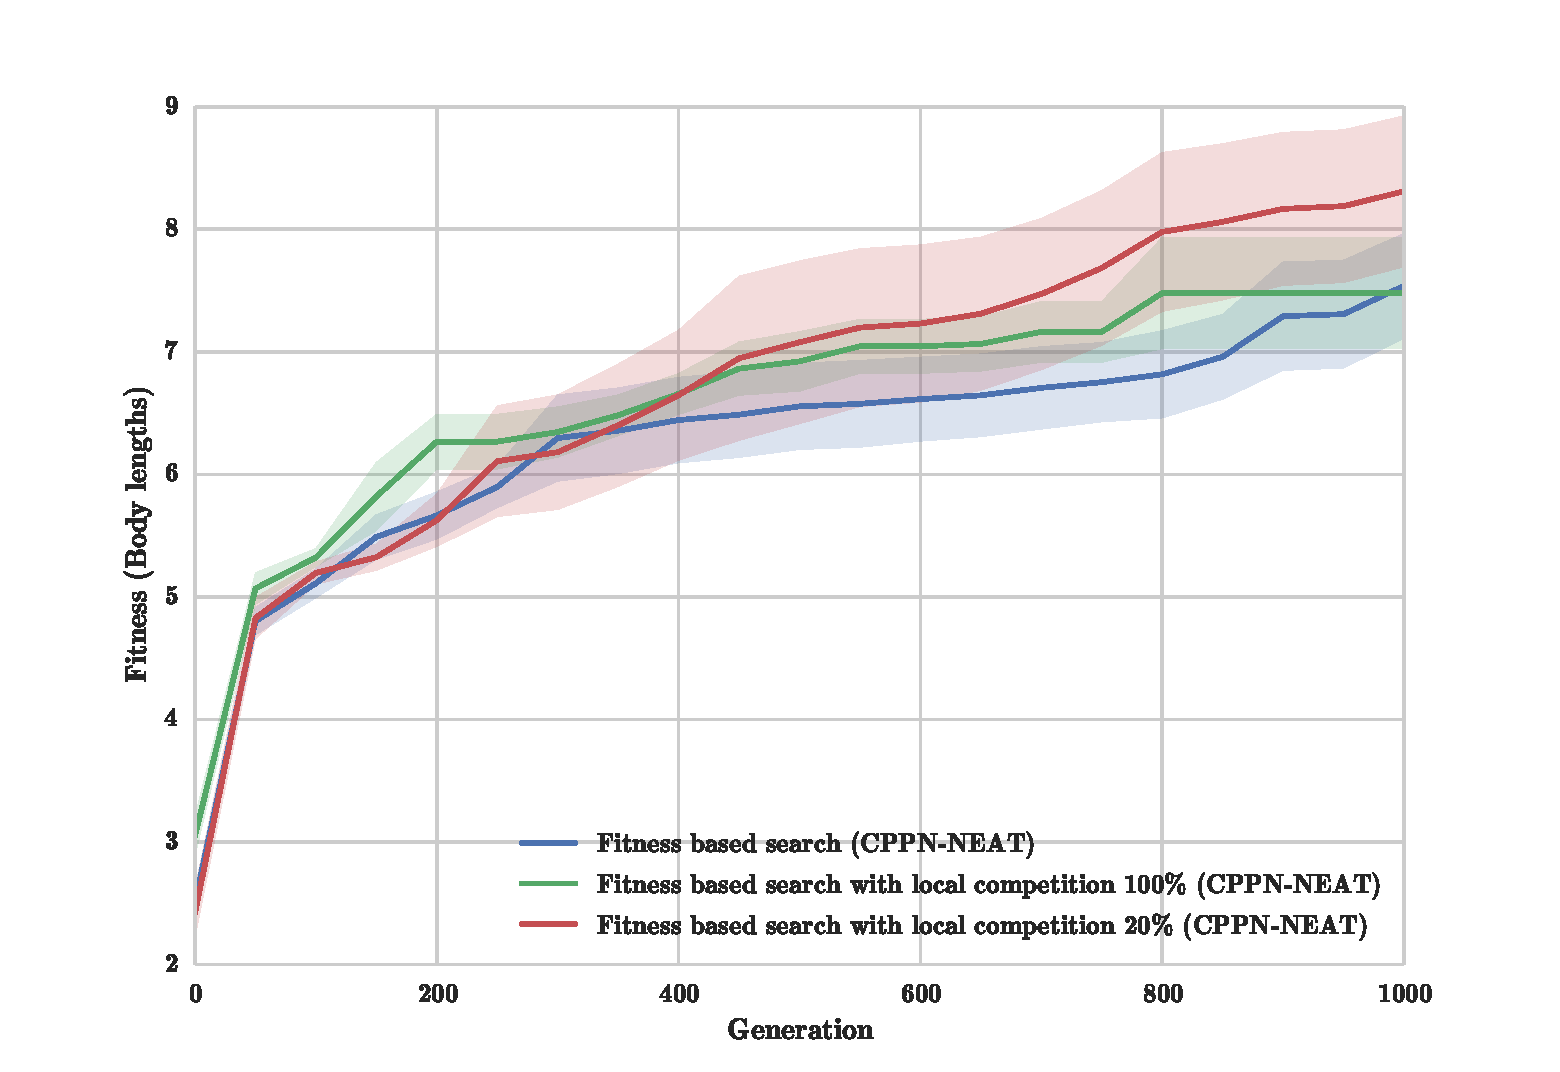
\includegraphics[width=1.0\textwidth]{../Figures/Results/fitComp100_20percent.pdf}
\caption{Best so far fitness averaged over $10$ runs, with no competition, local competition in the complete population of each species for \emph{fitness} search (settings~\ref{Settings3}).}
\label{fig:fitComp100_20percent}
\end{figure}

\section{How Selection Affects the Performance of Both Search Methods}

Discussed extensively in the previous section, selection is a process that picks individuals in order to breed, be mutated or copied into the next generation. It is the part of the evolutionary algorithm that is responsible for producing the new generation, based on the individuals which exist into the current one.


\subsubsection*{\emph{Fitness} Search}

Figure~\ref{fig:fitComp100_20percent}, presents the results for two different selection methods, random selection from the top $20\%$ (\textcolor{MidnightBlue}{Blue}) and competition within individuals from the complete current population (\textcolor{BrickRed}{Red}). As it was expected, competition, as well as, the fact that the whole population has the opportunity to breed, contribute to the diversity of the population. This can be easily seen in this figure, random selection within the top $20\%$ of the population does not allow solution to reproduce meaning that it does not explore weaker individuals, which can later after enough mutations become better than the potential of the rest of the population. The deviation of the first method gives a perfect clue about how narrow is the fitness landscape at the converged area of search when only the best of each generation are allowed to breed.

\subsubsection*{\emph{Novelty} Search}

Since the algorithmic framework is the same for both searches, competition can be applied in novelty search as well. Figure~\ref{fig:NoveltyCompetitionsSize5}, presents the results when competition is held among individual of the whole generation's population among species in respect to different metrics. Competition is held among individual regarding their novelty among the whole population of the evolution and the novelty value they obtain if they are only compared with their species population. In both cases the overall performance of the evolution averaged on $10$ runs is worse than the default setting in novelty search where individuals to breed are selected randomly from the top-$20\%$ of the population of each species. Both selection approaches are performing poorly set side by side with the default selection method. Selecting individuals with high novelty withing the species is crucial for the performance, since these individuals can have low novel value when compared with the global population, leading to steps backwards in the evolution towards highly novel individuals. On the other hand, when individuals are competing using their global novelty measure leads to a slightly better performance, still far from the default setting, meaning that highly novel individuals can actually produce more novel individuals when they are allowed to breed. In other words, competition disturbs  the properties of novelty search, while in fitness based search merits of selecting not only the fittest individuals were shown.


\begin{figure}[t!]
\centering
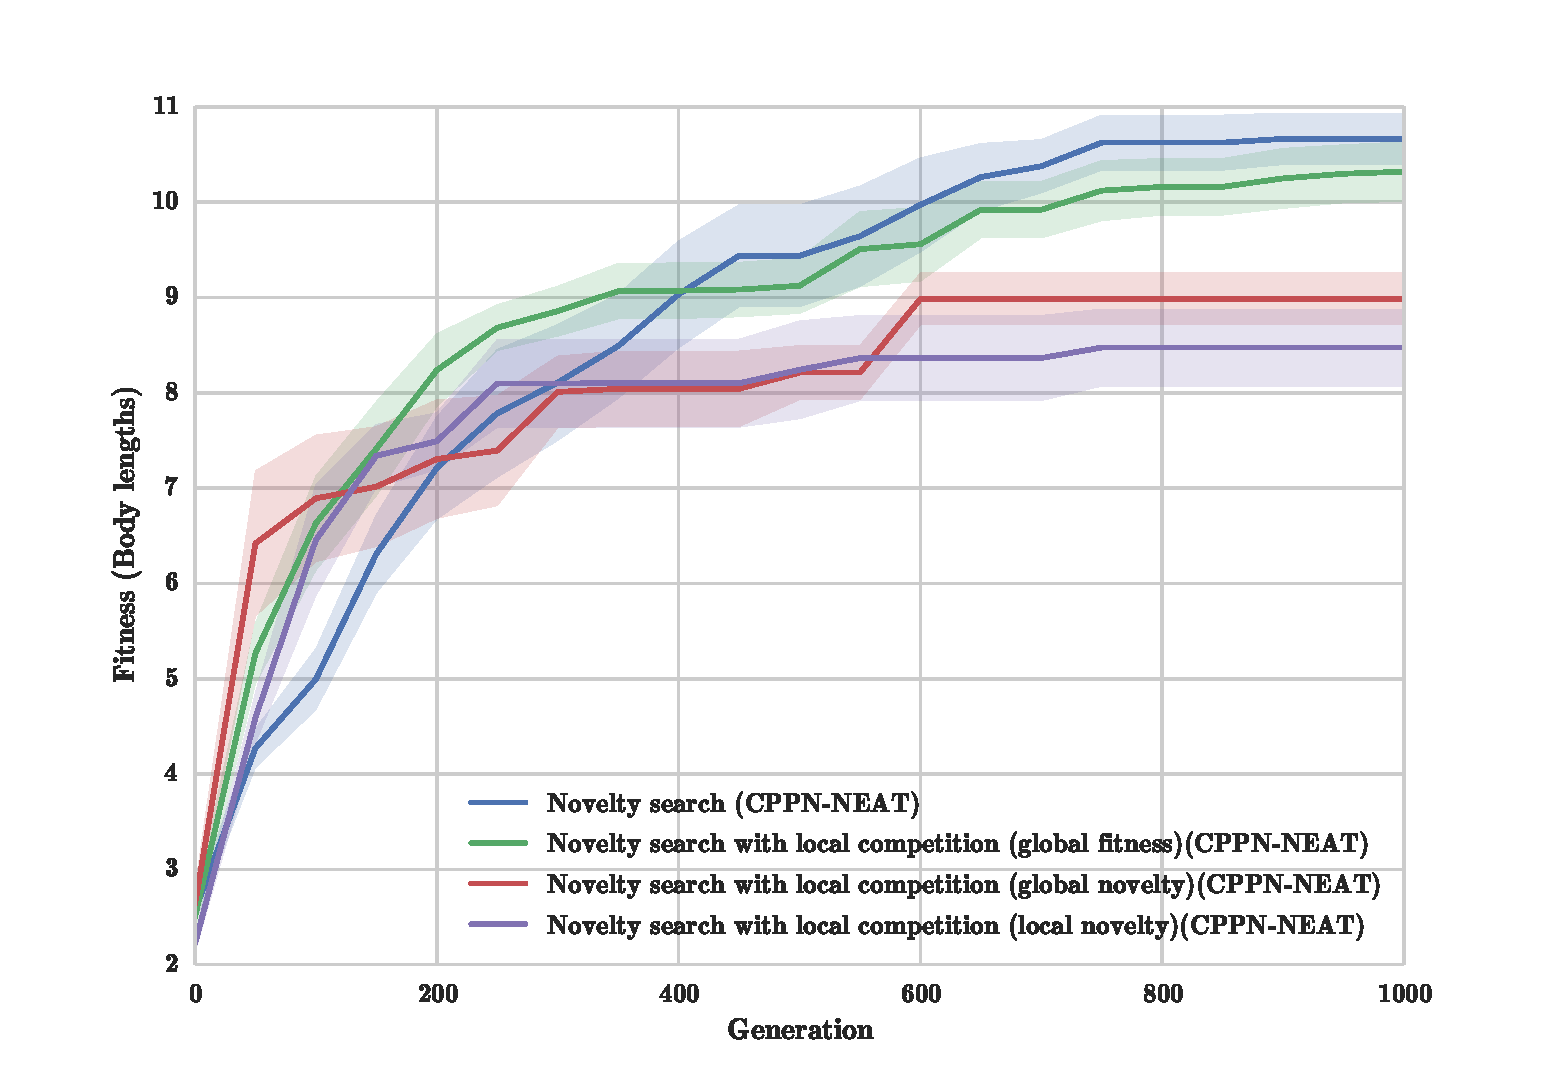
\includegraphics[width=1.0\textwidth]{../Figures/Results/NoveltyCompetitionsSize5.pdf}
\caption{Best so far fitness averaged over $10$ runs, for local competition held among the population of each species for \emph{novelty} search with generative encoding (settings~\ref{Settings1}).}
\label{fig:NoveltyCompetitionsSize5}
\end{figure}



\section{Incorporate \emph{fitness} Information into \emph{Novelty}-Search}

The reason that novelty search is considered such an revolutionary search method is because it finds solutions for deceptive problems, where the fitness landscape is not a straightforward function. What makes it so unique, it is the fact that instead of looking for better solutions in respect to an objective function is looking for different solutions. In each generation of the novelty search there are some solutions that are very good regarding their objective function value, eventually these novel individuals will stop being selected for reproduction since their novelty metric value will be declined as more individuals with similar behaviors will be produced by mutations of the same novel individuals, and they won't be optimized as they could have been. Mutations and other genetic operations can optimize these fit individuals more, but this is something that happens in fitness-based search. These individuals (with high fitness value) can be seen as \emph{stepping~stones}~\cite{lehman2011abandoning} towards more optimized versions of them. Being blind to the objective function, novelty search will eventually stop producing new individuals out of them, which will lead to promising individuals being thrown out of the evolution process. 

Competition is a simple way of combining the two searches together, after each generation is produced competition is held over all the population within each specie, selecting individual, for reproduction, that have high value in the objective function. Figure~\ref{fig:NoveltyCompetitionsSize5}, illustrates the results of using the global fitness as a measure for selection among two generations. The results (\textcolor{ForestGreen}{Green} line), reveal that competition for fitness in a novelty search setting disturbs the balance of the evolution towards novelty, not allowing novelty search to expand the search in a greater extend, since it is not the case that selected fit individuals will lead in novel behaviors. 






\subsection*{Fitness Elitism in Novelty Search}

\begin{figure}[t!]
\centering
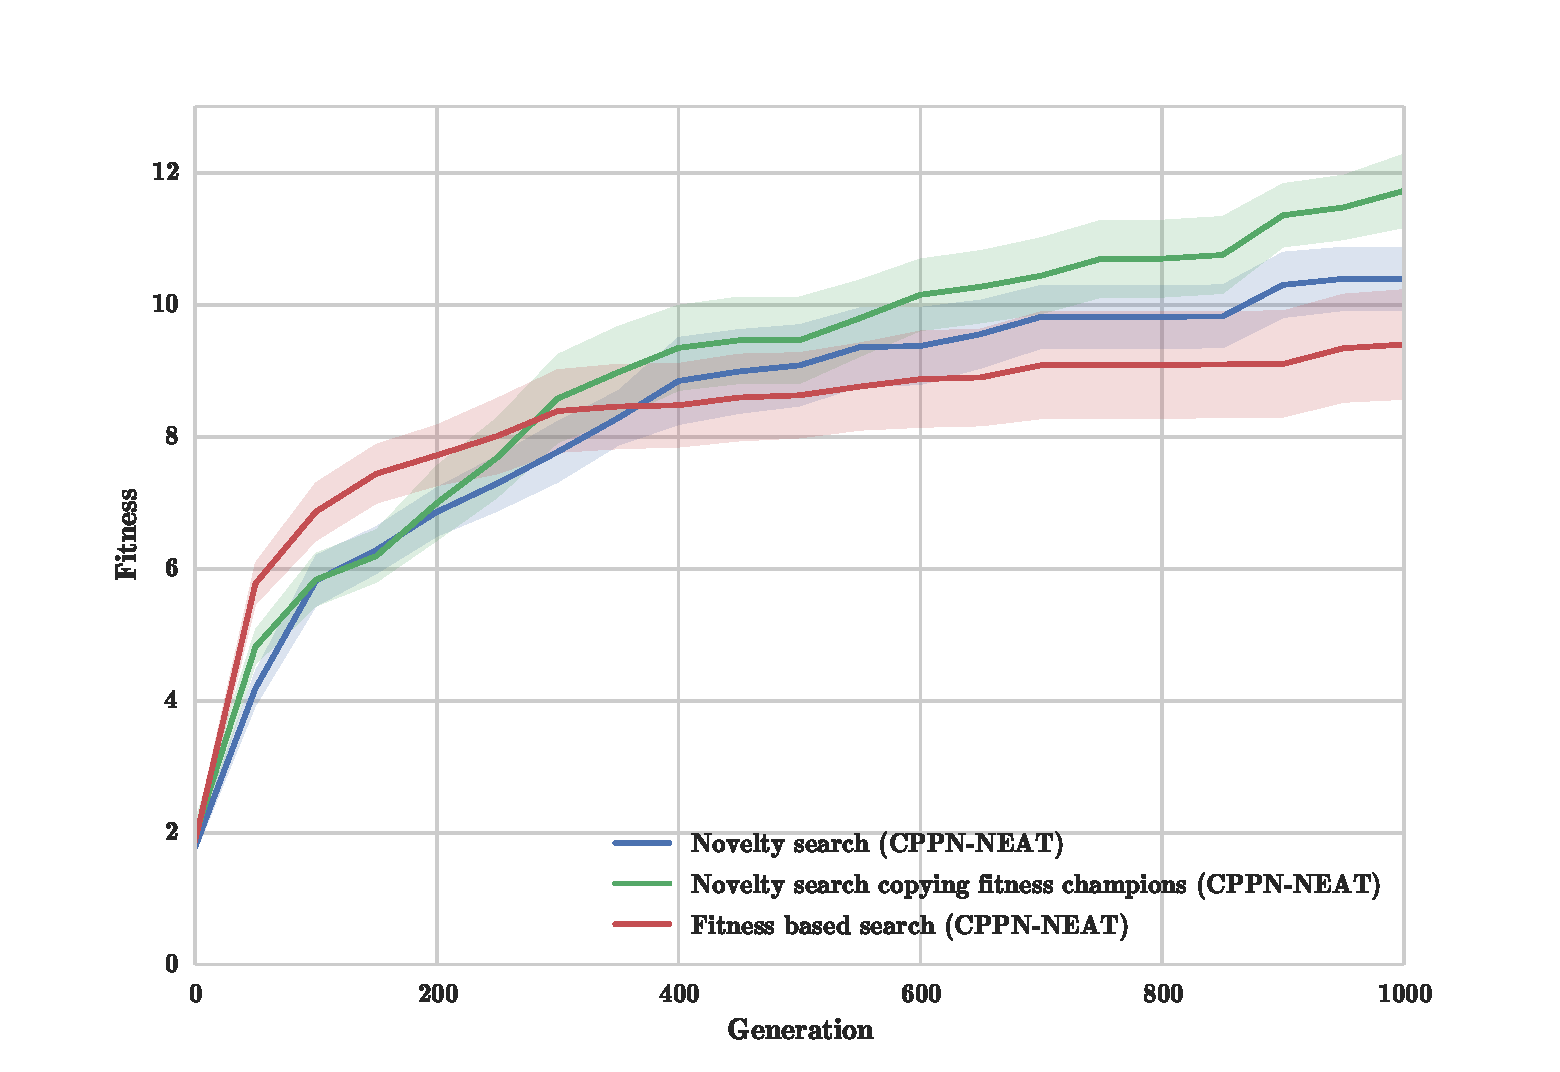
\includegraphics[width=1.0\textwidth]{../Figures/Results/CopyFitChampions10.pdf}
\caption{Best so far fitness averaged over $10$ runs, for \emph{novelty} search with and without copying \emph{fit} champions and \emph{fitness} search (settings~\ref{Settings2}).}
\label{fig:CopyFitChampions10}
\end{figure}

It has been shown, how selecting individuals in respect to their fitness distracts the evolution in novelty search. Hence, a new method is proposed for incorporating fitness information into novelty search without perturbing with its pipeline. Elitism is the process of copying the best individual of each species into the next generation with a probability of mutating it first. In this way best individuals are preserved and can be optimized later, which considered to be a successful way of protecting the best of each species generation so they can contribute with their beneficial genes later in the evolution. Novelty search can include elitism in its selection process, and it does that by copying the most novel organisms of the current population of each species to the next. Since, there is no point of changing this function, elitism can be used also to copy fit individuals within novelty search method. 

The way these two elitism functions can be used depends on the population size, and the problem. Probabilistic methods can also be used combining both elitism functions. In the specific setting, both elitism function copy new individuals to the new generations. In this way the evolution towards novelty does not get disturbed, at the same time, highly fit individuals have the chance to be optimized further as long as they are the fittest within the species population.

Figure~\ref{fig:CopyFitChampions10}, illustrates the gain in performance when fitness elitism is used in novelty search method compared with pure novelty and fitness based search methods.



\section{Evolving Soft-Robots for Outer Space}  

\begin{figure}[t!]
\centering
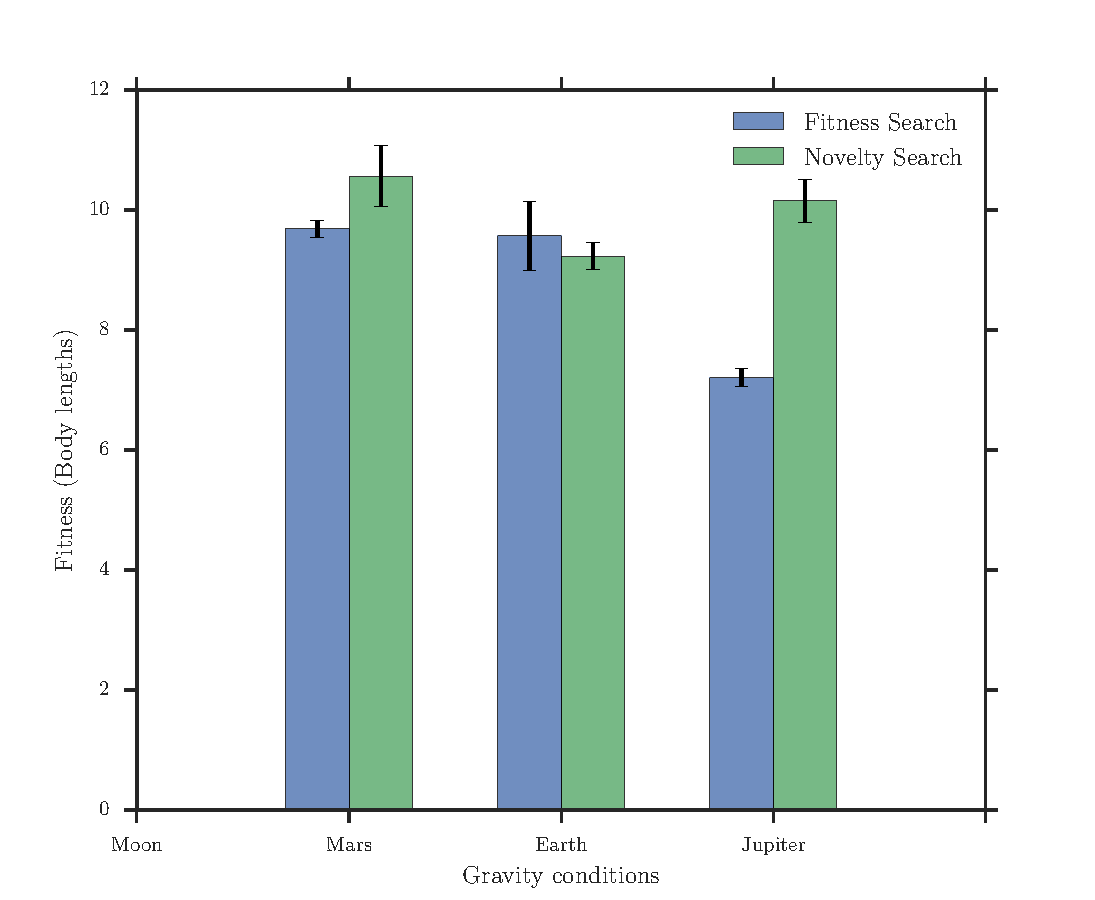
\includegraphics[width=0.8\textwidth]{../Figures/Results/a.pdf}
\caption{Novelty search performs equally good or better than fitness based search in all gravity conditions tested. (settings~\ref{Settings3})} \todo{Experiment not finished yet}
\label{fig:gravityConditions}
\end{figure}

In this section, it is of interest to show how different environmental conditions can affect both the search and the type of locomotion produced by the evolved soft robots. Since, similar conditions of other planets into our solar system are difficult to be reproduced by the simulation environment is used, we only interested to replicate the previous experimental settings with variant gravity acceleration conditions. Fitness based and novelty search are used again within the CPPN-NEAT evolutionary algorithm to evolve the morphology and the locomotion strategies of these voxel structures. For the novelty search two dimensional trajectories of the soft bodies are chosen as the behavior metric to evaluate the novelty of each. 

Figure~\ref{fig:gravityConditions}, illustrates the performance of these two search methods, in four different settings, each method for more than five independent runs, the best fitness achieved by an individual averaged for all runs are shown together with the deviation errors. Default setting used in all previous experiment used for Jupiter's and Earth's gravity accelerations, while the simulation time used for both was $0.4$ seconds. For Moon's and Mars' evolution runs, a higher temperature period was used ($0.050$ seconds), in order effective locomotion to take place, as higher frequencies tend not to be able to  produce any locomotion in lower gravity conditions. Furthermore, for the latter two gravity levels, the simulation time was larger up to $1$ second for each evaluation, as the velocities generated by the soft-robots were significantly lower in such low gravities.

\todo{discuss results}